\documentclass[twoside]{book}

% Packages required by doxygen
\usepackage{fixltx2e}
\usepackage{calc}
\usepackage{doxygen}
\usepackage[export]{adjustbox} % also loads graphicx
\usepackage{graphicx}
\usepackage[utf8]{inputenc}
\usepackage{makeidx}
\usepackage{multicol}
\usepackage{multirow}
\PassOptionsToPackage{warn}{textcomp}
\usepackage{textcomp}
\usepackage[nointegrals]{wasysym}
\usepackage[table]{xcolor}

% Font selection
\usepackage[T1]{fontenc}
\usepackage[scaled=.90]{helvet}
\usepackage{courier}
\usepackage{amssymb}
\usepackage{sectsty}
\renewcommand{\familydefault}{\sfdefault}
\allsectionsfont{%
  \fontseries{bc}\selectfont%
  \color{darkgray}%
}
\renewcommand{\DoxyLabelFont}{%
  \fontseries{bc}\selectfont%
  \color{darkgray}%
}
\newcommand{\+}{\discretionary{\mbox{\scriptsize$\hookleftarrow$}}{}{}}

% Page & text layout
\usepackage{geometry}
\geometry{%
  a4paper,%
  top=2.5cm,%
  bottom=2.5cm,%
  left=2.5cm,%
  right=2.5cm%
}
\tolerance=750
\hfuzz=15pt
\hbadness=750
\setlength{\emergencystretch}{15pt}
\setlength{\parindent}{0cm}
\setlength{\parskip}{3ex plus 2ex minus 2ex}
\makeatletter
\renewcommand{\paragraph}{%
  \@startsection{paragraph}{4}{0ex}{-1.0ex}{1.0ex}{%
    \normalfont\normalsize\bfseries\SS@parafont%
  }%
}
\renewcommand{\subparagraph}{%
  \@startsection{subparagraph}{5}{0ex}{-1.0ex}{1.0ex}{%
    \normalfont\normalsize\bfseries\SS@subparafont%
  }%
}
\makeatother

% Headers & footers
\usepackage{fancyhdr}
\pagestyle{fancyplain}
\fancyhead[LE]{\fancyplain{}{\bfseries\thepage}}
\fancyhead[CE]{\fancyplain{}{}}
\fancyhead[RE]{\fancyplain{}{\bfseries\leftmark}}
\fancyhead[LO]{\fancyplain{}{\bfseries\rightmark}}
\fancyhead[CO]{\fancyplain{}{}}
\fancyhead[RO]{\fancyplain{}{\bfseries\thepage}}
\fancyfoot[LE]{\fancyplain{}{}}
\fancyfoot[CE]{\fancyplain{}{}}
\fancyfoot[RE]{\fancyplain{}{\bfseries\scriptsize Generated by Doxygen }}
\fancyfoot[LO]{\fancyplain{}{\bfseries\scriptsize Generated by Doxygen }}
\fancyfoot[CO]{\fancyplain{}{}}
\fancyfoot[RO]{\fancyplain{}{}}
\renewcommand{\footrulewidth}{0.4pt}
\renewcommand{\chaptermark}[1]{%
  \markboth{#1}{}%
}
\renewcommand{\sectionmark}[1]{%
  \markright{\thesection\ #1}%
}

% Indices & bibliography
\usepackage{natbib}
\usepackage[titles]{tocloft}
\setcounter{tocdepth}{3}
\setcounter{secnumdepth}{5}
\makeindex

% Hyperlinks (required, but should be loaded last)
\usepackage{ifpdf}
\ifpdf
  \usepackage[pdftex,pagebackref=true]{hyperref}
\else
  \usepackage[ps2pdf,pagebackref=true]{hyperref}
\fi
\hypersetup{%
  colorlinks=true,%
  linkcolor=blue,%
  citecolor=blue,%
  unicode%
}

% Custom commands
\newcommand{\clearemptydoublepage}{%
  \newpage{\pagestyle{empty}\cleardoublepage}%
}

\usepackage{caption}
\captionsetup{labelsep=space,justification=centering,font={bf},singlelinecheck=off,skip=4pt,position=top}

%===== C O N T E N T S =====

\begin{document}

% Titlepage & ToC
\hypersetup{pageanchor=false,
             bookmarksnumbered=true,
             pdfencoding=unicode
            }
\pagenumbering{alph}
\begin{titlepage}
\vspace*{7cm}
\begin{center}%
{\Large Projekt\+: Autonomes Fahren }\\
\vspace*{1cm}
{\large Generated by Doxygen 1.8.14}\\
\end{center}
\end{titlepage}
\clearemptydoublepage
\pagenumbering{roman}
\tableofcontents
\clearemptydoublepage
\pagenumbering{arabic}
\hypersetup{pageanchor=true}

%--- Begin generated contents ---
\chapter{Hierarchical Index}
\section{Class Hierarchy}
This inheritance list is sorted roughly, but not completely, alphabetically\+:\begin{DoxyCompactList}
\item \contentsline{section}{Caretaker}{\pageref{class_caretaker}}{}
\item \contentsline{section}{Connection}{\pageref{struct_connection}}{}
\item \contentsline{section}{Map}{\pageref{class_map}}{}
\item \contentsline{section}{Memento}{\pageref{class_memento}}{}
\item \contentsline{section}{neural\+Net}{\pageref{classneural_net}}{}
\item \contentsline{section}{Neuron}{\pageref{class_neuron}}{}
\item \contentsline{section}{Point}{\pageref{class_point}}{}
\item Q\+Graphics\+Item\begin{DoxyCompactList}
\item \contentsline{section}{Obstacle}{\pageref{class_obstacle}}{}
\begin{DoxyCompactList}
\item \contentsline{section}{Dynamic\+Obstacle}{\pageref{class_dynamic_obstacle}}{}
\end{DoxyCompactList}
\item \contentsline{section}{Sensor}{\pageref{class_sensor}}{}
\item \contentsline{section}{Smart\+Vehicle}{\pageref{class_smart_vehicle}}{}
\item \contentsline{section}{Tile}{\pageref{class_tile}}{}
\begin{DoxyCompactList}
\item \contentsline{section}{Endingtile}{\pageref{class_endingtile}}{}
\item \contentsline{section}{Intersection}{\pageref{class_intersection}}{}
\item \contentsline{section}{Startingtile}{\pageref{class_startingtile}}{}
\item \contentsline{section}{straight}{\pageref{classstraight}}{}
\item \contentsline{section}{Tintersection}{\pageref{class_tintersection}}{}
\item \contentsline{section}{turn}{\pageref{classturn}}{}
\end{DoxyCompactList}
\end{DoxyCompactList}
\item Q\+Main\+Window\begin{DoxyCompactList}
\item \contentsline{section}{Editor}{\pageref{class_editor}}{}
\item \contentsline{section}{Simulator}{\pageref{class_simulator}}{}
\item \contentsline{section}{Simulator\+Window}{\pageref{class_simulator_window}}{}
\end{DoxyCompactList}
\item Q\+Object\begin{DoxyCompactList}
\item \contentsline{section}{Simulator\+C\+M\+DL}{\pageref{class_simulator_c_m_d_l}}{}
\end{DoxyCompactList}
\end{DoxyCompactList}

\chapter{Class Index}
\section{Class List}
Here are the classes, structs, unions and interfaces with brief descriptions\+:\begin{DoxyCompactList}
\item\contentsline{section}{\mbox{\hyperlink{class_caretaker}{Caretaker}} }{\pageref{class_caretaker}}{}
\item\contentsline{section}{\mbox{\hyperlink{struct_connection}{Connection}} }{\pageref{struct_connection}}{}
\item\contentsline{section}{\mbox{\hyperlink{class_dynamic_obstacle}{Dynamic\+Obstacle}} }{\pageref{class_dynamic_obstacle}}{}
\item\contentsline{section}{\mbox{\hyperlink{class_editor}{Editor}} }{\pageref{class_editor}}{}
\item\contentsline{section}{\mbox{\hyperlink{class_endingtile}{Endingtile}} }{\pageref{class_endingtile}}{}
\item\contentsline{section}{\mbox{\hyperlink{class_intersection}{Intersection}} }{\pageref{class_intersection}}{}
\item\contentsline{section}{\mbox{\hyperlink{class_map}{Map}} }{\pageref{class_map}}{}
\item\contentsline{section}{\mbox{\hyperlink{class_memento}{Memento}} }{\pageref{class_memento}}{}
\item\contentsline{section}{\mbox{\hyperlink{classneural_net}{neural\+Net}} }{\pageref{classneural_net}}{}
\item\contentsline{section}{\mbox{\hyperlink{class_neuron}{Neuron}} }{\pageref{class_neuron}}{}
\item\contentsline{section}{\mbox{\hyperlink{class_obstacle}{Obstacle}} }{\pageref{class_obstacle}}{}
\item\contentsline{section}{\mbox{\hyperlink{class_point}{Point}} }{\pageref{class_point}}{}
\item\contentsline{section}{\mbox{\hyperlink{class_sensor}{Sensor}} }{\pageref{class_sensor}}{}
\item\contentsline{section}{\mbox{\hyperlink{class_simulator}{Simulator}} }{\pageref{class_simulator}}{}
\item\contentsline{section}{\mbox{\hyperlink{class_simulator_c_m_d_l}{Simulator\+C\+M\+DL}} }{\pageref{class_simulator_c_m_d_l}}{}
\item\contentsline{section}{\mbox{\hyperlink{class_simulator_window}{Simulator\+Window}} }{\pageref{class_simulator_window}}{}
\item\contentsline{section}{\mbox{\hyperlink{class_smart_vehicle}{Smart\+Vehicle}} }{\pageref{class_smart_vehicle}}{}
\item\contentsline{section}{\mbox{\hyperlink{class_startingtile}{Startingtile}} }{\pageref{class_startingtile}}{}
\item\contentsline{section}{\mbox{\hyperlink{classstraight}{straight}} }{\pageref{classstraight}}{}
\item\contentsline{section}{\mbox{\hyperlink{class_tile}{Tile}} }{\pageref{class_tile}}{}
\item\contentsline{section}{\mbox{\hyperlink{class_tintersection}{Tintersection}} }{\pageref{class_tintersection}}{}
\item\contentsline{section}{\mbox{\hyperlink{classturn}{turn}} }{\pageref{classturn}}{}
\end{DoxyCompactList}

\chapter{Class Documentation}
\hypertarget{class_caretaker}{}\section{Caretaker Class Reference}
\label{class_caretaker}\index{Caretaker@{Caretaker}}
\subsection*{Public Member Functions}
\begin{DoxyCompactItemize}
\item 
\mbox{\Hypertarget{class_caretaker_add41f564551d753809fbe168cd38008a}\label{class_caretaker_add41f564551d753809fbe168cd38008a}} 
\mbox{\hyperlink{class_memento}{Memento}} $\ast$ {\bfseries get\+Memento} ()
\item 
\mbox{\Hypertarget{class_caretaker_ad4cc3a4e331e21e0333b8af8e1571782}\label{class_caretaker_ad4cc3a4e331e21e0333b8af8e1571782}} 
void {\bfseries set\+Memento} (\mbox{\hyperlink{class_memento}{Memento}} $\ast$m)
\item 
\mbox{\Hypertarget{class_caretaker_aafcf9acc1689fc7728b2f8115a413ecc}\label{class_caretaker_aafcf9acc1689fc7728b2f8115a413ecc}} 
void {\bfseries delete\+Last} ()
\item 
\mbox{\Hypertarget{class_caretaker_a756d877f9f4484243549f27b21dfd586}\label{class_caretaker_a756d877f9f4484243549f27b21dfd586}} 
int {\bfseries get\+Mem\+Size} ()
\end{DoxyCompactItemize}


The documentation for this class was generated from the following files\+:\begin{DoxyCompactItemize}
\item 
D\+:/swt1718-\/editor/bin/source/caretaker.\+h\item 
D\+:/swt1718-\/editor/bin/source/caretaker.\+cpp\end{DoxyCompactItemize}

\hypertarget{struct_connection}{}\section{Connection Struct Reference}
\label{struct_connection}\index{Connection@{Connection}}
\subsection*{Public Attributes}
\begin{DoxyCompactItemize}
\item 
\mbox{\Hypertarget{struct_connection_ab945ccb1a81e582abd5938f67af69390}\label{struct_connection_ab945ccb1a81e582abd5938f67af69390}} 
double {\bfseries weight}
\item 
\mbox{\Hypertarget{struct_connection_a9f74bf311cc02e9f2e17ca28baf74fab}\label{struct_connection_a9f74bf311cc02e9f2e17ca28baf74fab}} 
double {\bfseries delta\+Weight}
\end{DoxyCompactItemize}


The documentation for this struct was generated from the following file\+:\begin{DoxyCompactItemize}
\item 
D\+:/swt1718-\/editor/bin/source/neuron.\+h\end{DoxyCompactItemize}

\hypertarget{class_dynamic_obstacle}{}\section{Dynamic\+Obstacle Class Reference}
\label{class_dynamic_obstacle}\index{Dynamic\+Obstacle@{Dynamic\+Obstacle}}
Inheritance diagram for Dynamic\+Obstacle\+:\begin{figure}[H]
\begin{center}
\leavevmode
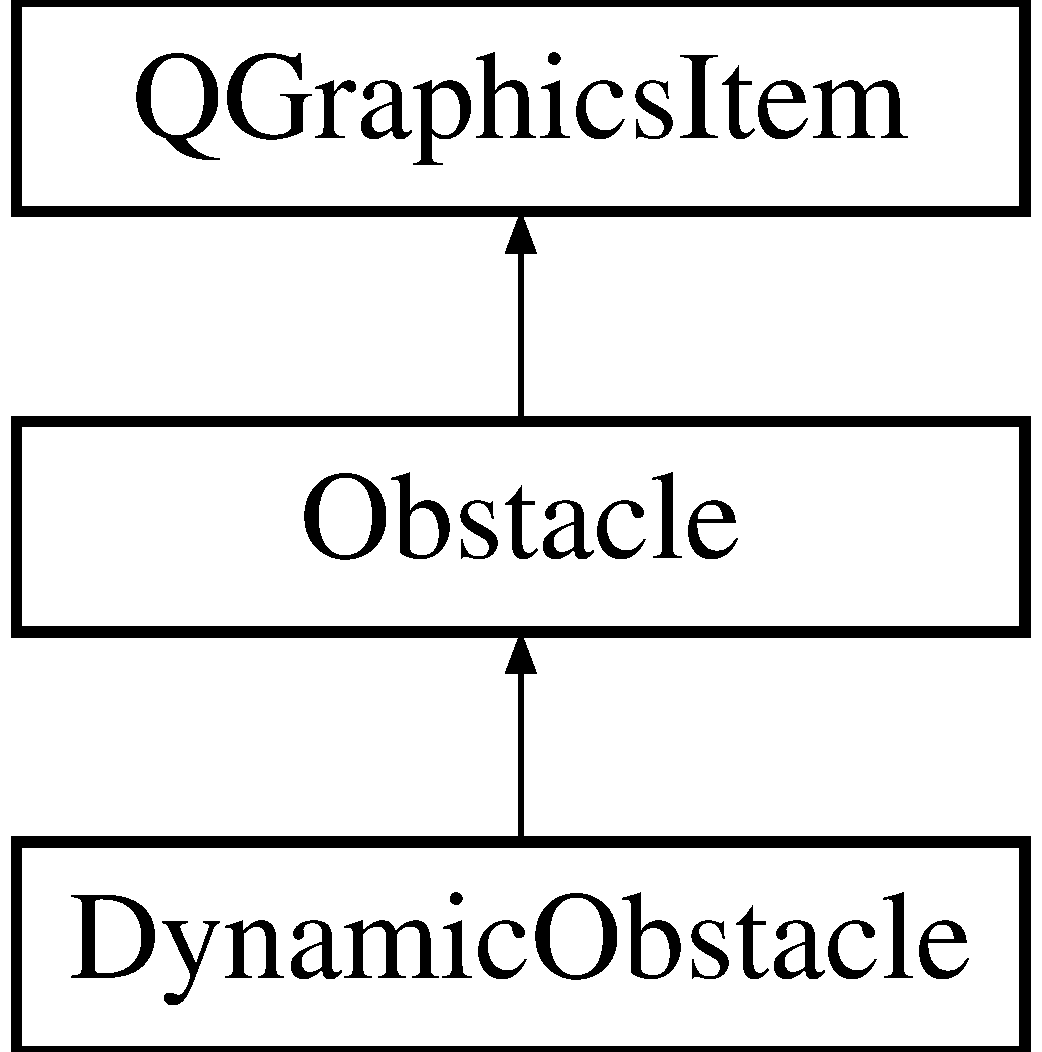
\includegraphics[height=3.000000cm]{class_dynamic_obstacle}
\end{center}
\end{figure}
\subsection*{Public Member Functions}
\begin{DoxyCompactItemize}
\item 
\mbox{\Hypertarget{class_dynamic_obstacle_a5a4ea17aa7b7fe99f9a627aa762b1f5b}\label{class_dynamic_obstacle_a5a4ea17aa7b7fe99f9a627aa762b1f5b}} 
void {\bfseries accelerate} (double acc=0.\+1)
\item 
\mbox{\Hypertarget{class_dynamic_obstacle_a158690143090a4b8001f411db9b6c1e0}\label{class_dynamic_obstacle_a158690143090a4b8001f411db9b6c1e0}} 
void {\bfseries brake} (double br=0.\+1)
\item 
\mbox{\Hypertarget{class_dynamic_obstacle_ab7968cfdaab0d81fcb75db774de1adb2}\label{class_dynamic_obstacle_ab7968cfdaab0d81fcb75db774de1adb2}} 
double {\bfseries get\+Speed} ()
\item 
\mbox{\Hypertarget{class_dynamic_obstacle_ab4ca72e5c4f18fdac9dd43cf26fe1d35}\label{class_dynamic_obstacle_ab4ca72e5c4f18fdac9dd43cf26fe1d35}} 
void {\bfseries set\+Speed} (double s)
\item 
\mbox{\Hypertarget{class_dynamic_obstacle_a3f4321cfcfd9c480bf779042228b8de1}\label{class_dynamic_obstacle_a3f4321cfcfd9c480bf779042228b8de1}} 
int {\bfseries get\+Direction} ()
\item 
\mbox{\Hypertarget{class_dynamic_obstacle_ab1bf58416de0faf82f18c0d2c42ba000}\label{class_dynamic_obstacle_ab1bf58416de0faf82f18c0d2c42ba000}} 
void {\bfseries set\+Direction} (int d)
\item 
\mbox{\Hypertarget{class_dynamic_obstacle_a1ff562d7a0c22eb41cdd86f71d964a4e}\label{class_dynamic_obstacle_a1ff562d7a0c22eb41cdd86f71d964a4e}} 
double {\bfseries calculate\+Rotation} ()
\item 
Q\+RectF \mbox{\hyperlink{class_dynamic_obstacle_ac1b0b15d722a45decc8b77fcde22efd0}{bounding\+Rect}} () const
\item 
void \mbox{\hyperlink{class_dynamic_obstacle_a30c0753280f05f69a9da89bc9d9ce3f6}{paint}} (Q\+Painter $\ast$painter, const Q\+Style\+Option\+Graphics\+Item $\ast$option, Q\+Widget $\ast$widget)
\item 
Q\+String \mbox{\hyperlink{class_dynamic_obstacle_ac52c38ef60b99a7a29f89b6eb23df460}{get\+Type}} ()
\item 
\mbox{\Hypertarget{class_dynamic_obstacle_a6dae975b1b2abe86f62ab1df11d19293}\label{class_dynamic_obstacle_a6dae975b1b2abe86f62ab1df11d19293}} 
void {\bfseries set\+Starting\+Point} (Q\+PointF s)
\item 
\mbox{\Hypertarget{class_dynamic_obstacle_a17645d997a7c2a7deaf5fe4726421097}\label{class_dynamic_obstacle_a17645d997a7c2a7deaf5fe4726421097}} 
void {\bfseries set\+Ending\+Point} (Q\+PointF e)
\item 
\mbox{\Hypertarget{class_dynamic_obstacle_ad2eb80be1ef5df9f1ff70d200751c818}\label{class_dynamic_obstacle_ad2eb80be1ef5df9f1ff70d200751c818}} 
Q\+PointF {\bfseries get\+Starting\+Point} ()
\item 
\mbox{\Hypertarget{class_dynamic_obstacle_a6f51781c092dee7eeed1de6bb588b9ba}\label{class_dynamic_obstacle_a6f51781c092dee7eeed1de6bb588b9ba}} 
Q\+PointF {\bfseries get\+Ending\+Point} ()
\item 
\mbox{\Hypertarget{class_dynamic_obstacle_a8dc5e893aa21f59e0b8ca4a9035612ea}\label{class_dynamic_obstacle_a8dc5e893aa21f59e0b8ca4a9035612ea}} 
{\bfseries Dynamic\+Obstacle} (double x, double y, double width, double length, double speed, Q\+PointF nstarting\+Point, Q\+PointF nending\+Point)
\item 
\mbox{\Hypertarget{class_dynamic_obstacle_a3d2a49ec759253b9035954ecf8de9123}\label{class_dynamic_obstacle_a3d2a49ec759253b9035954ecf8de9123}} 
void {\bfseries mouse\+Release\+Event} (Q\+Graphics\+Scene\+Mouse\+Event $\ast$event)
\end{DoxyCompactItemize}
\subsection*{Protected Member Functions}
\begin{DoxyCompactItemize}
\item 
void \mbox{\hyperlink{class_dynamic_obstacle_a533d0927fbe09aa105c47e00b1cd045f}{advance}} (int phase)
\end{DoxyCompactItemize}
\subsection*{Protected Attributes}
\begin{DoxyCompactItemize}
\item 
\mbox{\Hypertarget{class_dynamic_obstacle_a57b1f4d6ce397c1fba42066c0c93ac9b}\label{class_dynamic_obstacle_a57b1f4d6ce397c1fba42066c0c93ac9b}} 
double {\bfseries speed}
\item 
\mbox{\Hypertarget{class_dynamic_obstacle_a82a9f801c59a03ef05e856e76731321c}\label{class_dynamic_obstacle_a82a9f801c59a03ef05e856e76731321c}} 
double {\bfseries angle}
\item 
\mbox{\Hypertarget{class_dynamic_obstacle_a9ed7793ab1d8db38569d756882860bbf}\label{class_dynamic_obstacle_a9ed7793ab1d8db38569d756882860bbf}} 
int {\bfseries direction} = 0
\item 
\mbox{\Hypertarget{class_dynamic_obstacle_ad70ebecc813893d81bfbe03ec32c109e}\label{class_dynamic_obstacle_ad70ebecc813893d81bfbe03ec32c109e}} 
Q\+PointF {\bfseries starting\+Point}
\item 
\mbox{\Hypertarget{class_dynamic_obstacle_af7198f0448b18664740569a2e6d5a291}\label{class_dynamic_obstacle_af7198f0448b18664740569a2e6d5a291}} 
Q\+PointF {\bfseries ending\+Point}
\item 
\mbox{\Hypertarget{class_dynamic_obstacle_a0a9b420c0c2e862d2a2bb27091d3e890}\label{class_dynamic_obstacle_a0a9b420c0c2e862d2a2bb27091d3e890}} 
Q\+Graphics\+Item $\ast$ {\bfseries ending\+Ellipse}
\end{DoxyCompactItemize}


\subsection{Member Function Documentation}
\mbox{\Hypertarget{class_dynamic_obstacle_a533d0927fbe09aa105c47e00b1cd045f}\label{class_dynamic_obstacle_a533d0927fbe09aa105c47e00b1cd045f}} 
\index{Dynamic\+Obstacle@{Dynamic\+Obstacle}!advance@{advance}}
\index{advance@{advance}!Dynamic\+Obstacle@{Dynamic\+Obstacle}}
\subsubsection{\texorpdfstring{advance()}{advance()}}
{\footnotesize\ttfamily void Dynamic\+Obstacle\+::advance (\begin{DoxyParamCaption}\item[{int}]{phase }\end{DoxyParamCaption})\hspace{0.3cm}{\ttfamily [protected]}, {\ttfamily [virtual]}}

Wählt ein \mbox{\hyperlink{class_obstacle}{Obstacle}} an, wenn es angeklickt wurde 

Reimplemented from \mbox{\hyperlink{class_obstacle_ac3bcd488b16a8d8cf99875c6d0172e15}{Obstacle}}.

\mbox{\Hypertarget{class_dynamic_obstacle_ac1b0b15d722a45decc8b77fcde22efd0}\label{class_dynamic_obstacle_ac1b0b15d722a45decc8b77fcde22efd0}} 
\index{Dynamic\+Obstacle@{Dynamic\+Obstacle}!bounding\+Rect@{bounding\+Rect}}
\index{bounding\+Rect@{bounding\+Rect}!Dynamic\+Obstacle@{Dynamic\+Obstacle}}
\subsubsection{\texorpdfstring{bounding\+Rect()}{boundingRect()}}
{\footnotesize\ttfamily Q\+RectF Dynamic\+Obstacle\+::bounding\+Rect (\begin{DoxyParamCaption}{ }\end{DoxyParamCaption}) const\hspace{0.3cm}{\ttfamily [virtual]}}

Erstellt ein Begrenzungsrechteck für das \mbox{\hyperlink{class_obstacle}{Obstacle}}. Dieses wird sowohl zum zeichnen, als auch für weitere Interaktion benötigt \begin{DoxyReturn}{Returns}
Begrenzungsrechteck des \mbox{\hyperlink{class_obstacle}{Obstacle}} 
\end{DoxyReturn}


Reimplemented from \mbox{\hyperlink{class_obstacle_a6f02b341e339ea27c3391a44c787b5f2}{Obstacle}}.

\mbox{\Hypertarget{class_dynamic_obstacle_ac52c38ef60b99a7a29f89b6eb23df460}\label{class_dynamic_obstacle_ac52c38ef60b99a7a29f89b6eb23df460}} 
\index{Dynamic\+Obstacle@{Dynamic\+Obstacle}!get\+Type@{get\+Type}}
\index{get\+Type@{get\+Type}!Dynamic\+Obstacle@{Dynamic\+Obstacle}}
\subsubsection{\texorpdfstring{get\+Type()}{getType()}}
{\footnotesize\ttfamily Q\+String Dynamic\+Obstacle\+::get\+Type (\begin{DoxyParamCaption}{ }\end{DoxyParamCaption})\hspace{0.3cm}{\ttfamily [virtual]}}

Gibt den Typ des \mbox{\hyperlink{class_obstacle}{Obstacle}} zurück \begin{DoxyReturn}{Returns}
Typ des \mbox{\hyperlink{class_obstacle}{Obstacle}} 
\end{DoxyReturn}


Reimplemented from \mbox{\hyperlink{class_obstacle_a14ba5e7996c9e0a0bd3afc3bea5771ea}{Obstacle}}.

\mbox{\Hypertarget{class_dynamic_obstacle_a30c0753280f05f69a9da89bc9d9ce3f6}\label{class_dynamic_obstacle_a30c0753280f05f69a9da89bc9d9ce3f6}} 
\index{Dynamic\+Obstacle@{Dynamic\+Obstacle}!paint@{paint}}
\index{paint@{paint}!Dynamic\+Obstacle@{Dynamic\+Obstacle}}
\subsubsection{\texorpdfstring{paint()}{paint()}}
{\footnotesize\ttfamily void Dynamic\+Obstacle\+::paint (\begin{DoxyParamCaption}\item[{Q\+Painter $\ast$}]{painter,  }\item[{const Q\+Style\+Option\+Graphics\+Item $\ast$}]{option,  }\item[{Q\+Widget $\ast$}]{widget }\end{DoxyParamCaption})\hspace{0.3cm}{\ttfamily [virtual]}}

Zeichnet das \mbox{\hyperlink{class_obstacle}{Obstacle}} 
\begin{DoxyParams}{Parameters}
{\em painter} & Painter der zum zeichnen benutzt wird \\
\hline
{\em option} & Optionen für das Zeichnen \\
\hline
{\em widget} & Widget in welches gezeichnet wird \\
\hline
\end{DoxyParams}


Reimplemented from \mbox{\hyperlink{class_obstacle_a42945fd08ee06a3bc33199f4f2ca37c1}{Obstacle}}.



The documentation for this class was generated from the following files\+:\begin{DoxyCompactItemize}
\item 
D\+:/swt1718-\/editor/bin/source/dynamicobstacle.\+h\item 
D\+:/swt1718-\/editor/bin/source/dynamicobstacle.\+cpp\end{DoxyCompactItemize}

\hypertarget{class_editor}{}\section{Editor Class Reference}
\label{class_editor}\index{Editor@{Editor}}
Inheritance diagram for Editor\+:\begin{figure}[H]
\begin{center}
\leavevmode
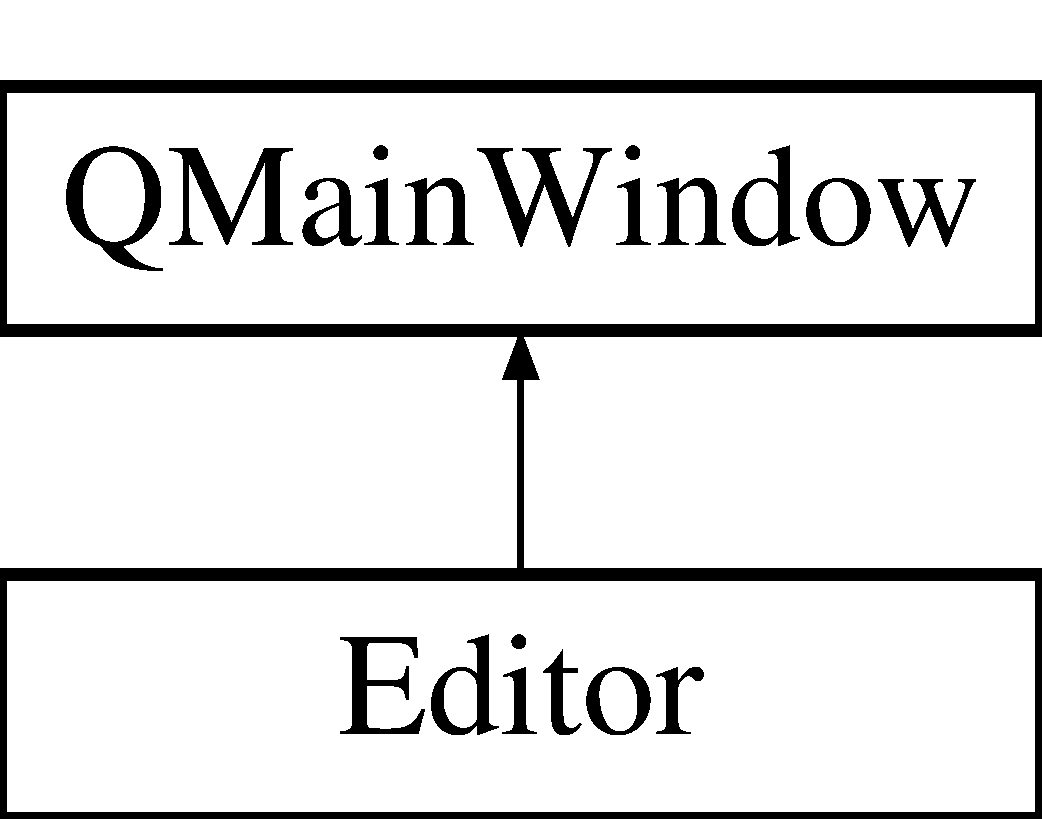
\includegraphics[height=2.000000cm]{class_editor}
\end{center}
\end{figure}
\subsection*{Public Member Functions}
\begin{DoxyCompactItemize}
\item 
\mbox{\hyperlink{class_editor_a2918aceeffbc123a96e201b0934b9b16}{Editor}} (Q\+Widget $\ast$parent=0)
\item 
void \mbox{\hyperlink{class_editor_a1641e805c7e3d2441c8658ddc9f04ed1}{create\+Map}} ()
\item 
void \mbox{\hyperlink{class_editor_add1f4b900d9c8ae6065ccd769929b617}{save\+Map}} ()
\item 
void \mbox{\hyperlink{class_editor_a392c4c8e63399e824bbac9b669287602}{load\+Map}} ()
\item 
void \mbox{\hyperlink{class_editor_a35b08c0c5641203323d8865afe4a2959}{clear\+Tree}} ()
\item 
void \mbox{\hyperlink{class_editor_a5e4c7dcadb49adcdece3235a92a5fa5c}{delete\+Map}} ()
\item 
\mbox{\Hypertarget{class_editor_ad07ccb2dbdf4d50be5fdf02543c4e904}\label{class_editor_ad07ccb2dbdf4d50be5fdf02543c4e904}} 
void {\bfseries draw\+Grid\+Layout} (int x, int y)
\item 
void \mbox{\hyperlink{class_editor_a64370ff1f5ceddcb1e261f2360ca1f82}{update\+Tree\+Number\+Of\+Tiles}} ()
\item 
void \mbox{\hyperlink{class_editor_ab6a95acaa882cf1184e5fee306bf0d60}{update\+Tree\+Number\+Of\+Obstacles}} ()
\item 
void \mbox{\hyperlink{class_editor_af7eec42c19816c227c820871cf119dac}{update\+Tree\+Map\+Size}} ()
\item 
void \mbox{\hyperlink{class_editor_af487b4d79b6a61c4613ccf605328b708}{update\+Map\+Values}} (int x, int y)
\item 
void \mbox{\hyperlink{class_editor_a90948c660641c5e416a34ecf05c134ae}{add\+Tree\+Items}} ()
\item 
void \mbox{\hyperlink{class_editor_a567769e5c55f904085a8ed615159ffd9}{add\+Tree\+Map}} (double x, double y)
\item 
\mbox{\Hypertarget{class_editor_a0b2bc4197d01bfc6c7a34645be26159e}\label{class_editor_a0b2bc4197d01bfc6c7a34645be26159e}} 
void {\bfseries set\+Tree\+Tiles\+Position} (Q\+PointF position, int index)
\item 
\mbox{\Hypertarget{class_editor_ae674ecab67ac5f3842f1af550cfe60e3}\label{class_editor_ae674ecab67ac5f3842f1af550cfe60e3}} 
void {\bfseries set\+Tree\+Obstacles\+Position} (Q\+PointF position, int index)
\item 
void \mbox{\hyperlink{class_editor_a7c91cc0098ff48ec885422b6c49d27e0}{add\+Child}} (Q\+Tree\+Widget\+Item $\ast$parent, Q\+String name, int posX, int posY)
\item 
\mbox{\Hypertarget{class_editor_a13cac52c413b63b00ff2fe780f65ba69}\label{class_editor_a13cac52c413b63b00ff2fe780f65ba69}} 
void {\bfseries connect\+Scene} ()
\item 
\mbox{\Hypertarget{class_editor_ae60e42139a89b158340861caeded5ac0}\label{class_editor_ae60e42139a89b158340861caeded5ac0}} 
void {\bfseries connect\+Tree\+Widget} ()
\item 
\mbox{\Hypertarget{class_editor_a27e06cb4821cac63581425db3e556195}\label{class_editor_a27e06cb4821cac63581425db3e556195}} 
void {\bfseries auto\+Save} ()
\item 
\mbox{\Hypertarget{class_editor_a5adfadc8dff014c5462cd71e0a2c6259}\label{class_editor_a5adfadc8dff014c5462cd71e0a2c6259}} 
void {\bfseries key\+Press\+Event} (Q\+Key\+Event $\ast$event)
\end{DoxyCompactItemize}


\subsection{Constructor \& Destructor Documentation}
\mbox{\Hypertarget{class_editor_a2918aceeffbc123a96e201b0934b9b16}\label{class_editor_a2918aceeffbc123a96e201b0934b9b16}} 
\index{Editor@{Editor}!Editor@{Editor}}
\index{Editor@{Editor}!Editor@{Editor}}
\subsubsection{\texorpdfstring{Editor()}{Editor()}}
{\footnotesize\ttfamily Editor\+::\+Editor (\begin{DoxyParamCaption}\item[{Q\+Widget $\ast$}]{parent = {\ttfamily 0} }\end{DoxyParamCaption})\hspace{0.3cm}{\ttfamily [explicit]}}

Erstellt ein Editorfenster 
\begin{DoxyParams}{Parameters}
{\em $\ast$parent} & Fenster in welchem der \mbox{\hyperlink{class_editor}{Editor}} gezeichnet werden soll \\
\hline
\end{DoxyParams}


\subsection{Member Function Documentation}
\mbox{\Hypertarget{class_editor_a7c91cc0098ff48ec885422b6c49d27e0}\label{class_editor_a7c91cc0098ff48ec885422b6c49d27e0}} 
\index{Editor@{Editor}!add\+Child@{add\+Child}}
\index{add\+Child@{add\+Child}!Editor@{Editor}}
\subsubsection{\texorpdfstring{add\+Child()}{addChild()}}
{\footnotesize\ttfamily void Editor\+::add\+Child (\begin{DoxyParamCaption}\item[{Q\+Tree\+Widget\+Item $\ast$}]{parent,  }\item[{Q\+String}]{name,  }\item[{int}]{posX,  }\item[{int}]{posY }\end{DoxyParamCaption})}

Fügt dem Tree\+View ein Kindelement hinzu. 
\begin{DoxyParams}{Parameters}
{\em $\ast$param} & zeigt auf das Tree\+View \\
\hline
{\em name} & Typ des Elementes (\mbox{\hyperlink{class_tile}{Tile}},\mbox{\hyperlink{class_obstacle}{Obstacle}}..) \\
\hline
{\em posX} & x-\/\+Position des Elementes \\
\hline
{\em posY} & y-\/\+Position des Elementes \\
\hline
\end{DoxyParams}
\mbox{\Hypertarget{class_editor_a90948c660641c5e416a34ecf05c134ae}\label{class_editor_a90948c660641c5e416a34ecf05c134ae}} 
\index{Editor@{Editor}!add\+Tree\+Items@{add\+Tree\+Items}}
\index{add\+Tree\+Items@{add\+Tree\+Items}!Editor@{Editor}}
\subsubsection{\texorpdfstring{add\+Tree\+Items()}{addTreeItems()}}
{\footnotesize\ttfamily void Editor\+::add\+Tree\+Items (\begin{DoxyParamCaption}{ }\end{DoxyParamCaption})}

Erstellt Überschriftelemente für das Tree\+View \mbox{\Hypertarget{class_editor_a567769e5c55f904085a8ed615159ffd9}\label{class_editor_a567769e5c55f904085a8ed615159ffd9}} 
\index{Editor@{Editor}!add\+Tree\+Map@{add\+Tree\+Map}}
\index{add\+Tree\+Map@{add\+Tree\+Map}!Editor@{Editor}}
\subsubsection{\texorpdfstring{add\+Tree\+Map()}{addTreeMap()}}
{\footnotesize\ttfamily void Editor\+::add\+Tree\+Map (\begin{DoxyParamCaption}\item[{double}]{x,  }\item[{double}]{y }\end{DoxyParamCaption})}

Setzt die geöffnete \mbox{\hyperlink{class_map}{Map}} als Hauptelement des Tree\+View \mbox{\Hypertarget{class_editor_a35b08c0c5641203323d8865afe4a2959}\label{class_editor_a35b08c0c5641203323d8865afe4a2959}} 
\index{Editor@{Editor}!clear\+Tree@{clear\+Tree}}
\index{clear\+Tree@{clear\+Tree}!Editor@{Editor}}
\subsubsection{\texorpdfstring{clear\+Tree()}{clearTree()}}
{\footnotesize\ttfamily void Editor\+::clear\+Tree (\begin{DoxyParamCaption}{ }\end{DoxyParamCaption})}

Löscht alle Elemente des Tree\+View \mbox{\Hypertarget{class_editor_a1641e805c7e3d2441c8658ddc9f04ed1}\label{class_editor_a1641e805c7e3d2441c8658ddc9f04ed1}} 
\index{Editor@{Editor}!create\+Map@{create\+Map}}
\index{create\+Map@{create\+Map}!Editor@{Editor}}
\subsubsection{\texorpdfstring{create\+Map()}{createMap()}}
{\footnotesize\ttfamily void Editor\+::create\+Map (\begin{DoxyParamCaption}{ }\end{DoxyParamCaption})}

Erstellt eine leere \mbox{\hyperlink{class_map}{Map}} und öffnet diese. \mbox{\Hypertarget{class_editor_a5e4c7dcadb49adcdece3235a92a5fa5c}\label{class_editor_a5e4c7dcadb49adcdece3235a92a5fa5c}} 
\index{Editor@{Editor}!delete\+Map@{delete\+Map}}
\index{delete\+Map@{delete\+Map}!Editor@{Editor}}
\subsubsection{\texorpdfstring{delete\+Map()}{deleteMap()}}
{\footnotesize\ttfamily void Editor\+::delete\+Map (\begin{DoxyParamCaption}{ }\end{DoxyParamCaption})}

Löscht die geoffnete \mbox{\hyperlink{class_map}{Map}} \mbox{\Hypertarget{class_editor_a392c4c8e63399e824bbac9b669287602}\label{class_editor_a392c4c8e63399e824bbac9b669287602}} 
\index{Editor@{Editor}!load\+Map@{load\+Map}}
\index{load\+Map@{load\+Map}!Editor@{Editor}}
\subsubsection{\texorpdfstring{load\+Map()}{loadMap()}}
{\footnotesize\ttfamily void Editor\+::load\+Map (\begin{DoxyParamCaption}{ }\end{DoxyParamCaption})}

Lädt eine Map-\/\+Datei und öffnet die \mbox{\hyperlink{class_map}{Map}} im \mbox{\hyperlink{class_editor}{Editor}} \mbox{\Hypertarget{class_editor_add1f4b900d9c8ae6065ccd769929b617}\label{class_editor_add1f4b900d9c8ae6065ccd769929b617}} 
\index{Editor@{Editor}!save\+Map@{save\+Map}}
\index{save\+Map@{save\+Map}!Editor@{Editor}}
\subsubsection{\texorpdfstring{save\+Map()}{saveMap()}}
{\footnotesize\ttfamily void Editor\+::save\+Map (\begin{DoxyParamCaption}{ }\end{DoxyParamCaption})}

Speichert die geöffnete \mbox{\hyperlink{class_map}{Map}} in einer X\+M\+L-\/\+Datei \mbox{\Hypertarget{class_editor_af487b4d79b6a61c4613ccf605328b708}\label{class_editor_af487b4d79b6a61c4613ccf605328b708}} 
\index{Editor@{Editor}!update\+Map\+Values@{update\+Map\+Values}}
\index{update\+Map\+Values@{update\+Map\+Values}!Editor@{Editor}}
\subsubsection{\texorpdfstring{update\+Map\+Values()}{updateMapValues()}}
{\footnotesize\ttfamily void Editor\+::update\+Map\+Values (\begin{DoxyParamCaption}\item[{int}]{x,  }\item[{int}]{y }\end{DoxyParamCaption})}

Ändert die Größe der \mbox{\hyperlink{class_map}{Map}} und zeichnet diese neu 
\begin{DoxyParams}{Parameters}
{\em x} & neuer x-\/\+Wert der \mbox{\hyperlink{class_map}{Map}} \\
\hline
{\em y} & neuer y-\/\+Wert der \mbox{\hyperlink{class_map}{Map}} \\
\hline
\end{DoxyParams}
\mbox{\Hypertarget{class_editor_af7eec42c19816c227c820871cf119dac}\label{class_editor_af7eec42c19816c227c820871cf119dac}} 
\index{Editor@{Editor}!update\+Tree\+Map\+Size@{update\+Tree\+Map\+Size}}
\index{update\+Tree\+Map\+Size@{update\+Tree\+Map\+Size}!Editor@{Editor}}
\subsubsection{\texorpdfstring{update\+Tree\+Map\+Size()}{updateTreeMapSize()}}
{\footnotesize\ttfamily void Editor\+::update\+Tree\+Map\+Size (\begin{DoxyParamCaption}{ }\end{DoxyParamCaption})}

Aktualisiert die Größe der \mbox{\hyperlink{class_map}{Map}} im Tree\+View \mbox{\Hypertarget{class_editor_ab6a95acaa882cf1184e5fee306bf0d60}\label{class_editor_ab6a95acaa882cf1184e5fee306bf0d60}} 
\index{Editor@{Editor}!update\+Tree\+Number\+Of\+Obstacles@{update\+Tree\+Number\+Of\+Obstacles}}
\index{update\+Tree\+Number\+Of\+Obstacles@{update\+Tree\+Number\+Of\+Obstacles}!Editor@{Editor}}
\subsubsection{\texorpdfstring{update\+Tree\+Number\+Of\+Obstacles()}{updateTreeNumberOfObstacles()}}
{\footnotesize\ttfamily void Editor\+::update\+Tree\+Number\+Of\+Obstacles (\begin{DoxyParamCaption}{ }\end{DoxyParamCaption})}

Aktualisiert die Anzahl der Obstacles im Tree\+View \mbox{\Hypertarget{class_editor_a64370ff1f5ceddcb1e261f2360ca1f82}\label{class_editor_a64370ff1f5ceddcb1e261f2360ca1f82}} 
\index{Editor@{Editor}!update\+Tree\+Number\+Of\+Tiles@{update\+Tree\+Number\+Of\+Tiles}}
\index{update\+Tree\+Number\+Of\+Tiles@{update\+Tree\+Number\+Of\+Tiles}!Editor@{Editor}}
\subsubsection{\texorpdfstring{update\+Tree\+Number\+Of\+Tiles()}{updateTreeNumberOfTiles()}}
{\footnotesize\ttfamily void Editor\+::update\+Tree\+Number\+Of\+Tiles (\begin{DoxyParamCaption}{ }\end{DoxyParamCaption})}

Aktualisiert die Anzahl der Tiles im Tree\+View 

The documentation for this class was generated from the following files\+:\begin{DoxyCompactItemize}
\item 
D\+:/swt1718-\/editor/bin/source/editor.\+h\item 
D\+:/swt1718-\/editor/bin/source/editor.\+cpp\end{DoxyCompactItemize}

\hypertarget{class_endingtile}{}\section{Endingtile Class Reference}
\label{class_endingtile}\index{Endingtile@{Endingtile}}
Inheritance diagram for Endingtile\+:\begin{figure}[H]
\begin{center}
\leavevmode
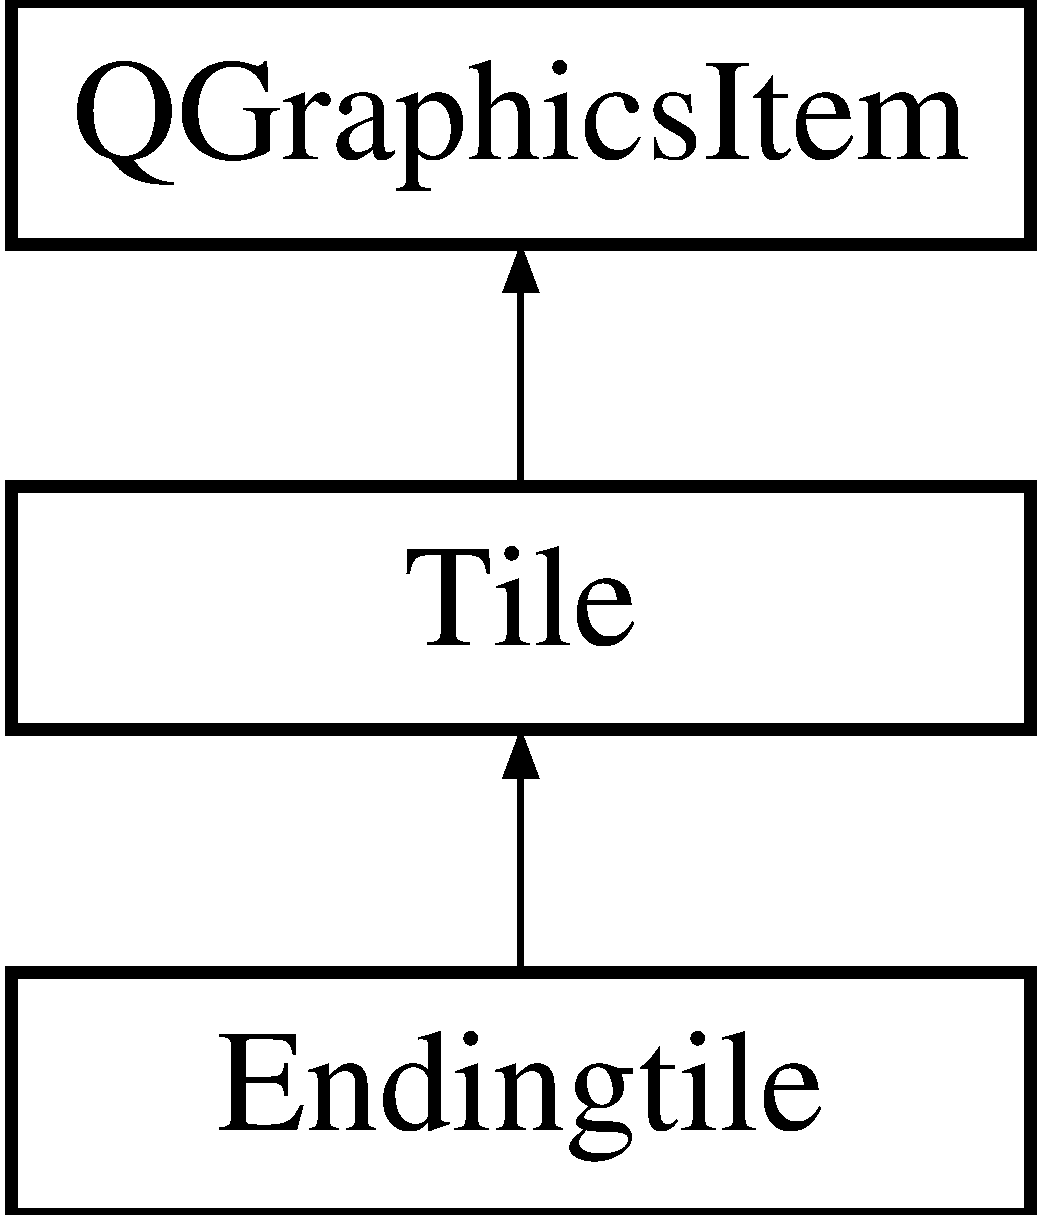
\includegraphics[height=3.000000cm]{class_endingtile}
\end{center}
\end{figure}
\subsection*{Public Member Functions}
\begin{DoxyCompactItemize}
\item 
virtual Q\+RectF \mbox{\hyperlink{class_endingtile_a96035b6213a6704c781ccde3792e04d8}{bounding\+Rect}} () const
\item 
virtual void \mbox{\hyperlink{class_endingtile_accfd225f8b68494147466d98f0eb38a3}{paint}} (Q\+Painter $\ast$painter, const Q\+Style\+Option\+Graphics\+Item $\ast$option, Q\+Widget $\ast$widget)
\item 
virtual Q\+String \mbox{\hyperlink{class_endingtile_a1e3f8d51207bd2fcd295e88b5e037b03}{get\+Type}} ()
\item 
void \mbox{\hyperlink{class_endingtile_a130af5ae1efa2bf53ffe23f89fe06834}{rotate}} ()
\end{DoxyCompactItemize}
\subsection*{Static Public Member Functions}
\begin{DoxyCompactItemize}
\item 
static \mbox{\hyperlink{class_endingtile}{Endingtile}} $\ast$ \mbox{\hyperlink{class_endingtile_aebb90e09ae669f305c980e9e7420c397}{create\+Ending\+Tile}} (int nx, int ny, double nascent, int ndirection)
\end{DoxyCompactItemize}
\subsection*{Additional Inherited Members}


\subsection{Member Function Documentation}
\mbox{\Hypertarget{class_endingtile_a96035b6213a6704c781ccde3792e04d8}\label{class_endingtile_a96035b6213a6704c781ccde3792e04d8}} 
\index{Endingtile@{Endingtile}!bounding\+Rect@{bounding\+Rect}}
\index{bounding\+Rect@{bounding\+Rect}!Endingtile@{Endingtile}}
\subsubsection{\texorpdfstring{bounding\+Rect()}{boundingRect()}}
{\footnotesize\ttfamily Q\+RectF Endingtile\+::bounding\+Rect (\begin{DoxyParamCaption}{ }\end{DoxyParamCaption}) const\hspace{0.3cm}{\ttfamily [virtual]}}

Erstellt ein Begrenzungsrechteck für das \mbox{\hyperlink{class_tile}{Tile}},Dieses wird sowohl zum zeichnen, als auch für weitere Interaktion benötigt \mbox{\Hypertarget{class_endingtile_aebb90e09ae669f305c980e9e7420c397}\label{class_endingtile_aebb90e09ae669f305c980e9e7420c397}} 
\index{Endingtile@{Endingtile}!create\+Ending\+Tile@{create\+Ending\+Tile}}
\index{create\+Ending\+Tile@{create\+Ending\+Tile}!Endingtile@{Endingtile}}
\subsubsection{\texorpdfstring{create\+Ending\+Tile()}{createEndingTile()}}
{\footnotesize\ttfamily \mbox{\hyperlink{class_endingtile}{Endingtile}} $\ast$ Endingtile\+::create\+Ending\+Tile (\begin{DoxyParamCaption}\item[{int}]{nx,  }\item[{int}]{ny,  }\item[{double}]{nascent,  }\item[{int}]{ndirection }\end{DoxyParamCaption})\hspace{0.3cm}{\ttfamily [static]}}

Prüft ob die \mbox{\hyperlink{class_map}{Map}} schon einen Endabschnitt hat, falls nicht, wird einer Erzeugt \begin{DoxyReturn}{Returns}
Pointer der auf den Endabschnitt zeigt 
\end{DoxyReturn}
\mbox{\Hypertarget{class_endingtile_a1e3f8d51207bd2fcd295e88b5e037b03}\label{class_endingtile_a1e3f8d51207bd2fcd295e88b5e037b03}} 
\index{Endingtile@{Endingtile}!get\+Type@{get\+Type}}
\index{get\+Type@{get\+Type}!Endingtile@{Endingtile}}
\subsubsection{\texorpdfstring{get\+Type()}{getType()}}
{\footnotesize\ttfamily Q\+String Endingtile\+::get\+Type (\begin{DoxyParamCaption}{ }\end{DoxyParamCaption})\hspace{0.3cm}{\ttfamily [virtual]}}

Gibt den Typen des \mbox{\hyperlink{class_tile}{Tile}} zurück \begin{DoxyReturn}{Returns}
Typ des \mbox{\hyperlink{class_tile}{Tile}} 
\end{DoxyReturn}


Reimplemented from \mbox{\hyperlink{class_tile_ad1dbea94d96060491a2dc4c7b92b31ab}{Tile}}.

\mbox{\Hypertarget{class_endingtile_accfd225f8b68494147466d98f0eb38a3}\label{class_endingtile_accfd225f8b68494147466d98f0eb38a3}} 
\index{Endingtile@{Endingtile}!paint@{paint}}
\index{paint@{paint}!Endingtile@{Endingtile}}
\subsubsection{\texorpdfstring{paint()}{paint()}}
{\footnotesize\ttfamily void Endingtile\+::paint (\begin{DoxyParamCaption}\item[{Q\+Painter $\ast$}]{painter,  }\item[{const Q\+Style\+Option\+Graphics\+Item $\ast$}]{option,  }\item[{Q\+Widget $\ast$}]{widget }\end{DoxyParamCaption})\hspace{0.3cm}{\ttfamily [virtual]}}

Zeichnet das \mbox{\hyperlink{class_tile}{Tile}} 
\begin{DoxyParams}{Parameters}
{\em painter} & Painter der zum Zeichnen benutzt wird \\
\hline
{\em option} & Optionen für das Zeichnen \\
\hline
{\em widget} & Widget in welches gezeichnet wird \\
\hline
\end{DoxyParams}


Reimplemented from \mbox{\hyperlink{class_tile_ab0a7262b6fab842a7a467fcb2f7592eb}{Tile}}.

\mbox{\Hypertarget{class_endingtile_a130af5ae1efa2bf53ffe23f89fe06834}\label{class_endingtile_a130af5ae1efa2bf53ffe23f89fe06834}} 
\index{Endingtile@{Endingtile}!rotate@{rotate}}
\index{rotate@{rotate}!Endingtile@{Endingtile}}
\subsubsection{\texorpdfstring{rotate()}{rotate()}}
{\footnotesize\ttfamily void Endingtile\+::rotate (\begin{DoxyParamCaption}{ }\end{DoxyParamCaption})\hspace{0.3cm}{\ttfamily [virtual]}}

Rotiert das \mbox{\hyperlink{class_tile}{Tile}} 

Reimplemented from \mbox{\hyperlink{class_tile_a15c3d8260c8950d3461e3ba2849cd141}{Tile}}.



The documentation for this class was generated from the following files\+:\begin{DoxyCompactItemize}
\item 
D\+:/swt1718-\/editor/bin/source/endingtile.\+h\item 
D\+:/swt1718-\/editor/bin/source/endingtile.\+cpp\end{DoxyCompactItemize}

\hypertarget{class_intersection}{}\section{Intersection Class Reference}
\label{class_intersection}\index{Intersection@{Intersection}}
Inheritance diagram for Intersection\+:\begin{figure}[H]
\begin{center}
\leavevmode
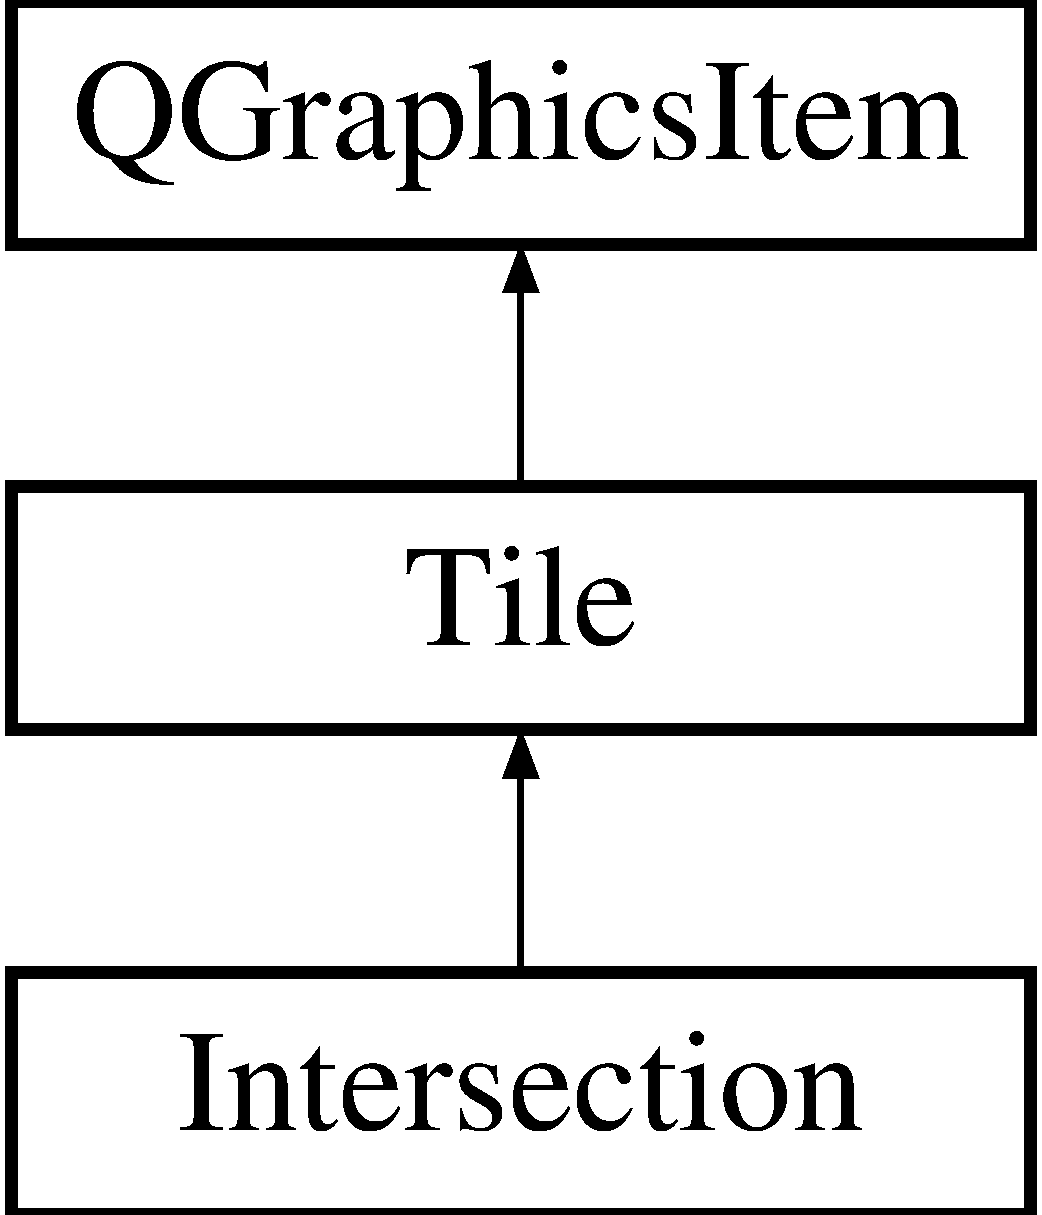
\includegraphics[height=3.000000cm]{class_intersection}
\end{center}
\end{figure}
\subsection*{Public Member Functions}
\begin{DoxyCompactItemize}
\item 
\mbox{\hyperlink{class_intersection_ae877f46e9471e82f16ff180c41e1490a}{Intersection}} (double x, double y, double ascent)
\item 
Q\+RectF \mbox{\hyperlink{class_intersection_a0d96ac4dc6971a4a99ab652b7f15ed41}{bounding\+Rect}} () const
\item 
Q\+String \mbox{\hyperlink{class_intersection_a8bed77f9049accb2dcc50c3e961f5143}{get\+Type}} ()
\item 
void \mbox{\hyperlink{class_intersection_aa9e14b51410964e0ce66b1762bec252a}{paint}} (Q\+Painter $\ast$painter, const Q\+Style\+Option\+Graphics\+Item $\ast$option, Q\+Widget $\ast$widget)
\end{DoxyCompactItemize}
\subsection*{Additional Inherited Members}


\subsection{Constructor \& Destructor Documentation}
\mbox{\Hypertarget{class_intersection_ae877f46e9471e82f16ff180c41e1490a}\label{class_intersection_ae877f46e9471e82f16ff180c41e1490a}} 
\index{Intersection@{Intersection}!Intersection@{Intersection}}
\index{Intersection@{Intersection}!Intersection@{Intersection}}
\subsubsection{\texorpdfstring{Intersection()}{Intersection()}}
{\footnotesize\ttfamily Intersection\+::\+Intersection (\begin{DoxyParamCaption}\item[{double}]{x,  }\item[{double}]{y,  }\item[{double}]{ascent }\end{DoxyParamCaption})}

Erstellt eine Kreuzung und fügt diese dem \mbox{\hyperlink{class_editor}{Editor}} hinzu 
\begin{DoxyParams}{Parameters}
{\em x} & x-\/\+Koordinate der Kreuzung \\
\hline
{\em y} & y-\/\+Koordinate der Kreuzung \\
\hline
{\em ascent} & Steigung der Kreuzung \\
\hline
\end{DoxyParams}


\subsection{Member Function Documentation}
\mbox{\Hypertarget{class_intersection_a0d96ac4dc6971a4a99ab652b7f15ed41}\label{class_intersection_a0d96ac4dc6971a4a99ab652b7f15ed41}} 
\index{Intersection@{Intersection}!bounding\+Rect@{bounding\+Rect}}
\index{bounding\+Rect@{bounding\+Rect}!Intersection@{Intersection}}
\subsubsection{\texorpdfstring{bounding\+Rect()}{boundingRect()}}
{\footnotesize\ttfamily Q\+RectF Intersection\+::bounding\+Rect (\begin{DoxyParamCaption}{ }\end{DoxyParamCaption}) const}

Erstellt ein Begrenzungsrechteck für das \mbox{\hyperlink{class_tile}{Tile}},Dieses wird sowohl zum zeichnen, als auch für weitere Interaktion benötigt \mbox{\Hypertarget{class_intersection_a8bed77f9049accb2dcc50c3e961f5143}\label{class_intersection_a8bed77f9049accb2dcc50c3e961f5143}} 
\index{Intersection@{Intersection}!get\+Type@{get\+Type}}
\index{get\+Type@{get\+Type}!Intersection@{Intersection}}
\subsubsection{\texorpdfstring{get\+Type()}{getType()}}
{\footnotesize\ttfamily Q\+String Intersection\+::get\+Type (\begin{DoxyParamCaption}{ }\end{DoxyParamCaption})\hspace{0.3cm}{\ttfamily [virtual]}}

Gibt den Typen des \mbox{\hyperlink{class_tile}{Tile}} zurück \begin{DoxyReturn}{Returns}
Typ des \mbox{\hyperlink{class_tile}{Tile}} 
\end{DoxyReturn}


Reimplemented from \mbox{\hyperlink{class_tile_ad1dbea94d96060491a2dc4c7b92b31ab}{Tile}}.

\mbox{\Hypertarget{class_intersection_aa9e14b51410964e0ce66b1762bec252a}\label{class_intersection_aa9e14b51410964e0ce66b1762bec252a}} 
\index{Intersection@{Intersection}!paint@{paint}}
\index{paint@{paint}!Intersection@{Intersection}}
\subsubsection{\texorpdfstring{paint()}{paint()}}
{\footnotesize\ttfamily void Intersection\+::paint (\begin{DoxyParamCaption}\item[{Q\+Painter $\ast$}]{painter,  }\item[{const Q\+Style\+Option\+Graphics\+Item $\ast$}]{option,  }\item[{Q\+Widget $\ast$}]{widget }\end{DoxyParamCaption})\hspace{0.3cm}{\ttfamily [virtual]}}

Zeichnet das \mbox{\hyperlink{class_tile}{Tile}} 
\begin{DoxyParams}{Parameters}
{\em painter} & Painter der zum Zeichnen benutzt wird \\
\hline
{\em option} & Optionen für das Zeichnen \\
\hline
{\em widget} & Widget in welches gezeichnet wird \\
\hline
\end{DoxyParams}


Reimplemented from \mbox{\hyperlink{class_tile_ab0a7262b6fab842a7a467fcb2f7592eb}{Tile}}.



The documentation for this class was generated from the following files\+:\begin{DoxyCompactItemize}
\item 
D\+:/swt1718-\/editor/bin/source/intersection.\+h\item 
D\+:/swt1718-\/editor/bin/source/intersection.\+cpp\end{DoxyCompactItemize}

\hypertarget{class_map}{}\section{Map Class Reference}
\label{class_map}\index{Map@{Map}}


{\ttfamily \#include $<$map.\+h$>$}

\subsection*{Public Member Functions}
\begin{DoxyCompactItemize}
\item 
\mbox{\hyperlink{class_map_a0f5ad0fd4563497b4214038cbca8b582}{Map}} ()
\item 
\mbox{\hyperlink{class_map_a7dd574b3746a45123fd765945b6a2a7e}{Map}} (int x, int y)
\item 
\mbox{\hyperlink{class_map_aa403fbe09394ccf39747588f5168e3b2}{$\sim$\+Map}} ()
\item 
\mbox{\hyperlink{class_tile}{Tile}} $\ast$ \mbox{\hyperlink{class_map_a60bdbaac9468f1ceb427e38db3eb46a0}{get\+Tile}} (int i)
\item 
\mbox{\hyperlink{class_tile}{Tile}} $\ast$ \mbox{\hyperlink{class_map_aa84b261dd360a64ef6fadfb4c4b1f2ff}{get\+Current\+Tile}} ()
\item 
\mbox{\hyperlink{class_obstacle}{Obstacle}} $\ast$ \mbox{\hyperlink{class_map_a17453848c1ade655219c73c15a9b1b78}{get\+Obstacle}} (int i)
\item 
\mbox{\hyperlink{class_obstacle}{Obstacle}} $\ast$ \mbox{\hyperlink{class_map_a61b2390d5a19071bf3509152872f5ac6}{get\+Current\+Obstacle}} ()
\item 
\mbox{\Hypertarget{class_map_a6ad7382f42482e46415124c5af3b9c33}\label{class_map_a6ad7382f42482e46415124c5af3b9c33}} 
\mbox{\hyperlink{class_tile}{Tile}} $\ast$ {\bfseries get\+Starting\+Tile} ()
\item 
\mbox{\Hypertarget{class_map_a4e5e1640f6520226491b06490f624eb6}\label{class_map_a4e5e1640f6520226491b06490f624eb6}} 
\mbox{\hyperlink{class_tile}{Tile}} $\ast$ {\bfseries get\+Ending\+Tile} ()
\item 
\mbox{\Hypertarget{class_map_a941f348abe63fb43c8a912500a61f2f6}\label{class_map_a941f348abe63fb43c8a912500a61f2f6}} 
void {\bfseries set\+Starting\+Tile} (\mbox{\hyperlink{class_tile}{Tile}} $\ast$t)
\item 
\mbox{\Hypertarget{class_map_a88b6d85703a92e96963e6dc6a8042521}\label{class_map_a88b6d85703a92e96963e6dc6a8042521}} 
void {\bfseries set\+Ending\+Tile} (\mbox{\hyperlink{class_tile}{Tile}} $\ast$t)
\item 
void \mbox{\hyperlink{class_map_ab4fe2e5f95e7fd16f028a0ffe1db8917}{set\+Starting\+Point}} (int x, int y)
\item 
void \mbox{\hyperlink{class_map_aedbdf210bf5ec2b87fa834e8e20b16dd}{set\+Ending\+Point}} (int x, int y)
\item 
void \mbox{\hyperlink{class_map_a483c836df20db96ba2f7118f7b3c2dfd}{set\+Size}} (int x, int y)
\item 
void \mbox{\hyperlink{class_map_a2727714e173313a9b2738b34deb78fb7}{add\+Tile}} (\mbox{\hyperlink{class_tile}{Tile}} $\ast$t)
\item 
void \mbox{\hyperlink{class_map_adf099f25e89a3470a348ccf87bc4a55d}{add\+Obstacle}} (\mbox{\hyperlink{class_obstacle}{Obstacle}} $\ast$o)
\item 
void \mbox{\hyperlink{class_map_aa220ee8afb6eb77ae41d137d44919173}{delete\+Tile}} (int i)
\item 
void \mbox{\hyperlink{class_map_aaad5b40b9c748b23da1cb3420e0c86de}{delete\+Obstacle}} (int i)
\item 
void \mbox{\hyperlink{class_map_a89bab8e9b24c94b2696d624dac43cffa}{delete\+Current\+Tile}} ()
\item 
void \mbox{\hyperlink{class_map_ac29cdcf87495d5335655ab55f890a57e}{delete\+Current\+Obstacle}} ()
\item 
Q\+PointF \mbox{\hyperlink{class_map_a378b0d0c136bd92b080d206f3bc2cd00}{get\+Starting\+Point}} ()
\item 
Q\+PointF \mbox{\hyperlink{class_map_a89f8852e818ad3c4ff7ff3ff9434e544}{get\+Ending\+Point}} ()
\item 
unsigned int \mbox{\hyperlink{class_map_ae993424a64bb5638db33127d2a450014}{get\+Number\+Of\+Tiles}} ()
\item 
unsigned int \mbox{\hyperlink{class_map_a2314b59099da9d9fdd16e9f816150709}{get\+Number\+Of\+Obstacles}} ()
\item 
unsigned int \mbox{\hyperlink{class_map_af960a5f3d085679f49fc56b0cc0ffdaf}{get\+Number\+Of\+Items}} ()
\item 
unsigned int \mbox{\hyperlink{class_map_a295543a6b7ade2cdffd2faba2adda417}{get\+SizeX}} ()
\item 
unsigned int \mbox{\hyperlink{class_map_a07c437bb06a96676d6a732a559d3df4f}{get\+SizeY}} ()
\item 
int \mbox{\hyperlink{class_map_aced3d71b8481cf37e218ff4ddb987874}{get\+Grid\+Size}} ()
\item 
void \mbox{\hyperlink{class_map_a575b2a270c179acb59b5809b4fa1dfeb}{set\+Map\+Path}} ()
\item 
Q\+Painter\+Path \mbox{\hyperlink{class_map_ada28e2fd173999bcf7981d55de145d6d}{get\+Map\+Path}} ()
\item 
\mbox{\Hypertarget{class_map_aa043caa073487984ab260266249fad44}\label{class_map_aa043caa073487984ab260266249fad44}} 
\mbox{\hyperlink{class_memento}{Memento}} $\ast$ {\bfseries create\+Memento} ()
\item 
\mbox{\Hypertarget{class_map_aa8d2945eaaf81e9f12122c4a65b02e73}\label{class_map_aa8d2945eaaf81e9f12122c4a65b02e73}} 
void {\bfseries set\+Memento} (\mbox{\hyperlink{class_memento}{Memento}} $\ast$m)
\end{DoxyCompactItemize}


\subsection{Detailed Description}
Speichert die relevanten Daten einer \mbox{\hyperlink{class_map}{Map}} und erlaubt das hinzufügen und bearbeiten von Elementen auf dieser 

\subsection{Constructor \& Destructor Documentation}
\mbox{\Hypertarget{class_map_a0f5ad0fd4563497b4214038cbca8b582}\label{class_map_a0f5ad0fd4563497b4214038cbca8b582}} 
\index{Map@{Map}!Map@{Map}}
\index{Map@{Map}!Map@{Map}}
\subsubsection{\texorpdfstring{Map()}{Map()}\hspace{0.1cm}{\footnotesize\ttfamily [1/2]}}
{\footnotesize\ttfamily Map\+::\+Map (\begin{DoxyParamCaption}{ }\end{DoxyParamCaption})}

Erstellt eine \mbox{\hyperlink{class_map}{Map}} der größe 0 \mbox{\Hypertarget{class_map_a7dd574b3746a45123fd765945b6a2a7e}\label{class_map_a7dd574b3746a45123fd765945b6a2a7e}} 
\index{Map@{Map}!Map@{Map}}
\index{Map@{Map}!Map@{Map}}
\subsubsection{\texorpdfstring{Map()}{Map()}\hspace{0.1cm}{\footnotesize\ttfamily [2/2]}}
{\footnotesize\ttfamily Map\+::\+Map (\begin{DoxyParamCaption}\item[{int}]{x,  }\item[{int}]{y }\end{DoxyParamCaption})}

Erstellt eine leere \mbox{\hyperlink{class_map}{Map}} 
\begin{DoxyParams}{Parameters}
{\em x} & Größe der \mbox{\hyperlink{class_map}{Map}} in x-\/\+Richtung \\
\hline
{\em y} & Größe der \mbox{\hyperlink{class_map}{Map}} in y-\/\+Richtung \\
\hline
\end{DoxyParams}
\mbox{\Hypertarget{class_map_aa403fbe09394ccf39747588f5168e3b2}\label{class_map_aa403fbe09394ccf39747588f5168e3b2}} 
\index{Map@{Map}!````~Map@{$\sim$\+Map}}
\index{````~Map@{$\sim$\+Map}!Map@{Map}}
\subsubsection{\texorpdfstring{$\sim$\+Map()}{~Map()}}
{\footnotesize\ttfamily Map\+::$\sim$\+Map (\begin{DoxyParamCaption}{ }\end{DoxyParamCaption})}

Destruktor für die \mbox{\hyperlink{class_map}{Map}}. Es werden erst alle Elememte auf der \mbox{\hyperlink{class_map}{Map}} gelöscht, dann die \mbox{\hyperlink{class_map}{Map}} selbst 

\subsection{Member Function Documentation}
\mbox{\Hypertarget{class_map_adf099f25e89a3470a348ccf87bc4a55d}\label{class_map_adf099f25e89a3470a348ccf87bc4a55d}} 
\index{Map@{Map}!add\+Obstacle@{add\+Obstacle}}
\index{add\+Obstacle@{add\+Obstacle}!Map@{Map}}
\subsubsection{\texorpdfstring{add\+Obstacle()}{addObstacle()}}
{\footnotesize\ttfamily void Map\+::add\+Obstacle (\begin{DoxyParamCaption}\item[{\mbox{\hyperlink{class_obstacle}{Obstacle}} $\ast$}]{o }\end{DoxyParamCaption})}

Fügt ein \mbox{\hyperlink{class_obstacle}{Obstacle}} dem Obstacle-\/\+Vektor hinzu 
\begin{DoxyParams}{Parameters}
{\em o} & \mbox{\hyperlink{class_obstacle}{Obstacle}}, welches hinzugefügt wird \\
\hline
\end{DoxyParams}
\mbox{\Hypertarget{class_map_a2727714e173313a9b2738b34deb78fb7}\label{class_map_a2727714e173313a9b2738b34deb78fb7}} 
\index{Map@{Map}!add\+Tile@{add\+Tile}}
\index{add\+Tile@{add\+Tile}!Map@{Map}}
\subsubsection{\texorpdfstring{add\+Tile()}{addTile()}}
{\footnotesize\ttfamily void Map\+::add\+Tile (\begin{DoxyParamCaption}\item[{\mbox{\hyperlink{class_tile}{Tile}} $\ast$}]{t }\end{DoxyParamCaption})}

Fügt ein \mbox{\hyperlink{class_tile}{Tile}} dem Tile-\/\+Vektor hinzu 
\begin{DoxyParams}{Parameters}
{\em t} & \mbox{\hyperlink{class_tile}{Tile}}, welches hinzugefügt wird \\
\hline
\end{DoxyParams}
\mbox{\Hypertarget{class_map_ac29cdcf87495d5335655ab55f890a57e}\label{class_map_ac29cdcf87495d5335655ab55f890a57e}} 
\index{Map@{Map}!delete\+Current\+Obstacle@{delete\+Current\+Obstacle}}
\index{delete\+Current\+Obstacle@{delete\+Current\+Obstacle}!Map@{Map}}
\subsubsection{\texorpdfstring{delete\+Current\+Obstacle()}{deleteCurrentObstacle()}}
{\footnotesize\ttfamily void Map\+::delete\+Current\+Obstacle (\begin{DoxyParamCaption}{ }\end{DoxyParamCaption})}

Löscht das letzte erstellte \mbox{\hyperlink{class_obstacle}{Obstacle}} \mbox{\Hypertarget{class_map_a89bab8e9b24c94b2696d624dac43cffa}\label{class_map_a89bab8e9b24c94b2696d624dac43cffa}} 
\index{Map@{Map}!delete\+Current\+Tile@{delete\+Current\+Tile}}
\index{delete\+Current\+Tile@{delete\+Current\+Tile}!Map@{Map}}
\subsubsection{\texorpdfstring{delete\+Current\+Tile()}{deleteCurrentTile()}}
{\footnotesize\ttfamily void Map\+::delete\+Current\+Tile (\begin{DoxyParamCaption}{ }\end{DoxyParamCaption})}

Löscht das letzte erstellte \mbox{\hyperlink{class_tile}{Tile}} \mbox{\Hypertarget{class_map_aaad5b40b9c748b23da1cb3420e0c86de}\label{class_map_aaad5b40b9c748b23da1cb3420e0c86de}} 
\index{Map@{Map}!delete\+Obstacle@{delete\+Obstacle}}
\index{delete\+Obstacle@{delete\+Obstacle}!Map@{Map}}
\subsubsection{\texorpdfstring{delete\+Obstacle()}{deleteObstacle()}}
{\footnotesize\ttfamily void Map\+::delete\+Obstacle (\begin{DoxyParamCaption}\item[{int}]{i }\end{DoxyParamCaption})}

Löscht ein gewähltes \mbox{\hyperlink{class_obstacle}{Obstacle}} 
\begin{DoxyParams}{Parameters}
{\em i} & Position des Obstacles im Obstacle-\/\+Vektor \\
\hline
\end{DoxyParams}
\mbox{\Hypertarget{class_map_aa220ee8afb6eb77ae41d137d44919173}\label{class_map_aa220ee8afb6eb77ae41d137d44919173}} 
\index{Map@{Map}!delete\+Tile@{delete\+Tile}}
\index{delete\+Tile@{delete\+Tile}!Map@{Map}}
\subsubsection{\texorpdfstring{delete\+Tile()}{deleteTile()}}
{\footnotesize\ttfamily void Map\+::delete\+Tile (\begin{DoxyParamCaption}\item[{int}]{i }\end{DoxyParamCaption})}

Löscht ein gewähltes \mbox{\hyperlink{class_tile}{Tile}} 
\begin{DoxyParams}{Parameters}
{\em i} & Position des Tiles im Tile-\/\+Vektor \\
\hline
\end{DoxyParams}
\mbox{\Hypertarget{class_map_a61b2390d5a19071bf3509152872f5ac6}\label{class_map_a61b2390d5a19071bf3509152872f5ac6}} 
\index{Map@{Map}!get\+Current\+Obstacle@{get\+Current\+Obstacle}}
\index{get\+Current\+Obstacle@{get\+Current\+Obstacle}!Map@{Map}}
\subsubsection{\texorpdfstring{get\+Current\+Obstacle()}{getCurrentObstacle()}}
{\footnotesize\ttfamily \mbox{\hyperlink{class_obstacle}{Obstacle}} $\ast$ Map\+::get\+Current\+Obstacle (\begin{DoxyParamCaption}{ }\end{DoxyParamCaption})}

Gibt das letzte erstellte \mbox{\hyperlink{class_obstacle}{Obstacle}} zurück \begin{DoxyReturn}{Returns}
\mbox{\hyperlink{class_obstacle}{Obstacle}},welches zuletzt erstellt wurde 
\end{DoxyReturn}
\mbox{\Hypertarget{class_map_aa84b261dd360a64ef6fadfb4c4b1f2ff}\label{class_map_aa84b261dd360a64ef6fadfb4c4b1f2ff}} 
\index{Map@{Map}!get\+Current\+Tile@{get\+Current\+Tile}}
\index{get\+Current\+Tile@{get\+Current\+Tile}!Map@{Map}}
\subsubsection{\texorpdfstring{get\+Current\+Tile()}{getCurrentTile()}}
{\footnotesize\ttfamily \mbox{\hyperlink{class_tile}{Tile}} $\ast$ Map\+::get\+Current\+Tile (\begin{DoxyParamCaption}{ }\end{DoxyParamCaption})}

Gibt das letzte erstellte \mbox{\hyperlink{class_tile}{Tile}} zurück \begin{DoxyReturn}{Returns}
\mbox{\hyperlink{class_tile}{Tile}}, welches zuletzt erstellt wurde 
\end{DoxyReturn}
\mbox{\Hypertarget{class_map_a89f8852e818ad3c4ff7ff3ff9434e544}\label{class_map_a89f8852e818ad3c4ff7ff3ff9434e544}} 
\index{Map@{Map}!get\+Ending\+Point@{get\+Ending\+Point}}
\index{get\+Ending\+Point@{get\+Ending\+Point}!Map@{Map}}
\subsubsection{\texorpdfstring{get\+Ending\+Point()}{getEndingPoint()}}
{\footnotesize\ttfamily Q\+PointF Map\+::get\+Ending\+Point (\begin{DoxyParamCaption}{ }\end{DoxyParamCaption})}

Gibt den Endpunkt des autonomen Fahrzeugs zurück \begin{DoxyReturn}{Returns}
Endpunkt des Fahrzeuges 
\end{DoxyReturn}
\mbox{\Hypertarget{class_map_aced3d71b8481cf37e218ff4ddb987874}\label{class_map_aced3d71b8481cf37e218ff4ddb987874}} 
\index{Map@{Map}!get\+Grid\+Size@{get\+Grid\+Size}}
\index{get\+Grid\+Size@{get\+Grid\+Size}!Map@{Map}}
\subsubsection{\texorpdfstring{get\+Grid\+Size()}{getGridSize()}}
{\footnotesize\ttfamily int Map\+::get\+Grid\+Size (\begin{DoxyParamCaption}{ }\end{DoxyParamCaption})}

Gibt die Rastergröße der \mbox{\hyperlink{class_map}{Map}} zurück \begin{DoxyReturn}{Returns}
Rastergröße der \mbox{\hyperlink{class_map}{Map}} 
\end{DoxyReturn}
\mbox{\Hypertarget{class_map_ada28e2fd173999bcf7981d55de145d6d}\label{class_map_ada28e2fd173999bcf7981d55de145d6d}} 
\index{Map@{Map}!get\+Map\+Path@{get\+Map\+Path}}
\index{get\+Map\+Path@{get\+Map\+Path}!Map@{Map}}
\subsubsection{\texorpdfstring{get\+Map\+Path()}{getMapPath()}}
{\footnotesize\ttfamily Q\+Painter\+Path Map\+::get\+Map\+Path (\begin{DoxyParamCaption}{ }\end{DoxyParamCaption})}

Gibt die Begrenzungen der \mbox{\hyperlink{class_map}{Map}} zurück \mbox{\Hypertarget{class_map_af960a5f3d085679f49fc56b0cc0ffdaf}\label{class_map_af960a5f3d085679f49fc56b0cc0ffdaf}} 
\index{Map@{Map}!get\+Number\+Of\+Items@{get\+Number\+Of\+Items}}
\index{get\+Number\+Of\+Items@{get\+Number\+Of\+Items}!Map@{Map}}
\subsubsection{\texorpdfstring{get\+Number\+Of\+Items()}{getNumberOfItems()}}
{\footnotesize\ttfamily unsigned int Map\+::get\+Number\+Of\+Items (\begin{DoxyParamCaption}{ }\end{DoxyParamCaption})}

Gibt die Gesamtanzahl der Elemente auf der \mbox{\hyperlink{class_map}{Map}} zurück \begin{DoxyReturn}{Returns}
Gesamtzahl = Anzahl der Tiles + Anzahl der Obstacles +... 
\end{DoxyReturn}
\mbox{\Hypertarget{class_map_a2314b59099da9d9fdd16e9f816150709}\label{class_map_a2314b59099da9d9fdd16e9f816150709}} 
\index{Map@{Map}!get\+Number\+Of\+Obstacles@{get\+Number\+Of\+Obstacles}}
\index{get\+Number\+Of\+Obstacles@{get\+Number\+Of\+Obstacles}!Map@{Map}}
\subsubsection{\texorpdfstring{get\+Number\+Of\+Obstacles()}{getNumberOfObstacles()}}
{\footnotesize\ttfamily unsigned int Map\+::get\+Number\+Of\+Obstacles (\begin{DoxyParamCaption}{ }\end{DoxyParamCaption})}

Gibt die Anzahl der Obstacles auf der \mbox{\hyperlink{class_map}{Map}} zurück \begin{DoxyReturn}{Returns}
Anzahl der Obstacles auf der \mbox{\hyperlink{class_map}{Map}} 
\end{DoxyReturn}
\mbox{\Hypertarget{class_map_ae993424a64bb5638db33127d2a450014}\label{class_map_ae993424a64bb5638db33127d2a450014}} 
\index{Map@{Map}!get\+Number\+Of\+Tiles@{get\+Number\+Of\+Tiles}}
\index{get\+Number\+Of\+Tiles@{get\+Number\+Of\+Tiles}!Map@{Map}}
\subsubsection{\texorpdfstring{get\+Number\+Of\+Tiles()}{getNumberOfTiles()}}
{\footnotesize\ttfamily unsigned int Map\+::get\+Number\+Of\+Tiles (\begin{DoxyParamCaption}{ }\end{DoxyParamCaption})}

Gibt die Anzahl der Tiles auf der \mbox{\hyperlink{class_map}{Map}} zurück \begin{DoxyReturn}{Returns}
Anzahl der Tiles auf der \mbox{\hyperlink{class_map}{Map}} 
\end{DoxyReturn}
\mbox{\Hypertarget{class_map_a17453848c1ade655219c73c15a9b1b78}\label{class_map_a17453848c1ade655219c73c15a9b1b78}} 
\index{Map@{Map}!get\+Obstacle@{get\+Obstacle}}
\index{get\+Obstacle@{get\+Obstacle}!Map@{Map}}
\subsubsection{\texorpdfstring{get\+Obstacle()}{getObstacle()}}
{\footnotesize\ttfamily \mbox{\hyperlink{class_obstacle}{Obstacle}} $\ast$ Map\+::get\+Obstacle (\begin{DoxyParamCaption}\item[{int}]{i }\end{DoxyParamCaption})}

Gibt gewähltes \mbox{\hyperlink{class_obstacle}{Obstacle}} zurück 
\begin{DoxyParams}{Parameters}
{\em i} & Position des Obstacles im Obstacle-\/\+Vektor \\
\hline
\end{DoxyParams}
\begin{DoxyReturn}{Returns}
\mbox{\hyperlink{class_obstacle}{Obstacle}} an Position i im Obstacle-\/\+Vektor 
\end{DoxyReturn}
\mbox{\Hypertarget{class_map_a295543a6b7ade2cdffd2faba2adda417}\label{class_map_a295543a6b7ade2cdffd2faba2adda417}} 
\index{Map@{Map}!get\+SizeX@{get\+SizeX}}
\index{get\+SizeX@{get\+SizeX}!Map@{Map}}
\subsubsection{\texorpdfstring{get\+Size\+X()}{getSizeX()}}
{\footnotesize\ttfamily unsigned int Map\+::get\+SizeX (\begin{DoxyParamCaption}{ }\end{DoxyParamCaption})}

Gibt die Größe in x-\/\+Richtung der \mbox{\hyperlink{class_map}{Map}} zurück \begin{DoxyReturn}{Returns}
Größe der \mbox{\hyperlink{class_map}{Map}} in x-\/\+Richtung 
\end{DoxyReturn}
\mbox{\Hypertarget{class_map_a07c437bb06a96676d6a732a559d3df4f}\label{class_map_a07c437bb06a96676d6a732a559d3df4f}} 
\index{Map@{Map}!get\+SizeY@{get\+SizeY}}
\index{get\+SizeY@{get\+SizeY}!Map@{Map}}
\subsubsection{\texorpdfstring{get\+Size\+Y()}{getSizeY()}}
{\footnotesize\ttfamily unsigned int Map\+::get\+SizeY (\begin{DoxyParamCaption}{ }\end{DoxyParamCaption})}

Gibt die Größe in y-\/\+Richtung der \mbox{\hyperlink{class_map}{Map}} zurück \begin{DoxyReturn}{Returns}
Größe der \mbox{\hyperlink{class_map}{Map}} in y-\/\+Richtung 
\end{DoxyReturn}
\mbox{\Hypertarget{class_map_a378b0d0c136bd92b080d206f3bc2cd00}\label{class_map_a378b0d0c136bd92b080d206f3bc2cd00}} 
\index{Map@{Map}!get\+Starting\+Point@{get\+Starting\+Point}}
\index{get\+Starting\+Point@{get\+Starting\+Point}!Map@{Map}}
\subsubsection{\texorpdfstring{get\+Starting\+Point()}{getStartingPoint()}}
{\footnotesize\ttfamily Q\+PointF Map\+::get\+Starting\+Point (\begin{DoxyParamCaption}{ }\end{DoxyParamCaption})}

Gibt den Startpunkt des autonomen Fahrzeugs zurück \begin{DoxyReturn}{Returns}
Startpunkt des Fahrzeuges 
\end{DoxyReturn}
\mbox{\Hypertarget{class_map_a60bdbaac9468f1ceb427e38db3eb46a0}\label{class_map_a60bdbaac9468f1ceb427e38db3eb46a0}} 
\index{Map@{Map}!get\+Tile@{get\+Tile}}
\index{get\+Tile@{get\+Tile}!Map@{Map}}
\subsubsection{\texorpdfstring{get\+Tile()}{getTile()}}
{\footnotesize\ttfamily \mbox{\hyperlink{class_tile}{Tile}} $\ast$ Map\+::get\+Tile (\begin{DoxyParamCaption}\item[{int}]{i }\end{DoxyParamCaption})}

Gibt gewähltes \mbox{\hyperlink{class_tile}{Tile}} zurück 
\begin{DoxyParams}{Parameters}
{\em i} & Position des Tiles im Tile-\/\+Vektor \\
\hline
\end{DoxyParams}
\begin{DoxyReturn}{Returns}
\mbox{\hyperlink{class_tile}{Tile}} an Position i im Tile-\/\+Vektor 
\end{DoxyReturn}
\mbox{\Hypertarget{class_map_aedbdf210bf5ec2b87fa834e8e20b16dd}\label{class_map_aedbdf210bf5ec2b87fa834e8e20b16dd}} 
\index{Map@{Map}!set\+Ending\+Point@{set\+Ending\+Point}}
\index{set\+Ending\+Point@{set\+Ending\+Point}!Map@{Map}}
\subsubsection{\texorpdfstring{set\+Ending\+Point()}{setEndingPoint()}}
{\footnotesize\ttfamily void Map\+::set\+Ending\+Point (\begin{DoxyParamCaption}\item[{int}]{x,  }\item[{int}]{y }\end{DoxyParamCaption})}

Setzt den Endpunkt des Fahrzeuges 
\begin{DoxyParams}{Parameters}
{\em x} & x-\/\+Koordinate des Endpunktes \\
\hline
{\em y} & y-\/\+Koordinate des Endpunktes \\
\hline
\end{DoxyParams}
\mbox{\Hypertarget{class_map_a575b2a270c179acb59b5809b4fa1dfeb}\label{class_map_a575b2a270c179acb59b5809b4fa1dfeb}} 
\index{Map@{Map}!set\+Map\+Path@{set\+Map\+Path}}
\index{set\+Map\+Path@{set\+Map\+Path}!Map@{Map}}
\subsubsection{\texorpdfstring{set\+Map\+Path()}{setMapPath()}}
{\footnotesize\ttfamily void Map\+::set\+Map\+Path (\begin{DoxyParamCaption}{ }\end{DoxyParamCaption})}

Fügt die einzelnen Begrenzungen der Tiles zu einem Gesamtpfad zusammen \mbox{\Hypertarget{class_map_a483c836df20db96ba2f7118f7b3c2dfd}\label{class_map_a483c836df20db96ba2f7118f7b3c2dfd}} 
\index{Map@{Map}!set\+Size@{set\+Size}}
\index{set\+Size@{set\+Size}!Map@{Map}}
\subsubsection{\texorpdfstring{set\+Size()}{setSize()}}
{\footnotesize\ttfamily void Map\+::set\+Size (\begin{DoxyParamCaption}\item[{int}]{x,  }\item[{int}]{y }\end{DoxyParamCaption})}

Verändert die Größe einer \mbox{\hyperlink{class_map}{Map}} 
\begin{DoxyParams}{Parameters}
{\em x} & neue Größe der \mbox{\hyperlink{class_map}{Map}} in x-\/\+Richtung \\
\hline
{\em y} & neue Größe der \mbox{\hyperlink{class_map}{Map}} in y-\/\+Richtung \\
\hline
\end{DoxyParams}
\mbox{\Hypertarget{class_map_ab4fe2e5f95e7fd16f028a0ffe1db8917}\label{class_map_ab4fe2e5f95e7fd16f028a0ffe1db8917}} 
\index{Map@{Map}!set\+Starting\+Point@{set\+Starting\+Point}}
\index{set\+Starting\+Point@{set\+Starting\+Point}!Map@{Map}}
\subsubsection{\texorpdfstring{set\+Starting\+Point()}{setStartingPoint()}}
{\footnotesize\ttfamily void Map\+::set\+Starting\+Point (\begin{DoxyParamCaption}\item[{int}]{x,  }\item[{int}]{y }\end{DoxyParamCaption})}

Setzt den Startpunkt des Fahrzeuges 
\begin{DoxyParams}{Parameters}
{\em x} & x-\/\+Koordinate des Startpunktes \\
\hline
{\em y} & y-\/\+Koordinate des Startpunktes \\
\hline
\end{DoxyParams}


The documentation for this class was generated from the following files\+:\begin{DoxyCompactItemize}
\item 
D\+:/swt1718-\/editor/bin/source/map.\+h\item 
D\+:/swt1718-\/editor/bin/source/map.\+cpp\end{DoxyCompactItemize}

\hypertarget{class_memento}{}\section{Memento Class Reference}
\label{class_memento}\index{Memento@{Memento}}
\subsection*{Public Member Functions}
\begin{DoxyCompactItemize}
\item 
\mbox{\Hypertarget{class_memento_af1bfed292c6ff7b2d66c226ea81a8c67}\label{class_memento_af1bfed292c6ff7b2d66c226ea81a8c67}} 
{\bfseries Memento} (std\+::vector$<$ \mbox{\hyperlink{class_tile}{Tile}} $\ast$$>$ ntiles, std\+::vector$<$ \mbox{\hyperlink{class_obstacle}{Obstacle}} $\ast$$>$ nobstacles, int ngrid\+Size, int nsizeX, int nsizeY, Q\+PointF nstarting\+Point, Q\+PointF nending\+Point, \mbox{\hyperlink{class_tile}{Tile}} $\ast$nstarting\+Tile, \mbox{\hyperlink{class_tile}{Tile}} $\ast$nending\+Tile)
\end{DoxyCompactItemize}
\subsection*{Public Attributes}
\begin{DoxyCompactItemize}
\item 
\mbox{\Hypertarget{class_memento_a8d2d39306fc5be619c4d83c3d31c30ee}\label{class_memento_a8d2d39306fc5be619c4d83c3d31c30ee}} 
std\+::vector$<$ \mbox{\hyperlink{class_tile}{Tile}} $\ast$ $>$ {\bfseries tiles}
\item 
\mbox{\Hypertarget{class_memento_aeaaea7dde0c7d891caacdb00e1433165}\label{class_memento_aeaaea7dde0c7d891caacdb00e1433165}} 
std\+::vector$<$ \mbox{\hyperlink{class_obstacle}{Obstacle}} $\ast$ $>$ {\bfseries obstacles}
\item 
\mbox{\Hypertarget{class_memento_ad6a0dbbbf25e19798eb64cd801b4f87e}\label{class_memento_ad6a0dbbbf25e19798eb64cd801b4f87e}} 
std\+::vector$<$ Q\+PointF $>$ {\bfseries tiles\+Positions}
\item 
\mbox{\Hypertarget{class_memento_a01794dba2c7c57390189a960911a2303}\label{class_memento_a01794dba2c7c57390189a960911a2303}} 
std\+::vector$<$ Q\+PointF $>$ {\bfseries obstacles\+Positions}
\item 
\mbox{\Hypertarget{class_memento_a79535358653a62fb73c323685e775d7c}\label{class_memento_a79535358653a62fb73c323685e775d7c}} 
int {\bfseries grid\+Size}
\item 
\mbox{\Hypertarget{class_memento_a2ac79beed000564c9ee21323f95a82dc}\label{class_memento_a2ac79beed000564c9ee21323f95a82dc}} 
int {\bfseries sizeX}
\item 
\mbox{\Hypertarget{class_memento_a57986db3e6684ebee444f7d5059ae2dd}\label{class_memento_a57986db3e6684ebee444f7d5059ae2dd}} 
int {\bfseries sizeY}
\item 
\mbox{\Hypertarget{class_memento_a77fe5ca9dd906d5ce8492b25e9457bdb}\label{class_memento_a77fe5ca9dd906d5ce8492b25e9457bdb}} 
Q\+PointF {\bfseries starting\+Point}
\item 
\mbox{\Hypertarget{class_memento_af84fdfb3bcbfaedc18fcb5d2f13a20eb}\label{class_memento_af84fdfb3bcbfaedc18fcb5d2f13a20eb}} 
Q\+PointF {\bfseries ending\+Point}
\item 
\mbox{\Hypertarget{class_memento_a7716988af522123607a444e9c68a245a}\label{class_memento_a7716988af522123607a444e9c68a245a}} 
\mbox{\hyperlink{class_tile}{Tile}} $\ast$ {\bfseries starting\+Tile}
\item 
\mbox{\Hypertarget{class_memento_af773246a2064cfecd40738f736a01b56}\label{class_memento_af773246a2064cfecd40738f736a01b56}} 
\mbox{\hyperlink{class_tile}{Tile}} $\ast$ {\bfseries ending\+Tile}
\end{DoxyCompactItemize}


The documentation for this class was generated from the following files\+:\begin{DoxyCompactItemize}
\item 
D\+:/swt1718-\/editor/bin/source/memento.\+h\item 
D\+:/swt1718-\/editor/bin/source/memento.\+cpp\end{DoxyCompactItemize}

\hypertarget{classneural_net}{}\section{neural\+Net Class Reference}
\label{classneural_net}\index{neural\+Net@{neural\+Net}}
\subsection*{Public Member Functions}
\begin{DoxyCompactItemize}
\item 
\mbox{\Hypertarget{classneural_net_ad34445961921d865df2ca41036748340}\label{classneural_net_ad34445961921d865df2ca41036748340}} 
{\bfseries neural\+Net} (const std\+::vector$<$ unsigned $>$ \&topology)
\item 
\mbox{\Hypertarget{classneural_net_a9a6385551109fcc1f0fb7d16eb972427}\label{classneural_net_a9a6385551109fcc1f0fb7d16eb972427}} 
void {\bfseries feed\+Forward} (const std\+::vector$<$ double $>$ \&input\+Vals)
\item 
\mbox{\Hypertarget{classneural_net_a679d9db585392bc7bec6b304bc13af4f}\label{classneural_net_a679d9db585392bc7bec6b304bc13af4f}} 
void {\bfseries back\+Prop} (const std\+::vector$<$ double $>$ \&target\+Vals)
\item 
\mbox{\Hypertarget{classneural_net_ad1ab8818ccbb8af254caf6df91576326}\label{classneural_net_ad1ab8818ccbb8af254caf6df91576326}} 
void {\bfseries get\+Results} (std\+::vector$<$ double $>$ \&result\+Vals) const
\item 
\mbox{\Hypertarget{classneural_net_aa75301e500b7cae1dd3506388d2edd3d}\label{classneural_net_aa75301e500b7cae1dd3506388d2edd3d}} 
double {\bfseries get\+Recent\+Average\+Error} (void) const
\item 
\mbox{\Hypertarget{classneural_net_af9ff1464ecd7b2ad766d42ed78cc46c5}\label{classneural_net_af9ff1464ecd7b2ad766d42ed78cc46c5}} 
void {\bfseries show\+Vector\+Vals} (Q\+String label, std\+::vector$<$ double $>$ \&v)
\item 
\mbox{\Hypertarget{classneural_net_af855a7772e383425d39e5e3783f4a950}\label{classneural_net_af855a7772e383425d39e5e3783f4a950}} 
std\+::vector$<$ Layer $>$ {\bfseries get\+\_\+m\+\_\+layers} ()
\end{DoxyCompactItemize}


The documentation for this class was generated from the following files\+:\begin{DoxyCompactItemize}
\item 
D\+:/swt1718-\/editor/bin/source/neuralnet.\+h\item 
D\+:/swt1718-\/editor/bin/source/neuralnet.\+cpp\end{DoxyCompactItemize}

\hypertarget{class_neuron}{}\section{Neuron Class Reference}
\label{class_neuron}\index{Neuron@{Neuron}}
\subsection*{Public Member Functions}
\begin{DoxyCompactItemize}
\item 
\mbox{\Hypertarget{class_neuron_aac8e77c54251e7e30f1b59e768f16db2}\label{class_neuron_aac8e77c54251e7e30f1b59e768f16db2}} 
{\bfseries Neuron} (unsigned num\+Outputs, unsigned my\+Index)
\item 
\mbox{\Hypertarget{class_neuron_a219bfcc8c9cd5cc634fef77bccb72d84}\label{class_neuron_a219bfcc8c9cd5cc634fef77bccb72d84}} 
void {\bfseries set\+Output\+Val} (double val)
\item 
\mbox{\Hypertarget{class_neuron_ac0e4317b5146cebd2abda0b9f6d3af6f}\label{class_neuron_ac0e4317b5146cebd2abda0b9f6d3af6f}} 
double {\bfseries get\+Output\+Val} (void) const
\item 
\mbox{\Hypertarget{class_neuron_a67c71b826dcfe651bf188869df932f02}\label{class_neuron_a67c71b826dcfe651bf188869df932f02}} 
void {\bfseries feed\+Forward} (const Layer \&prev\+Layer)
\item 
\mbox{\Hypertarget{class_neuron_aed841fbec8dd00df77fc802c6934f903}\label{class_neuron_aed841fbec8dd00df77fc802c6934f903}} 
void {\bfseries calc\+Output\+Gradients} (double target\+Val)
\item 
\mbox{\Hypertarget{class_neuron_a6872e68ea8229653280d29e052440937}\label{class_neuron_a6872e68ea8229653280d29e052440937}} 
void {\bfseries calc\+Hidden\+Gradients} (const Layer \&next\+Layer)
\item 
\mbox{\Hypertarget{class_neuron_a09d963e955e9cf91a078f60f11ee2c47}\label{class_neuron_a09d963e955e9cf91a078f60f11ee2c47}} 
void {\bfseries update\+Input\+Weights} (Layer \&prev\+Layer)
\item 
\mbox{\Hypertarget{class_neuron_aa3f1bcf80f7a12bf2c4cf1b7efe8ccab}\label{class_neuron_aa3f1bcf80f7a12bf2c4cf1b7efe8ccab}} 
std\+::vector$<$ \mbox{\hyperlink{struct_connection}{Connection}} $>$ {\bfseries get\+\_\+m\+\_\+output\+Weights} ()
\item 
\mbox{\Hypertarget{class_neuron_acee33f1da8cdb10647fccdfadf2766a8}\label{class_neuron_acee33f1da8cdb10647fccdfadf2766a8}} 
void {\bfseries set\+Weights} (int index, double weight, double delta\+Weight)
\end{DoxyCompactItemize}


The documentation for this class was generated from the following files\+:\begin{DoxyCompactItemize}
\item 
D\+:/swt1718-\/editor/bin/source/neuron.\+h\item 
D\+:/swt1718-\/editor/bin/source/neuron.\+cpp\end{DoxyCompactItemize}

\hypertarget{class_obstacle}{}\section{Obstacle Class Reference}
\label{class_obstacle}\index{Obstacle@{Obstacle}}


{\ttfamily \#include $<$obstacle.\+h$>$}

Inheritance diagram for Obstacle\+:\begin{figure}[H]
\begin{center}
\leavevmode
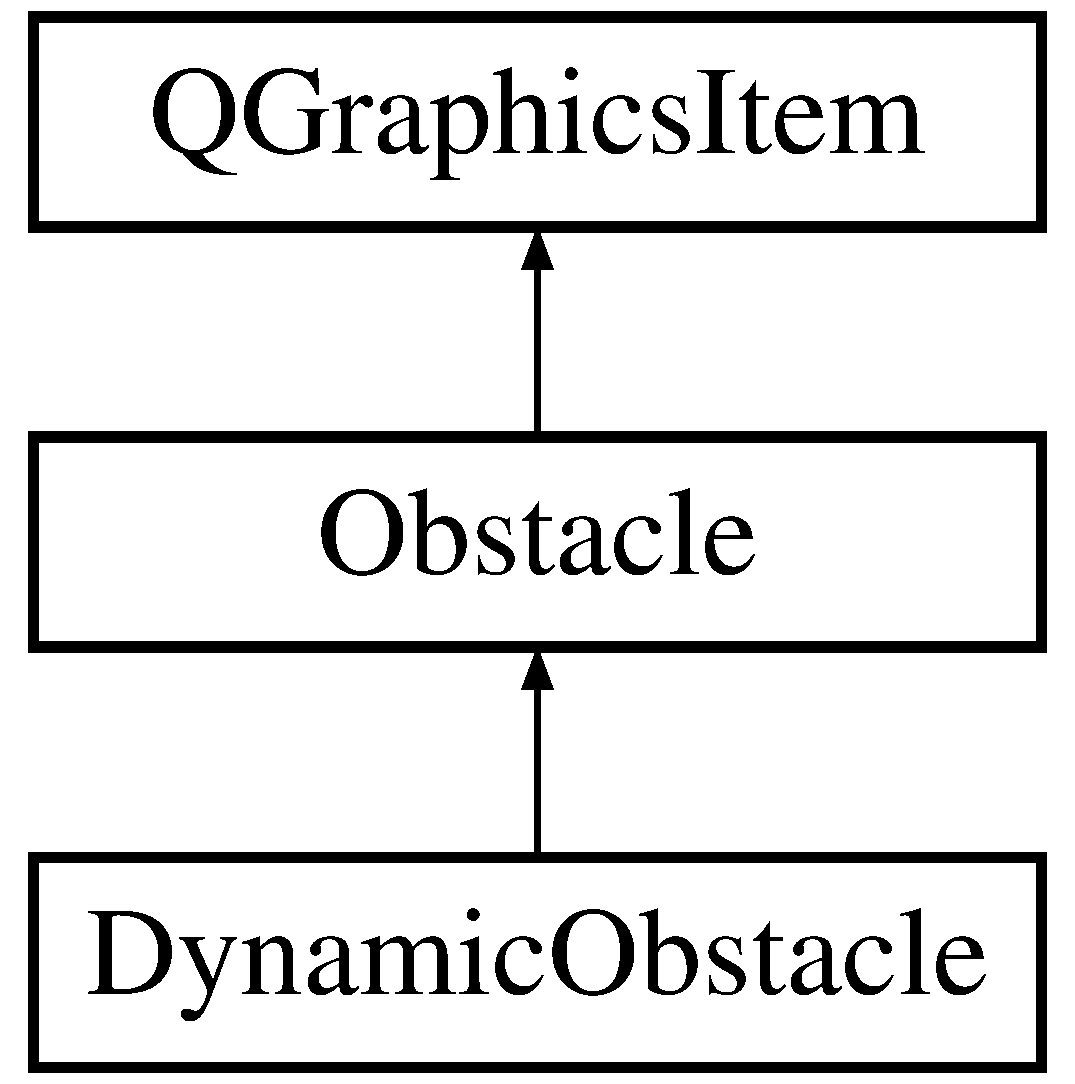
\includegraphics[height=3.000000cm]{class_obstacle}
\end{center}
\end{figure}
\subsection*{Public Member Functions}
\begin{DoxyCompactItemize}
\item 
\mbox{\Hypertarget{class_obstacle_ad99ea2e5503c0f3ae2f23ff33005ea66}\label{class_obstacle_ad99ea2e5503c0f3ae2f23ff33005ea66}} 
void {\bfseries mouse\+Press\+Event} (Q\+Graphics\+Scene\+Mouse\+Event $\ast$event)
\item 
\mbox{\Hypertarget{class_obstacle_aee96980c04e985efb24934541fba293e}\label{class_obstacle_aee96980c04e985efb24934541fba293e}} 
void {\bfseries mouse\+Release\+Event} (Q\+Graphics\+Scene\+Mouse\+Event $\ast$event)
\item 
\mbox{\Hypertarget{class_obstacle_a9bf186d9151a4973369a5aef75a42e61}\label{class_obstacle_a9bf186d9151a4973369a5aef75a42e61}} 
void {\bfseries mouse\+Move\+Event} (Q\+Graphics\+Scene\+Mouse\+Event $\ast$event)
\item 
double \mbox{\hyperlink{class_obstacle_a2bf33211e30b7dd9292ff23f76a7d008}{getwidth}} ()
\item 
double \mbox{\hyperlink{class_obstacle_afe853d8607d0794e44d3507c47ad5761}{getlength}} ()
\item 
\mbox{\Hypertarget{class_obstacle_a340e003df47196b278dc1b3cbf66145d}\label{class_obstacle_a340e003df47196b278dc1b3cbf66145d}} 
virtual double {\bfseries get\+Speed} ()
\item 
\mbox{\Hypertarget{class_obstacle_a7025a08583ea3d3dc21778d2727fb89f}\label{class_obstacle_a7025a08583ea3d3dc21778d2727fb89f}} 
virtual void {\bfseries set\+Speed} (double s)
\item 
\mbox{\Hypertarget{class_obstacle_a4053849e0ecdb7b51be12e779c5dece1}\label{class_obstacle_a4053849e0ecdb7b51be12e779c5dece1}} 
bool {\bfseries is\+Clicked} ()
\item 
\mbox{\Hypertarget{class_obstacle_a7c0383da429b66fd9f7c28af4bb9e287}\label{class_obstacle_a7c0383da429b66fd9f7c28af4bb9e287}} 
void {\bfseries set\+Clicked} (bool c)
\item 
\mbox{\Hypertarget{class_obstacle_a038612ebb2bf5457eb1b447849a6a9b0}\label{class_obstacle_a038612ebb2bf5457eb1b447849a6a9b0}} 
void {\bfseries update\+Position} ()
\item 
void \mbox{\hyperlink{class_obstacle_a601d8574fb13298bf693f0e4a2a5982f}{set\+Position}} (double x, double y)
\item 
\mbox{\Hypertarget{class_obstacle_a99a30018b72dc2fdbe0641ebd9dbe7dc}\label{class_obstacle_a99a30018b72dc2fdbe0641ebd9dbe7dc}} 
virtual double {\bfseries calculate\+Rotation} ()
\item 
virtual Q\+RectF \mbox{\hyperlink{class_obstacle_a6f02b341e339ea27c3391a44c787b5f2}{bounding\+Rect}} () const
\item 
virtual void \mbox{\hyperlink{class_obstacle_a42945fd08ee06a3bc33199f4f2ca37c1}{paint}} (Q\+Painter $\ast$painter, const Q\+Style\+Option\+Graphics\+Item $\ast$option, Q\+Widget $\ast$widget)
\item 
virtual Q\+String \mbox{\hyperlink{class_obstacle_a14ba5e7996c9e0a0bd3afc3bea5771ea}{get\+Type}} ()
\item 
\mbox{\Hypertarget{class_obstacle_afccb1406e9f18b60f51da28213592379}\label{class_obstacle_afccb1406e9f18b60f51da28213592379}} 
virtual Q\+PointF {\bfseries get\+Starting\+Point} ()
\item 
\mbox{\Hypertarget{class_obstacle_a7b164b4542c63039e2a33af1fe571457}\label{class_obstacle_a7b164b4542c63039e2a33af1fe571457}} 
virtual Q\+PointF {\bfseries get\+Ending\+Point} ()
\item 
\mbox{\hyperlink{class_obstacle_a8f734072321fa06a7b7dae2d5f50f352}{Obstacle}} ()
\item 
\mbox{\hyperlink{class_obstacle_ab31bcc85e9865eb103d86196c640cbe5}{Obstacle}} (double x, double y, double width, double length)
\item 
Q\+PointF $\ast$ \mbox{\hyperlink{class_obstacle_acc23c6ded38190d10b50e6190a85744e}{get\+Position}} ()
\end{DoxyCompactItemize}
\subsection*{Protected Member Functions}
\begin{DoxyCompactItemize}
\item 
virtual void \mbox{\hyperlink{class_obstacle_ac3bcd488b16a8d8cf99875c6d0172e15}{advance}} (int phase)
\end{DoxyCompactItemize}
\subsection*{Protected Attributes}
\begin{DoxyCompactItemize}
\item 
\mbox{\Hypertarget{class_obstacle_a585c9f0982084573c2e1172076aac502}\label{class_obstacle_a585c9f0982084573c2e1172076aac502}} 
Q\+PointF $\ast$ {\bfseries position}
\item 
\mbox{\Hypertarget{class_obstacle_aea38cecf56d04b14398c07388c6cdc5d}\label{class_obstacle_aea38cecf56d04b14398c07388c6cdc5d}} 
double {\bfseries width}
\item 
\mbox{\Hypertarget{class_obstacle_a71008c9d9ddaa8faa92e3ec1973fc572}\label{class_obstacle_a71008c9d9ddaa8faa92e3ec1973fc572}} 
double {\bfseries length}
\item 
\mbox{\Hypertarget{class_obstacle_ae712955c5f72f3ac00e460702950130c}\label{class_obstacle_ae712955c5f72f3ac00e460702950130c}} 
bool {\bfseries clicked}
\end{DoxyCompactItemize}


\subsection{Detailed Description}
Klasse für statische Hindernisse 

\subsection{Constructor \& Destructor Documentation}
\mbox{\Hypertarget{class_obstacle_a8f734072321fa06a7b7dae2d5f50f352}\label{class_obstacle_a8f734072321fa06a7b7dae2d5f50f352}} 
\index{Obstacle@{Obstacle}!Obstacle@{Obstacle}}
\index{Obstacle@{Obstacle}!Obstacle@{Obstacle}}
\subsubsection{\texorpdfstring{Obstacle()}{Obstacle()}\hspace{0.1cm}{\footnotesize\ttfamily [1/2]}}
{\footnotesize\ttfamily Obstacle\+::\+Obstacle (\begin{DoxyParamCaption}{ }\end{DoxyParamCaption})}

Erstellt ein neues \mbox{\hyperlink{class_obstacle}{Obstacle}} ohne Größe und Position auf der \mbox{\hyperlink{class_map}{Map}} \mbox{\Hypertarget{class_obstacle_ab31bcc85e9865eb103d86196c640cbe5}\label{class_obstacle_ab31bcc85e9865eb103d86196c640cbe5}} 
\index{Obstacle@{Obstacle}!Obstacle@{Obstacle}}
\index{Obstacle@{Obstacle}!Obstacle@{Obstacle}}
\subsubsection{\texorpdfstring{Obstacle()}{Obstacle()}\hspace{0.1cm}{\footnotesize\ttfamily [2/2]}}
{\footnotesize\ttfamily Obstacle\+::\+Obstacle (\begin{DoxyParamCaption}\item[{double}]{x,  }\item[{double}]{y,  }\item[{double}]{width,  }\item[{double}]{length }\end{DoxyParamCaption})}

Erstellt ein neues \mbox{\hyperlink{class_obstacle}{Obstacle}} 
\begin{DoxyParams}{Parameters}
{\em x} & x-\/\+Koordinate des \mbox{\hyperlink{class_obstacle}{Obstacle}} \\
\hline
{\em y} & y-\/\+Koordinate des \mbox{\hyperlink{class_obstacle}{Obstacle}} \\
\hline
{\em width} & Breite des \mbox{\hyperlink{class_obstacle}{Obstacle}} \\
\hline
{\em length} & Höhe des \mbox{\hyperlink{class_obstacle}{Obstacle}} \\
\hline
\end{DoxyParams}


\subsection{Member Function Documentation}
\mbox{\Hypertarget{class_obstacle_ac3bcd488b16a8d8cf99875c6d0172e15}\label{class_obstacle_ac3bcd488b16a8d8cf99875c6d0172e15}} 
\index{Obstacle@{Obstacle}!advance@{advance}}
\index{advance@{advance}!Obstacle@{Obstacle}}
\subsubsection{\texorpdfstring{advance()}{advance()}}
{\footnotesize\ttfamily void Obstacle\+::advance (\begin{DoxyParamCaption}\item[{int}]{phase }\end{DoxyParamCaption})\hspace{0.3cm}{\ttfamily [protected]}, {\ttfamily [virtual]}}

Wählt ein \mbox{\hyperlink{class_obstacle}{Obstacle}} an, wenn es angeklickt wurde 

Reimplemented in \mbox{\hyperlink{class_dynamic_obstacle_a533d0927fbe09aa105c47e00b1cd045f}{Dynamic\+Obstacle}}.

\mbox{\Hypertarget{class_obstacle_a6f02b341e339ea27c3391a44c787b5f2}\label{class_obstacle_a6f02b341e339ea27c3391a44c787b5f2}} 
\index{Obstacle@{Obstacle}!bounding\+Rect@{bounding\+Rect}}
\index{bounding\+Rect@{bounding\+Rect}!Obstacle@{Obstacle}}
\subsubsection{\texorpdfstring{bounding\+Rect()}{boundingRect()}}
{\footnotesize\ttfamily Q\+RectF Obstacle\+::bounding\+Rect (\begin{DoxyParamCaption}{ }\end{DoxyParamCaption}) const\hspace{0.3cm}{\ttfamily [virtual]}}

Erstellt ein Begrenzungsrechteck für das \mbox{\hyperlink{class_obstacle}{Obstacle}}. Dieses wird sowohl zum zeichnen, als auch für weitere Interaktion benötigt \begin{DoxyReturn}{Returns}
Begrenzungsrechteck des \mbox{\hyperlink{class_obstacle}{Obstacle}} 
\end{DoxyReturn}


Reimplemented in \mbox{\hyperlink{class_dynamic_obstacle_ac1b0b15d722a45decc8b77fcde22efd0}{Dynamic\+Obstacle}}.

\mbox{\Hypertarget{class_obstacle_afe853d8607d0794e44d3507c47ad5761}\label{class_obstacle_afe853d8607d0794e44d3507c47ad5761}} 
\index{Obstacle@{Obstacle}!getlength@{getlength}}
\index{getlength@{getlength}!Obstacle@{Obstacle}}
\subsubsection{\texorpdfstring{getlength()}{getlength()}}
{\footnotesize\ttfamily double Obstacle\+::getlength (\begin{DoxyParamCaption}{ }\end{DoxyParamCaption})}

Gibt die Länge des \mbox{\hyperlink{class_obstacle}{Obstacle}} zurück \begin{DoxyReturn}{Returns}
Länge des \mbox{\hyperlink{class_obstacle}{Obstacle}} 
\end{DoxyReturn}
\mbox{\Hypertarget{class_obstacle_acc23c6ded38190d10b50e6190a85744e}\label{class_obstacle_acc23c6ded38190d10b50e6190a85744e}} 
\index{Obstacle@{Obstacle}!get\+Position@{get\+Position}}
\index{get\+Position@{get\+Position}!Obstacle@{Obstacle}}
\subsubsection{\texorpdfstring{get\+Position()}{getPosition()}}
{\footnotesize\ttfamily Q\+PointF $\ast$ Obstacle\+::get\+Position (\begin{DoxyParamCaption}{ }\end{DoxyParamCaption})}

Gibt die Position des \mbox{\hyperlink{class_obstacle}{Obstacle}} zurück \begin{DoxyReturn}{Returns}
Position des \mbox{\hyperlink{class_obstacle}{Obstacle}} 
\end{DoxyReturn}
\mbox{\Hypertarget{class_obstacle_a14ba5e7996c9e0a0bd3afc3bea5771ea}\label{class_obstacle_a14ba5e7996c9e0a0bd3afc3bea5771ea}} 
\index{Obstacle@{Obstacle}!get\+Type@{get\+Type}}
\index{get\+Type@{get\+Type}!Obstacle@{Obstacle}}
\subsubsection{\texorpdfstring{get\+Type()}{getType()}}
{\footnotesize\ttfamily Q\+String Obstacle\+::get\+Type (\begin{DoxyParamCaption}{ }\end{DoxyParamCaption})\hspace{0.3cm}{\ttfamily [virtual]}}

Gibt den Typ des \mbox{\hyperlink{class_obstacle}{Obstacle}} zurück \begin{DoxyReturn}{Returns}
Typ des \mbox{\hyperlink{class_obstacle}{Obstacle}} 
\end{DoxyReturn}


Reimplemented in \mbox{\hyperlink{class_dynamic_obstacle_ac52c38ef60b99a7a29f89b6eb23df460}{Dynamic\+Obstacle}}.

\mbox{\Hypertarget{class_obstacle_a2bf33211e30b7dd9292ff23f76a7d008}\label{class_obstacle_a2bf33211e30b7dd9292ff23f76a7d008}} 
\index{Obstacle@{Obstacle}!getwidth@{getwidth}}
\index{getwidth@{getwidth}!Obstacle@{Obstacle}}
\subsubsection{\texorpdfstring{getwidth()}{getwidth()}}
{\footnotesize\ttfamily double Obstacle\+::getwidth (\begin{DoxyParamCaption}{ }\end{DoxyParamCaption})}

Gibt die Breite des \mbox{\hyperlink{class_obstacle}{Obstacle}} zurück \begin{DoxyReturn}{Returns}
Breite des \mbox{\hyperlink{class_obstacle}{Obstacle}} 
\end{DoxyReturn}
\mbox{\Hypertarget{class_obstacle_a42945fd08ee06a3bc33199f4f2ca37c1}\label{class_obstacle_a42945fd08ee06a3bc33199f4f2ca37c1}} 
\index{Obstacle@{Obstacle}!paint@{paint}}
\index{paint@{paint}!Obstacle@{Obstacle}}
\subsubsection{\texorpdfstring{paint()}{paint()}}
{\footnotesize\ttfamily void Obstacle\+::paint (\begin{DoxyParamCaption}\item[{Q\+Painter $\ast$}]{painter,  }\item[{const Q\+Style\+Option\+Graphics\+Item $\ast$}]{option,  }\item[{Q\+Widget $\ast$}]{widget }\end{DoxyParamCaption})\hspace{0.3cm}{\ttfamily [virtual]}}

Zeichnet das \mbox{\hyperlink{class_obstacle}{Obstacle}} 
\begin{DoxyParams}{Parameters}
{\em painter} & Painter der zum zeichnen benutzt wird \\
\hline
{\em option} & Optionen für das Zeichnen \\
\hline
{\em widget} & Widget in welches gezeichnet wird \\
\hline
\end{DoxyParams}


Reimplemented in \mbox{\hyperlink{class_dynamic_obstacle_a30c0753280f05f69a9da89bc9d9ce3f6}{Dynamic\+Obstacle}}.

\mbox{\Hypertarget{class_obstacle_a601d8574fb13298bf693f0e4a2a5982f}\label{class_obstacle_a601d8574fb13298bf693f0e4a2a5982f}} 
\index{Obstacle@{Obstacle}!set\+Position@{set\+Position}}
\index{set\+Position@{set\+Position}!Obstacle@{Obstacle}}
\subsubsection{\texorpdfstring{set\+Position()}{setPosition()}}
{\footnotesize\ttfamily void Obstacle\+::set\+Position (\begin{DoxyParamCaption}\item[{double}]{x,  }\item[{double}]{y }\end{DoxyParamCaption})}

Verändert die Position des \mbox{\hyperlink{class_obstacle}{Obstacle}} 
\begin{DoxyParams}{Parameters}
{\em x} & neue x-\/\+Koordinate des \mbox{\hyperlink{class_obstacle}{Obstacle}} \\
\hline
{\em y} & neue y-\/\+Koordinate des \mbox{\hyperlink{class_obstacle}{Obstacle}} \\
\hline
\end{DoxyParams}


The documentation for this class was generated from the following files\+:\begin{DoxyCompactItemize}
\item 
D\+:/swt1718-\/editor/bin/source/obstacle.\+h\item 
D\+:/swt1718-\/editor/bin/source/obstacle.\+cpp\end{DoxyCompactItemize}

\hypertarget{class_point}{}\section{Point Class Reference}
\label{class_point}\index{Point@{Point}}


{\ttfamily \#include $<$point.\+h$>$}

\subsection*{Public Member Functions}
\begin{DoxyCompactItemize}
\item 
\mbox{\hyperlink{class_point_ad92f2337b839a94ce97dcdb439b4325a}{Point}} ()
\item 
\mbox{\hyperlink{class_point_ac48df7076af6d62f06c83dec7210af6f}{Point}} (double nx, double ny)
\item 
void \mbox{\hyperlink{class_point_a62436e2678bfd0a4be0e2729c9d60380}{setX}} (double nx)
\item 
void \mbox{\hyperlink{class_point_a3611975b72fc2279dc91653237bd3cd5}{setY}} (double ny)
\item 
double \mbox{\hyperlink{class_point_a8de35a6098cdd7267b4167776da83da6}{getX}} ()
\item 
double \mbox{\hyperlink{class_point_aa278c8bcb8aeb4101023a4baf473b547}{getY}} ()
\item 
\mbox{\hyperlink{class_point}{Point}} \mbox{\hyperlink{class_point_a4fabca990b4e246773cada554b22ff5d}{operator=}} (\mbox{\hyperlink{class_point}{Point}} $\ast$np)
\end{DoxyCompactItemize}


\subsection{Detailed Description}
Definiert einen Punkt in der x-\/y-\/\+Ebene 

\subsection{Constructor \& Destructor Documentation}
\mbox{\Hypertarget{class_point_ad92f2337b839a94ce97dcdb439b4325a}\label{class_point_ad92f2337b839a94ce97dcdb439b4325a}} 
\index{Point@{Point}!Point@{Point}}
\index{Point@{Point}!Point@{Point}}
\subsubsection{\texorpdfstring{Point()}{Point()}\hspace{0.1cm}{\footnotesize\ttfamily [1/2]}}
{\footnotesize\ttfamily Point\+::\+Point (\begin{DoxyParamCaption}{ }\end{DoxyParamCaption})}

Erstellt einen neuen Punkt im Koordinatenursprung \mbox{\Hypertarget{class_point_ac48df7076af6d62f06c83dec7210af6f}\label{class_point_ac48df7076af6d62f06c83dec7210af6f}} 
\index{Point@{Point}!Point@{Point}}
\index{Point@{Point}!Point@{Point}}
\subsubsection{\texorpdfstring{Point()}{Point()}\hspace{0.1cm}{\footnotesize\ttfamily [2/2]}}
{\footnotesize\ttfamily Point\+::\+Point (\begin{DoxyParamCaption}\item[{double}]{nx,  }\item[{double}]{ny }\end{DoxyParamCaption})}

Erstellt einen Punkt 
\begin{DoxyParams}{Parameters}
{\em nx} & x-\/\+Koordinate des Punktes \\
\hline
{\em ny} & y-\/\+Koordinate des Punktes \\
\hline
\end{DoxyParams}
\begin{DoxyReturn}{Returns}
Punkt mit den Koordinaten (nx,ny) 
\end{DoxyReturn}


\subsection{Member Function Documentation}
\mbox{\Hypertarget{class_point_a8de35a6098cdd7267b4167776da83da6}\label{class_point_a8de35a6098cdd7267b4167776da83da6}} 
\index{Point@{Point}!getX@{getX}}
\index{getX@{getX}!Point@{Point}}
\subsubsection{\texorpdfstring{get\+X()}{getX()}}
{\footnotesize\ttfamily double Point\+::getX (\begin{DoxyParamCaption}{ }\end{DoxyParamCaption})}

Gibt die x-\/\+Koordinate des Punktes zurück \begin{DoxyReturn}{Returns}
x-\/\+Koordinate des Punktes 
\end{DoxyReturn}
\mbox{\Hypertarget{class_point_aa278c8bcb8aeb4101023a4baf473b547}\label{class_point_aa278c8bcb8aeb4101023a4baf473b547}} 
\index{Point@{Point}!getY@{getY}}
\index{getY@{getY}!Point@{Point}}
\subsubsection{\texorpdfstring{get\+Y()}{getY()}}
{\footnotesize\ttfamily double Point\+::getY (\begin{DoxyParamCaption}{ }\end{DoxyParamCaption})}

Gibt die y-\/\+Koordinate des Punktes zurück \begin{DoxyReturn}{Returns}
y-\/\+Koordinate des Punktes 
\end{DoxyReturn}
\mbox{\Hypertarget{class_point_a4fabca990b4e246773cada554b22ff5d}\label{class_point_a4fabca990b4e246773cada554b22ff5d}} 
\index{Point@{Point}!operator=@{operator=}}
\index{operator=@{operator=}!Point@{Point}}
\subsubsection{\texorpdfstring{operator=()}{operator=()}}
{\footnotesize\ttfamily \mbox{\hyperlink{class_point}{Point}} Point\+::operator= (\begin{DoxyParamCaption}\item[{\mbox{\hyperlink{class_point}{Point}} $\ast$}]{np }\end{DoxyParamCaption})}

Setzt einen Punkt auf einen anderen Punkt 
\begin{DoxyParams}{Parameters}
{\em np} & Punkt dessen Koordinaten übernommen werden sollen \\
\hline
\end{DoxyParams}
\begin{DoxyReturn}{Returns}
Punkt mit den Koordinaten vom Punkt np 
\end{DoxyReturn}
\mbox{\Hypertarget{class_point_a62436e2678bfd0a4be0e2729c9d60380}\label{class_point_a62436e2678bfd0a4be0e2729c9d60380}} 
\index{Point@{Point}!setX@{setX}}
\index{setX@{setX}!Point@{Point}}
\subsubsection{\texorpdfstring{set\+X()}{setX()}}
{\footnotesize\ttfamily void Point\+::setX (\begin{DoxyParamCaption}\item[{double}]{nx }\end{DoxyParamCaption})}

Verändert die x-\/\+Koordinate des Punktes 
\begin{DoxyParams}{Parameters}
{\em nx} & neue x-\/\+Koordinate des Punktes \\
\hline
\end{DoxyParams}
\mbox{\Hypertarget{class_point_a3611975b72fc2279dc91653237bd3cd5}\label{class_point_a3611975b72fc2279dc91653237bd3cd5}} 
\index{Point@{Point}!setY@{setY}}
\index{setY@{setY}!Point@{Point}}
\subsubsection{\texorpdfstring{set\+Y()}{setY()}}
{\footnotesize\ttfamily void Point\+::setY (\begin{DoxyParamCaption}\item[{double}]{ny }\end{DoxyParamCaption})}

Verändert die y-\/\+Koordinate des Punktes 
\begin{DoxyParams}{Parameters}
{\em ny} & neue y-\/\+Koordinate des Punktes \\
\hline
\end{DoxyParams}


The documentation for this class was generated from the following files\+:\begin{DoxyCompactItemize}
\item 
D\+:/swt1718-\/editor/bin/source/point.\+h\item 
D\+:/swt1718-\/editor/bin/source/point.\+cpp\end{DoxyCompactItemize}

\hypertarget{class_sensor}{}\section{Sensor Class Reference}
\label{class_sensor}\index{Sensor@{Sensor}}
Inheritance diagram for Sensor\+:\begin{figure}[H]
\begin{center}
\leavevmode
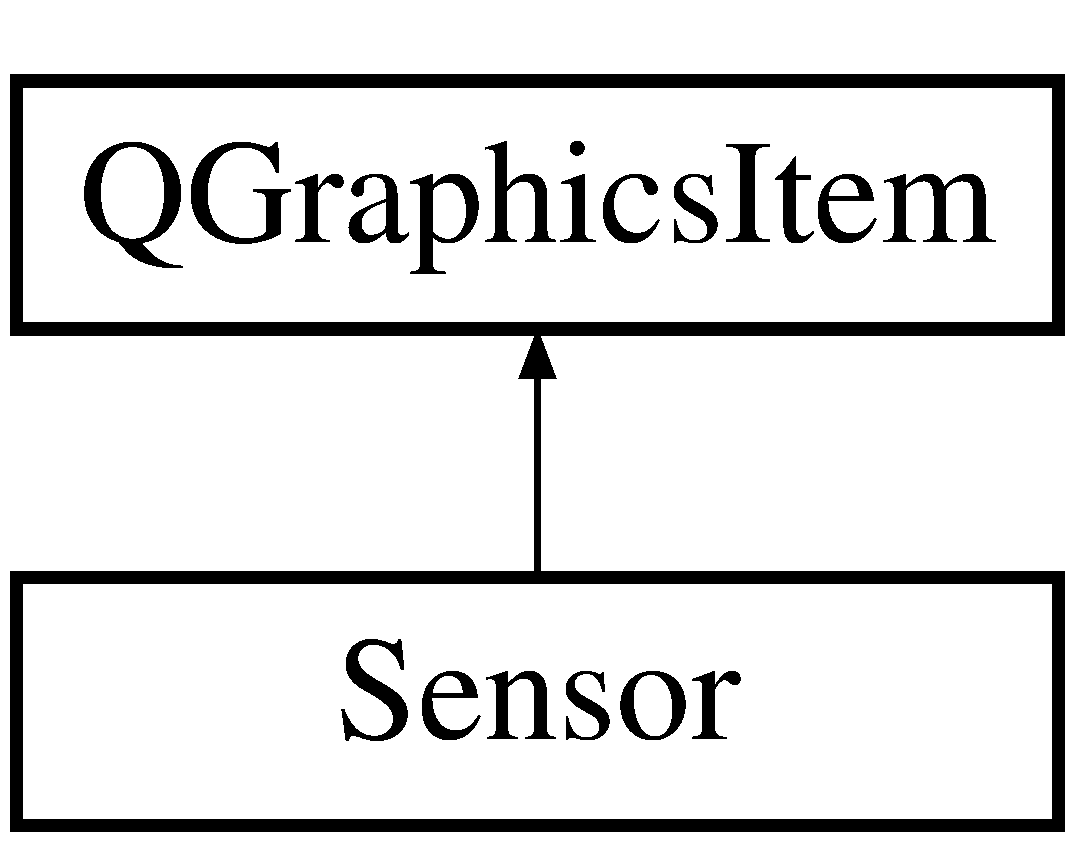
\includegraphics[height=2.000000cm]{class_sensor}
\end{center}
\end{figure}
\subsection*{Public Member Functions}
\begin{DoxyCompactItemize}
\item 
\mbox{\Hypertarget{class_sensor_a71e724fc8e79caa6b30532a51562113a}\label{class_sensor_a71e724fc8e79caa6b30532a51562113a}} 
{\bfseries Sensor} (int nangle, int nlength, Q\+PointF p)
\item 
\mbox{\Hypertarget{class_sensor_a50ae976cd9319902385aa762f4249ed7}\label{class_sensor_a50ae976cd9319902385aa762f4249ed7}} 
virtual Q\+RectF {\bfseries bounding\+Rect} () const
\item 
\mbox{\Hypertarget{class_sensor_a8f9855fbd3fa69c00c0065aa3d1bdc45}\label{class_sensor_a8f9855fbd3fa69c00c0065aa3d1bdc45}} 
virtual void {\bfseries paint} (Q\+Painter $\ast$painter, const Q\+Style\+Option\+Graphics\+Item $\ast$option, Q\+Widget $\ast$widget)
\item 
\mbox{\Hypertarget{class_sensor_ab8b342c87c06018a244c835876d9fe85}\label{class_sensor_ab8b342c87c06018a244c835876d9fe85}} 
int {\bfseries get\+Angle} ()
\item 
\mbox{\Hypertarget{class_sensor_a460531f1ab73104c15ad8975d961cdac}\label{class_sensor_a460531f1ab73104c15ad8975d961cdac}} 
int {\bfseries get\+Length} ()
\item 
\mbox{\Hypertarget{class_sensor_af1a08c6f7a5b84cf96bd2e0bbe5c25cf}\label{class_sensor_af1a08c6f7a5b84cf96bd2e0bbe5c25cf}} 
void {\bfseries set\+Color} (Q\+Color c)
\item 
\mbox{\Hypertarget{class_sensor_a623f89bd32e060295f338bf83c03ffaf}\label{class_sensor_a623f89bd32e060295f338bf83c03ffaf}} 
void {\bfseries set\+Length} (int nlength)
\item 
\mbox{\Hypertarget{class_sensor_a15e923daca628cd14d77c102e19ca523}\label{class_sensor_a15e923daca628cd14d77c102e19ca523}} 
void {\bfseries set\+Angle} (int nangle)
\item 
\mbox{\Hypertarget{class_sensor_a202df6c7c51ea7382cf3bcf07c7c2a0b}\label{class_sensor_a202df6c7c51ea7382cf3bcf07c7c2a0b}} 
void {\bfseries reset\+Rotation} ()
\end{DoxyCompactItemize}


The documentation for this class was generated from the following files\+:\begin{DoxyCompactItemize}
\item 
D\+:/swt1718-\/editor/bin/source/sensor.\+h\item 
D\+:/swt1718-\/editor/bin/source/sensor.\+cpp\end{DoxyCompactItemize}

\hypertarget{class_simulator}{}\section{Simulator Class Reference}
\label{class_simulator}\index{Simulator@{Simulator}}
Inheritance diagram for Simulator\+:\begin{figure}[H]
\begin{center}
\leavevmode
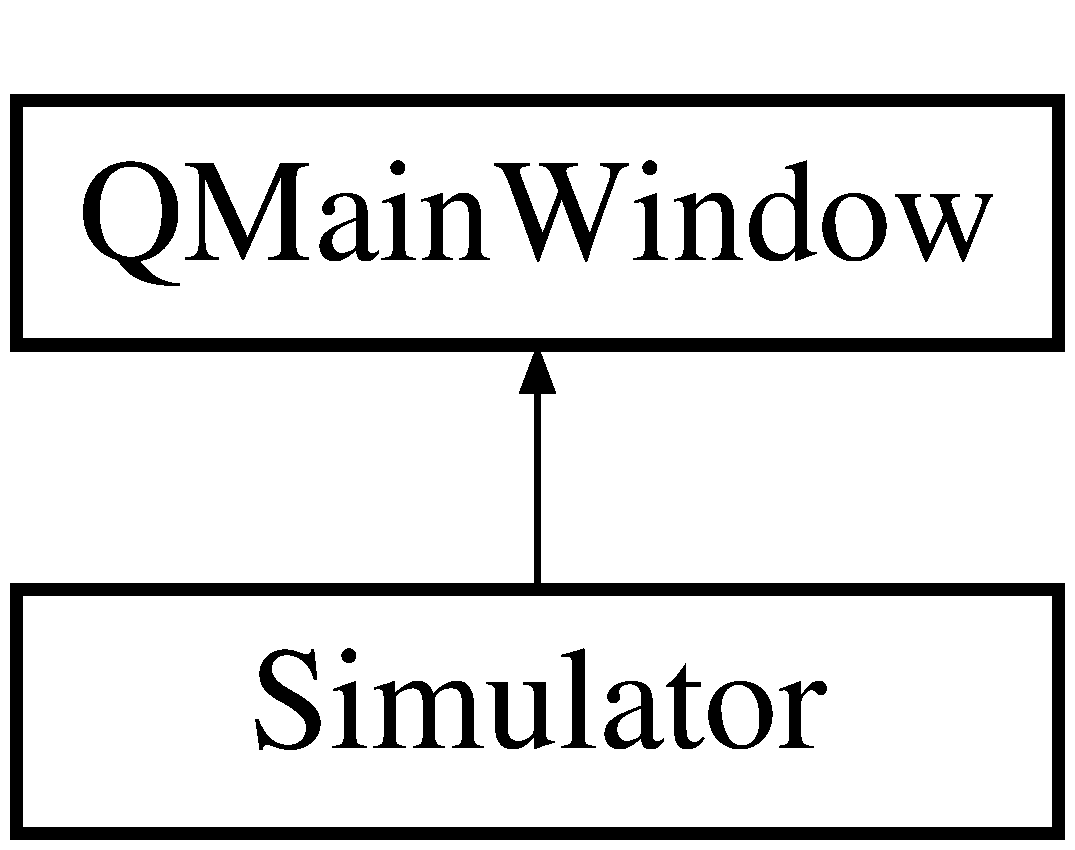
\includegraphics[height=2.000000cm]{class_simulator}
\end{center}
\end{figure}
\subsection*{Public Member Functions}
\begin{DoxyCompactItemize}
\item 
\mbox{\Hypertarget{class_simulator_abcf75e96d87dccb8eb87f6ded0c2d46f}\label{class_simulator_abcf75e96d87dccb8eb87f6ded0c2d46f}} 
{\bfseries Simulator} (Q\+Widget $\ast$parent=0)
\end{DoxyCompactItemize}


The documentation for this class was generated from the following files\+:\begin{DoxyCompactItemize}
\item 
D\+:/swt1718-\/editor/bin/source/simulator.\+h\item 
D\+:/swt1718-\/editor/bin/source/simulator.\+cpp\end{DoxyCompactItemize}

\hypertarget{class_simulator_c_m_d_l}{}\section{Simulator\+C\+M\+DL Class Reference}
\label{class_simulator_c_m_d_l}\index{Simulator\+C\+M\+DL@{Simulator\+C\+M\+DL}}
Inheritance diagram for Simulator\+C\+M\+DL\+:\begin{figure}[H]
\begin{center}
\leavevmode
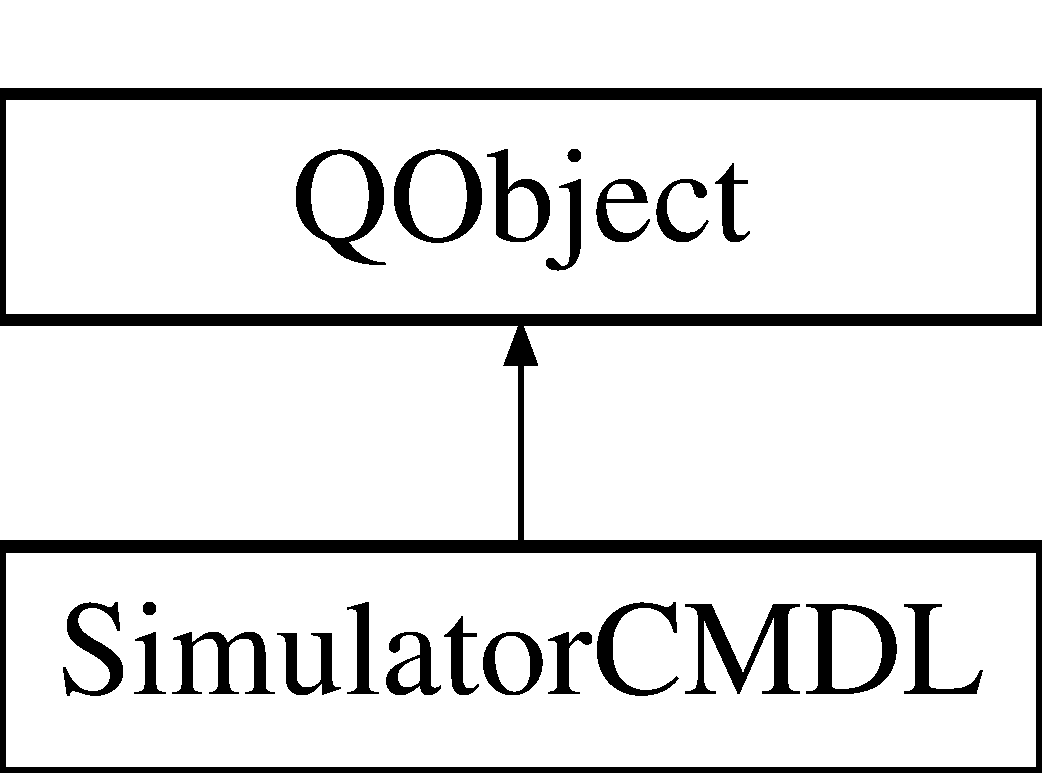
\includegraphics[height=2.000000cm]{class_simulator_c_m_d_l}
\end{center}
\end{figure}
\subsection*{Public Member Functions}
\begin{DoxyCompactItemize}
\item 
\mbox{\Hypertarget{class_simulator_c_m_d_l_a5059deaae21230537c97903334f2a241}\label{class_simulator_c_m_d_l_a5059deaae21230537c97903334f2a241}} 
{\bfseries Simulator\+C\+M\+DL} (\mbox{\hyperlink{class_map}{Map}} \&nm, Q\+Object $\ast$parent=nullptr)
\item 
\mbox{\Hypertarget{class_simulator_c_m_d_l_a60563f572993ad933245ed6e524776ca}\label{class_simulator_c_m_d_l_a60563f572993ad933245ed6e524776ca}} 
void {\bfseries start\+Simulation} ()
\item 
\mbox{\Hypertarget{class_simulator_c_m_d_l_ae84c6d1eef2acea326ebefef2655d099}\label{class_simulator_c_m_d_l_ae84c6d1eef2acea326ebefef2655d099}} 
void {\bfseries collision\+Detection} ()
\end{DoxyCompactItemize}


The documentation for this class was generated from the following files\+:\begin{DoxyCompactItemize}
\item 
D\+:/swt1718-\/editor/bin/source/simulatorcmdl.\+h\item 
D\+:/swt1718-\/editor/bin/source/simulatorcmdl.\+cpp\end{DoxyCompactItemize}

\hypertarget{class_simulator_window}{}\section{Simulator\+Window Class Reference}
\label{class_simulator_window}\index{Simulator\+Window@{Simulator\+Window}}
Inheritance diagram for Simulator\+Window\+:\begin{figure}[H]
\begin{center}
\leavevmode
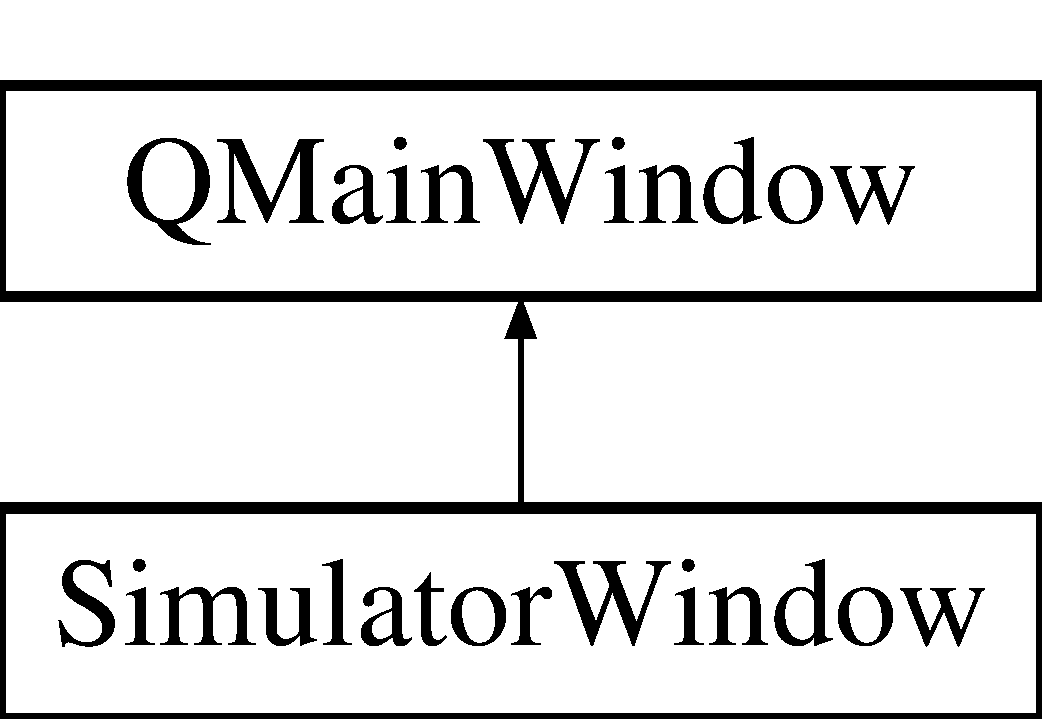
\includegraphics[height=2.000000cm]{class_simulator_window}
\end{center}
\end{figure}
\subsection*{Public Member Functions}
\begin{DoxyCompactItemize}
\item 
\mbox{\Hypertarget{class_simulator_window_adb262f9a95fb635130e46f007111634c}\label{class_simulator_window_adb262f9a95fb635130e46f007111634c}} 
{\bfseries Simulator\+Window} (const \mbox{\hyperlink{class_map}{Map}} \&nm, Q\+Widget $\ast$parent)
\item 
\mbox{\Hypertarget{class_simulator_window_a8e5b4f7ecb285477e56c1656e27a7113}\label{class_simulator_window_a8e5b4f7ecb285477e56c1656e27a7113}} 
void {\bfseries key\+Press\+Event} (Q\+Key\+Event $\ast$event)
\item 
\mbox{\Hypertarget{class_simulator_window_a3937f408fabc25c99089b98d45cf4807}\label{class_simulator_window_a3937f408fabc25c99089b98d45cf4807}} 
void {\bfseries key\+Release\+Event} (Q\+Key\+Event $\ast$event)
\item 
\mbox{\Hypertarget{class_simulator_window_a7551f243a88a306b947d34afd313e905}\label{class_simulator_window_a7551f243a88a306b947d34afd313e905}} 
void {\bfseries start\+Simulation} ()
\item 
\mbox{\Hypertarget{class_simulator_window_a98450d06554b6b88a9d9eb33244566cf}\label{class_simulator_window_a98450d06554b6b88a9d9eb33244566cf}} 
void {\bfseries physics} ()
\item 
\mbox{\Hypertarget{class_simulator_window_aae57e66151a2a6831f8a2d9aa39f6ea2}\label{class_simulator_window_aae57e66151a2a6831f8a2d9aa39f6ea2}} 
void {\bfseries save\+Net} ()
\item 
\mbox{\Hypertarget{class_simulator_window_af0e5cac29c16154c853b1bfe9bf1c46e}\label{class_simulator_window_af0e5cac29c16154c853b1bfe9bf1c46e}} 
void {\bfseries load\+Net} ()
\item 
\mbox{\Hypertarget{class_simulator_window_aa239fb1f5683451a7ebaa6e2a3c76c34}\label{class_simulator_window_aa239fb1f5683451a7ebaa6e2a3c76c34}} 
std\+::vector$<$ unsigned $>$ {\bfseries create\+Topology} ()
\item 
\mbox{\Hypertarget{class_simulator_window_ac9dc692851c4165653f4455f4c162676}\label{class_simulator_window_ac9dc692851c4165653f4455f4c162676}} 
void {\bfseries create\+Neural\+Net} (std\+::vector$<$ unsigned $>$ top)
\end{DoxyCompactItemize}


The documentation for this class was generated from the following files\+:\begin{DoxyCompactItemize}
\item 
D\+:/swt1718-\/editor/bin/source/simulatorwindow.\+h\item 
D\+:/swt1718-\/editor/bin/source/simulatorwindow.\+cpp\end{DoxyCompactItemize}

\hypertarget{class_smart_vehicle}{}\section{Smart\+Vehicle Class Reference}
\label{class_smart_vehicle}\index{Smart\+Vehicle@{Smart\+Vehicle}}
Inheritance diagram for Smart\+Vehicle\+:\begin{figure}[H]
\begin{center}
\leavevmode
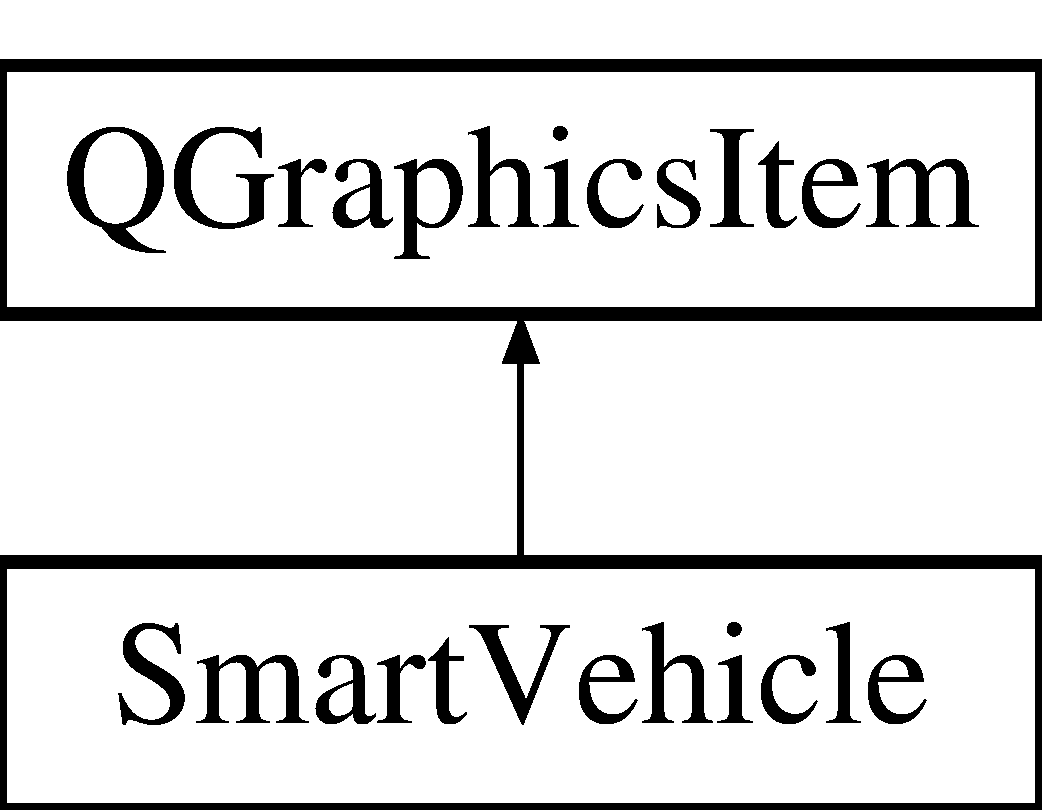
\includegraphics[height=2.000000cm]{class_smart_vehicle}
\end{center}
\end{figure}
\subsection*{Public Member Functions}
\begin{DoxyCompactItemize}
\item 
\mbox{\Hypertarget{class_smart_vehicle_a860c279d1237b674cb97dbf8fa0c0caa}\label{class_smart_vehicle_a860c279d1237b674cb97dbf8fa0c0caa}} 
{\bfseries Smart\+Vehicle} (int nangle, double nspeed, int nrotation\+Speed, int x, int y)
\item 
\mbox{\Hypertarget{class_smart_vehicle_afeaf1fc079e565e04cc54aeaca37f009}\label{class_smart_vehicle_afeaf1fc079e565e04cc54aeaca37f009}} 
virtual Q\+RectF {\bfseries bounding\+Rect} () const
\item 
\mbox{\Hypertarget{class_smart_vehicle_af241f76f0a49fbe6f4bf6754765c0165}\label{class_smart_vehicle_af241f76f0a49fbe6f4bf6754765c0165}} 
virtual void {\bfseries paint} (Q\+Painter $\ast$painter, const Q\+Style\+Option\+Graphics\+Item $\ast$option, Q\+Widget $\ast$widget)
\item 
\mbox{\Hypertarget{class_smart_vehicle_aa2c268069ba993619c389356ff37ee81}\label{class_smart_vehicle_aa2c268069ba993619c389356ff37ee81}} 
\mbox{\hyperlink{class_sensor}{Sensor}} $\ast$ {\bfseries get\+Sensor} (int i)
\item 
\mbox{\Hypertarget{class_smart_vehicle_a179e209c01fe810fa0ddc80e9bd43f4d}\label{class_smart_vehicle_a179e209c01fe810fa0ddc80e9bd43f4d}} 
void {\bfseries left} ()
\item 
\mbox{\Hypertarget{class_smart_vehicle_afae0834eded3c64f6c86ba65e40d3cb7}\label{class_smart_vehicle_afae0834eded3c64f6c86ba65e40d3cb7}} 
void {\bfseries right} ()
\item 
\mbox{\Hypertarget{class_smart_vehicle_a07331c47cda1eac0b0e361d928528301}\label{class_smart_vehicle_a07331c47cda1eac0b0e361d928528301}} 
void {\bfseries set\+Color} (Q\+Color c)
\item 
\mbox{\Hypertarget{class_smart_vehicle_a34651fae46b40981c089396b534d049a}\label{class_smart_vehicle_a34651fae46b40981c089396b534d049a}} 
void {\bfseries set\+Speed} (double nspeed)
\item 
\mbox{\Hypertarget{class_smart_vehicle_a87ffff9d67d4ca184761679be391a420}\label{class_smart_vehicle_a87ffff9d67d4ca184761679be391a420}} 
void {\bfseries set\+Angle} (int nangle)
\item 
\mbox{\Hypertarget{class_smart_vehicle_a46108297333e9498b7ee4a9fedcedcd1}\label{class_smart_vehicle_a46108297333e9498b7ee4a9fedcedcd1}} 
void {\bfseries reset\+Sensors} ()
\item 
\mbox{\Hypertarget{class_smart_vehicle_ad10b34691deb1f4548d65d947e80b321}\label{class_smart_vehicle_ad10b34691deb1f4548d65d947e80b321}} 
double {\bfseries get\+Speed} ()
\item 
\mbox{\Hypertarget{class_smart_vehicle_aa69d1e80908e922a5559af3e1ba122fc}\label{class_smart_vehicle_aa69d1e80908e922a5559af3e1ba122fc}} 
int {\bfseries get\+Number\+Of\+Sensors} ()
\end{DoxyCompactItemize}
\subsection*{Protected Member Functions}
\begin{DoxyCompactItemize}
\item 
\mbox{\Hypertarget{class_smart_vehicle_a4f210dfd0c2cd4d6a009bea627b978df}\label{class_smart_vehicle_a4f210dfd0c2cd4d6a009bea627b978df}} 
void {\bfseries advance} (int phase)
\end{DoxyCompactItemize}


The documentation for this class was generated from the following files\+:\begin{DoxyCompactItemize}
\item 
D\+:/swt1718-\/editor/bin/source/smartvehicle.\+h\item 
D\+:/swt1718-\/editor/bin/source/smartvehicle.\+cpp\end{DoxyCompactItemize}

\hypertarget{class_startingtile}{}\section{Startingtile Class Reference}
\label{class_startingtile}\index{Startingtile@{Startingtile}}
Inheritance diagram for Startingtile\+:\begin{figure}[H]
\begin{center}
\leavevmode
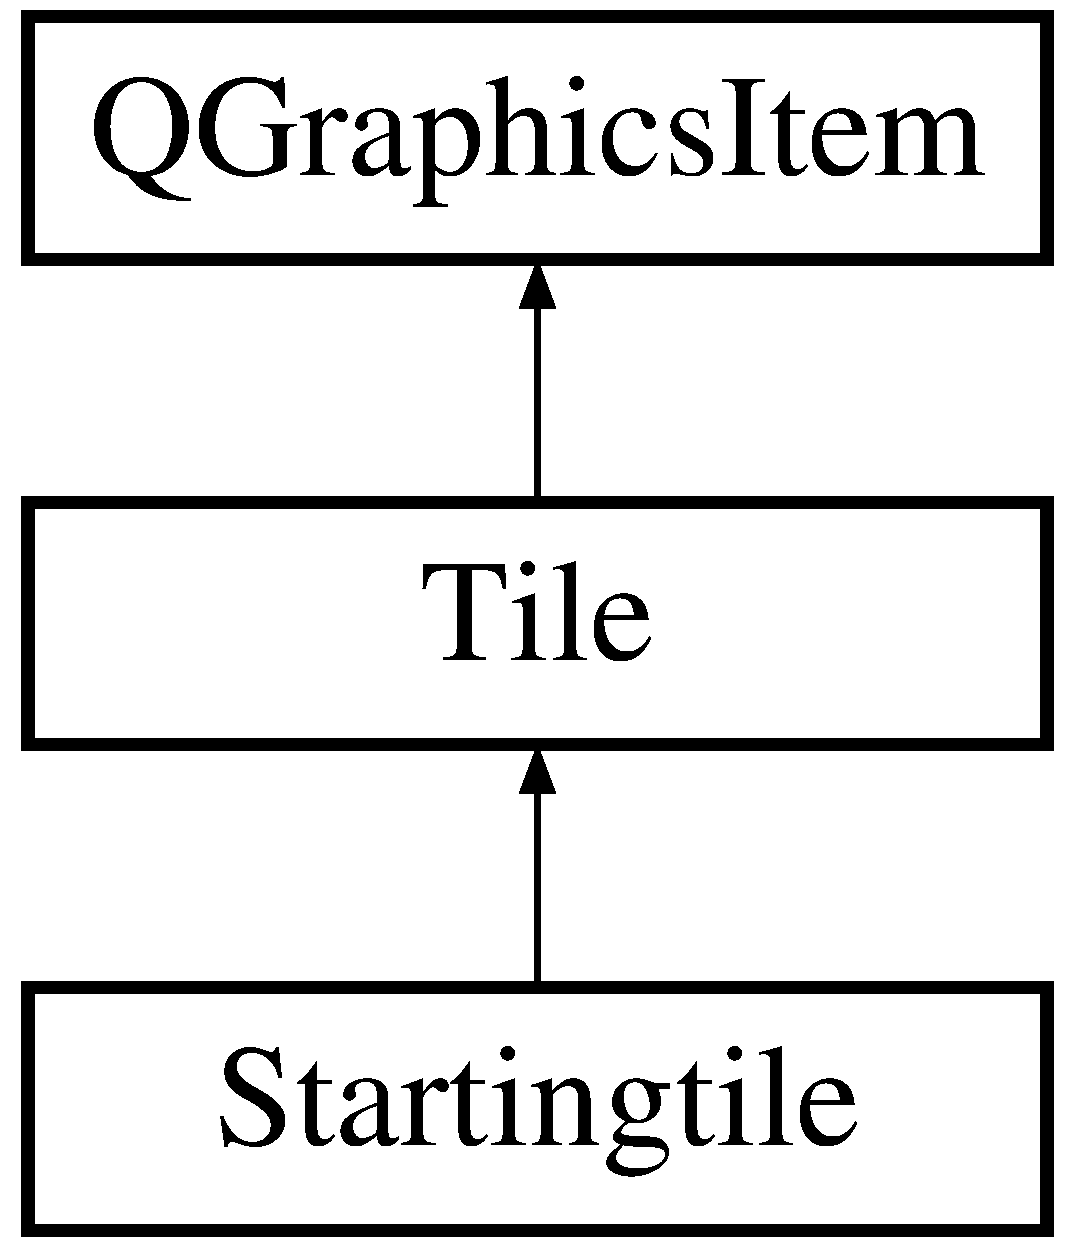
\includegraphics[height=3.000000cm]{class_startingtile}
\end{center}
\end{figure}
\subsection*{Public Member Functions}
\begin{DoxyCompactItemize}
\item 
virtual Q\+RectF \mbox{\hyperlink{class_startingtile_adfdbbb769775bf4a71f42795a3ca5cc7}{bounding\+Rect}} () const
\item 
virtual void \mbox{\hyperlink{class_startingtile_a125d0c3c2c814103a172c08180258d17}{paint}} (Q\+Painter $\ast$painter, const Q\+Style\+Option\+Graphics\+Item $\ast$option, Q\+Widget $\ast$widget)
\item 
virtual Q\+String \mbox{\hyperlink{class_startingtile_af9014bd47962800743b2057b520546d7}{get\+Type}} ()
\item 
void \mbox{\hyperlink{class_startingtile_aa2a399114844375bb6900b87f39ad946}{rotate}} ()
\end{DoxyCompactItemize}
\subsection*{Static Public Member Functions}
\begin{DoxyCompactItemize}
\item 
static \mbox{\hyperlink{class_startingtile}{Startingtile}} $\ast$ \mbox{\hyperlink{class_startingtile_a802644c93a230d81ba5a21c87866a411}{create\+Starting\+Tile}} (int nx, int ny, double nascent, int ndirection)
\end{DoxyCompactItemize}
\subsection*{Additional Inherited Members}


\subsection{Member Function Documentation}
\mbox{\Hypertarget{class_startingtile_adfdbbb769775bf4a71f42795a3ca5cc7}\label{class_startingtile_adfdbbb769775bf4a71f42795a3ca5cc7}} 
\index{Startingtile@{Startingtile}!bounding\+Rect@{bounding\+Rect}}
\index{bounding\+Rect@{bounding\+Rect}!Startingtile@{Startingtile}}
\subsubsection{\texorpdfstring{bounding\+Rect()}{boundingRect()}}
{\footnotesize\ttfamily Q\+RectF Startingtile\+::bounding\+Rect (\begin{DoxyParamCaption}{ }\end{DoxyParamCaption}) const\hspace{0.3cm}{\ttfamily [virtual]}}

Erstellt ein Begrenzungsrechteck für das \mbox{\hyperlink{class_tile}{Tile}},Dieses wird sowohl zum zeichnen, als auch für weitere Interaktion benötigt \mbox{\Hypertarget{class_startingtile_a802644c93a230d81ba5a21c87866a411}\label{class_startingtile_a802644c93a230d81ba5a21c87866a411}} 
\index{Startingtile@{Startingtile}!create\+Starting\+Tile@{create\+Starting\+Tile}}
\index{create\+Starting\+Tile@{create\+Starting\+Tile}!Startingtile@{Startingtile}}
\subsubsection{\texorpdfstring{create\+Starting\+Tile()}{createStartingTile()}}
{\footnotesize\ttfamily \mbox{\hyperlink{class_startingtile}{Startingtile}} $\ast$ Startingtile\+::create\+Starting\+Tile (\begin{DoxyParamCaption}\item[{int}]{nx,  }\item[{int}]{ny,  }\item[{double}]{nascent,  }\item[{int}]{ndireciton }\end{DoxyParamCaption})\hspace{0.3cm}{\ttfamily [static]}}

Prüft ob die \mbox{\hyperlink{class_map}{Map}} schon einen Startabschnitt hat, falls nicht, wird einer Erzeugt \begin{DoxyReturn}{Returns}
Pointer der auf den Startabschnitt zeigt 
\end{DoxyReturn}
\mbox{\Hypertarget{class_startingtile_af9014bd47962800743b2057b520546d7}\label{class_startingtile_af9014bd47962800743b2057b520546d7}} 
\index{Startingtile@{Startingtile}!get\+Type@{get\+Type}}
\index{get\+Type@{get\+Type}!Startingtile@{Startingtile}}
\subsubsection{\texorpdfstring{get\+Type()}{getType()}}
{\footnotesize\ttfamily Q\+String Startingtile\+::get\+Type (\begin{DoxyParamCaption}{ }\end{DoxyParamCaption})\hspace{0.3cm}{\ttfamily [virtual]}}

Gibt den Typen des \mbox{\hyperlink{class_tile}{Tile}} zurück \begin{DoxyReturn}{Returns}
Typ des \mbox{\hyperlink{class_tile}{Tile}} 
\end{DoxyReturn}


Reimplemented from \mbox{\hyperlink{class_tile_ad1dbea94d96060491a2dc4c7b92b31ab}{Tile}}.

\mbox{\Hypertarget{class_startingtile_a125d0c3c2c814103a172c08180258d17}\label{class_startingtile_a125d0c3c2c814103a172c08180258d17}} 
\index{Startingtile@{Startingtile}!paint@{paint}}
\index{paint@{paint}!Startingtile@{Startingtile}}
\subsubsection{\texorpdfstring{paint()}{paint()}}
{\footnotesize\ttfamily void Startingtile\+::paint (\begin{DoxyParamCaption}\item[{Q\+Painter $\ast$}]{painter,  }\item[{const Q\+Style\+Option\+Graphics\+Item $\ast$}]{option,  }\item[{Q\+Widget $\ast$}]{widget }\end{DoxyParamCaption})\hspace{0.3cm}{\ttfamily [virtual]}}

Zeichnet das \mbox{\hyperlink{class_tile}{Tile}} 
\begin{DoxyParams}{Parameters}
{\em painter} & Painter der zum Zeichnen benutzt wird \\
\hline
{\em option} & Optionen für das Zeichnen \\
\hline
{\em widget} & Widget in welches gezeichnet wird \\
\hline
\end{DoxyParams}


Reimplemented from \mbox{\hyperlink{class_tile_ab0a7262b6fab842a7a467fcb2f7592eb}{Tile}}.

\mbox{\Hypertarget{class_startingtile_aa2a399114844375bb6900b87f39ad946}\label{class_startingtile_aa2a399114844375bb6900b87f39ad946}} 
\index{Startingtile@{Startingtile}!rotate@{rotate}}
\index{rotate@{rotate}!Startingtile@{Startingtile}}
\subsubsection{\texorpdfstring{rotate()}{rotate()}}
{\footnotesize\ttfamily void Startingtile\+::rotate (\begin{DoxyParamCaption}{ }\end{DoxyParamCaption})\hspace{0.3cm}{\ttfamily [virtual]}}

Rotiert das \mbox{\hyperlink{class_tile}{Tile}} 

Reimplemented from \mbox{\hyperlink{class_tile_a15c3d8260c8950d3461e3ba2849cd141}{Tile}}.



The documentation for this class was generated from the following files\+:\begin{DoxyCompactItemize}
\item 
D\+:/swt1718-\/editor/bin/source/startingtile.\+h\item 
D\+:/swt1718-\/editor/bin/source/startingtile.\+cpp\end{DoxyCompactItemize}

\hypertarget{classstraight}{}\section{straight Class Reference}
\label{classstraight}\index{straight@{straight}}


{\ttfamily \#include $<$straight.\+h$>$}

Inheritance diagram for straight\+:\begin{figure}[H]
\begin{center}
\leavevmode
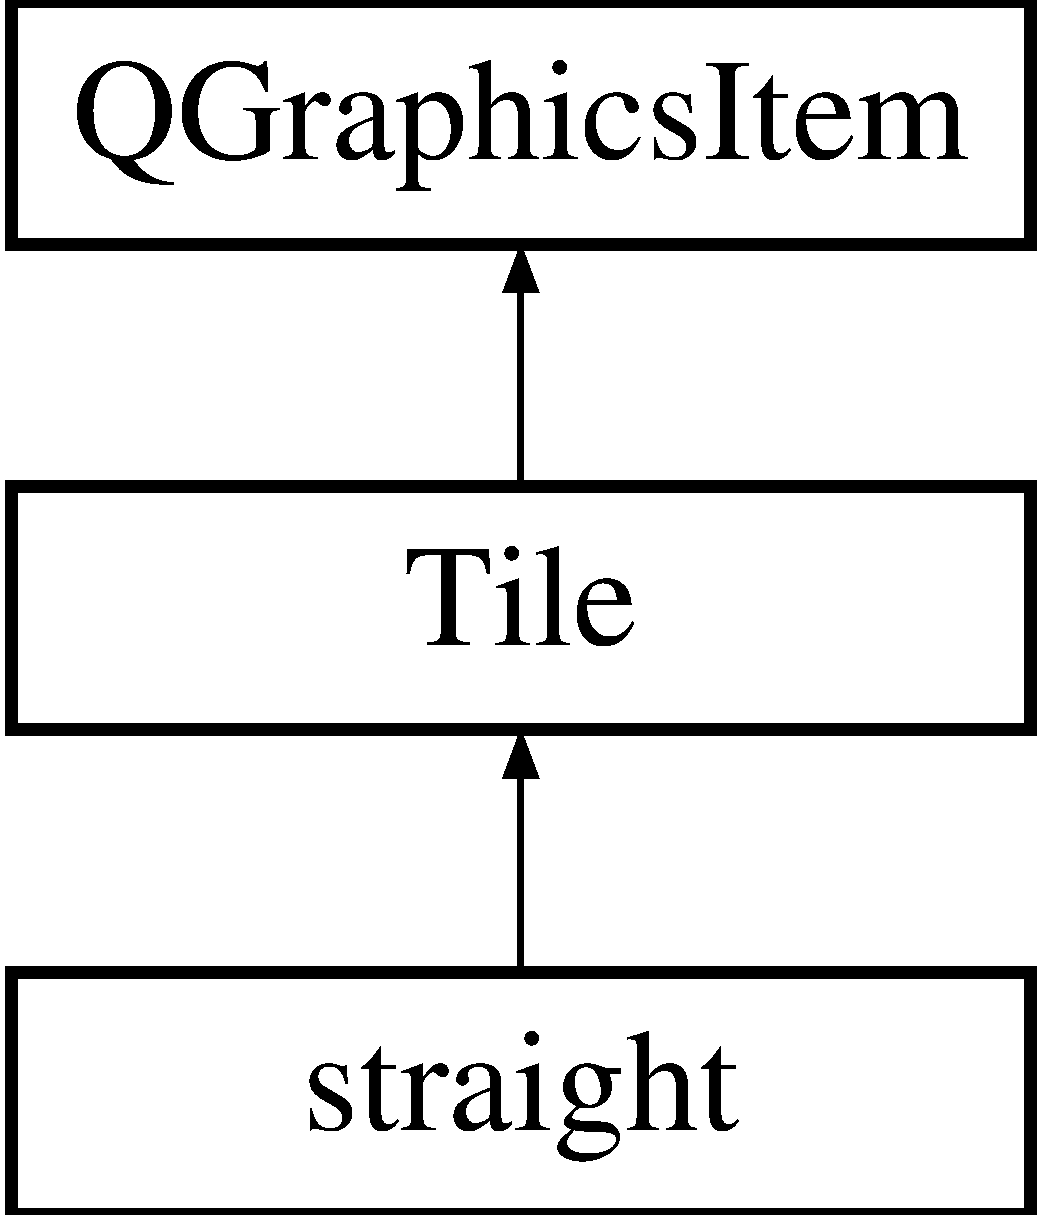
\includegraphics[height=3.000000cm]{classstraight}
\end{center}
\end{figure}
\subsection*{Public Member Functions}
\begin{DoxyCompactItemize}
\item 
\mbox{\hyperlink{classstraight_a0a1895927f40f1cc41debad219730cbe}{straight}} ()
\item 
\mbox{\hyperlink{classstraight_ac580066126df442eba57e77a00991659}{straight}} (double nx, double ny, double nascent, int ndirection)
\item 
Q\+RectF \mbox{\hyperlink{classstraight_a05add152ed81564fa3389b0a6f11cbc2}{bounding\+Rect}} () const
\item 
Q\+String \mbox{\hyperlink{classstraight_a50f5861f414dc03aa4e8947945abcd9e}{get\+Type}} ()
\item 
void \mbox{\hyperlink{classstraight_a324505038865a61ebe65542e29e7575a}{paint}} (Q\+Painter $\ast$painter, const Q\+Style\+Option\+Graphics\+Item $\ast$option, Q\+Widget $\ast$widget)
\item 
void \mbox{\hyperlink{classstraight_a2d60ee00c79e1c10f1bde4a46ea26bdb}{rotate}} ()
\end{DoxyCompactItemize}
\subsection*{Additional Inherited Members}


\subsection{Detailed Description}
Unterklasse von \mbox{\hyperlink{class_tile}{Tile}}, realisiert ein gerades Streckenstück 

\subsection{Constructor \& Destructor Documentation}
\mbox{\Hypertarget{classstraight_a0a1895927f40f1cc41debad219730cbe}\label{classstraight_a0a1895927f40f1cc41debad219730cbe}} 
\index{straight@{straight}!straight@{straight}}
\index{straight@{straight}!straight@{straight}}
\subsubsection{\texorpdfstring{straight()}{straight()}\hspace{0.1cm}{\footnotesize\ttfamily [1/2]}}
{\footnotesize\ttfamily straight\+::straight (\begin{DoxyParamCaption}{ }\end{DoxyParamCaption})}

Erstellt ein leeres gerades Streckenstück \mbox{\Hypertarget{classstraight_ac580066126df442eba57e77a00991659}\label{classstraight_ac580066126df442eba57e77a00991659}} 
\index{straight@{straight}!straight@{straight}}
\index{straight@{straight}!straight@{straight}}
\subsubsection{\texorpdfstring{straight()}{straight()}\hspace{0.1cm}{\footnotesize\ttfamily [2/2]}}
{\footnotesize\ttfamily straight\+::straight (\begin{DoxyParamCaption}\item[{double}]{nx,  }\item[{double}]{ny,  }\item[{double}]{nascent,  }\item[{int}]{ndirection }\end{DoxyParamCaption})}

Erstellt ein gerades Streckenstück 
\begin{DoxyParams}{Parameters}
{\em x} & x-\/\+Koordinate der Geraden \\
\hline
{\em y} & y-\/\+Koordinate der Geraden \\
\hline
{\em ascent} & Steigung der Geraden \\
\hline
\end{DoxyParams}


\subsection{Member Function Documentation}
\mbox{\Hypertarget{classstraight_a05add152ed81564fa3389b0a6f11cbc2}\label{classstraight_a05add152ed81564fa3389b0a6f11cbc2}} 
\index{straight@{straight}!bounding\+Rect@{bounding\+Rect}}
\index{bounding\+Rect@{bounding\+Rect}!straight@{straight}}
\subsubsection{\texorpdfstring{bounding\+Rect()}{boundingRect()}}
{\footnotesize\ttfamily Q\+RectF straight\+::bounding\+Rect (\begin{DoxyParamCaption}{ }\end{DoxyParamCaption}) const}

Erstellt ein Begrenzungsrechteck für das \mbox{\hyperlink{class_tile}{Tile}},Dieses wird sowohl zum zeichnen, als auch für weitere Interaktion benötigt \begin{DoxyReturn}{Returns}
Begrenzungsrechteck für das \mbox{\hyperlink{class_tile}{Tile}} 
\end{DoxyReturn}
\mbox{\Hypertarget{classstraight_a50f5861f414dc03aa4e8947945abcd9e}\label{classstraight_a50f5861f414dc03aa4e8947945abcd9e}} 
\index{straight@{straight}!get\+Type@{get\+Type}}
\index{get\+Type@{get\+Type}!straight@{straight}}
\subsubsection{\texorpdfstring{get\+Type()}{getType()}}
{\footnotesize\ttfamily Q\+String straight\+::get\+Type (\begin{DoxyParamCaption}{ }\end{DoxyParamCaption})\hspace{0.3cm}{\ttfamily [virtual]}}

Gibt den Typen des \mbox{\hyperlink{class_tile}{Tile}} zurück \begin{DoxyReturn}{Returns}
Typ des \mbox{\hyperlink{class_tile}{Tile}} 
\end{DoxyReturn}


Reimplemented from \mbox{\hyperlink{class_tile_ad1dbea94d96060491a2dc4c7b92b31ab}{Tile}}.

\mbox{\Hypertarget{classstraight_a324505038865a61ebe65542e29e7575a}\label{classstraight_a324505038865a61ebe65542e29e7575a}} 
\index{straight@{straight}!paint@{paint}}
\index{paint@{paint}!straight@{straight}}
\subsubsection{\texorpdfstring{paint()}{paint()}}
{\footnotesize\ttfamily void straight\+::paint (\begin{DoxyParamCaption}\item[{Q\+Painter $\ast$}]{painter,  }\item[{const Q\+Style\+Option\+Graphics\+Item $\ast$}]{option,  }\item[{Q\+Widget $\ast$}]{widget }\end{DoxyParamCaption})\hspace{0.3cm}{\ttfamily [virtual]}}

Zeichnet das \mbox{\hyperlink{class_tile}{Tile}} 
\begin{DoxyParams}{Parameters}
{\em painter} & Painter der zum Zeichnen benutzt wird \\
\hline
{\em option} & Optionen für das Zeichnen \\
\hline
{\em widget} & Widget in welches gezeichnet wird \\
\hline
\end{DoxyParams}


Reimplemented from \mbox{\hyperlink{class_tile_ab0a7262b6fab842a7a467fcb2f7592eb}{Tile}}.

\mbox{\Hypertarget{classstraight_a2d60ee00c79e1c10f1bde4a46ea26bdb}\label{classstraight_a2d60ee00c79e1c10f1bde4a46ea26bdb}} 
\index{straight@{straight}!rotate@{rotate}}
\index{rotate@{rotate}!straight@{straight}}
\subsubsection{\texorpdfstring{rotate()}{rotate()}}
{\footnotesize\ttfamily void straight\+::rotate (\begin{DoxyParamCaption}{ }\end{DoxyParamCaption})\hspace{0.3cm}{\ttfamily [virtual]}}

Rotiert das \mbox{\hyperlink{class_tile}{Tile}} um 90 Grad 

Reimplemented from \mbox{\hyperlink{class_tile_a15c3d8260c8950d3461e3ba2849cd141}{Tile}}.



The documentation for this class was generated from the following files\+:\begin{DoxyCompactItemize}
\item 
D\+:/swt1718-\/editor/bin/source/straight.\+h\item 
D\+:/swt1718-\/editor/bin/source/straight.\+cpp\end{DoxyCompactItemize}

\hypertarget{class_tile}{}\section{Tile Class Reference}
\label{class_tile}\index{Tile@{Tile}}


{\ttfamily \#include $<$tile.\+h$>$}

Inheritance diagram for Tile\+:\begin{figure}[H]
\begin{center}
\leavevmode
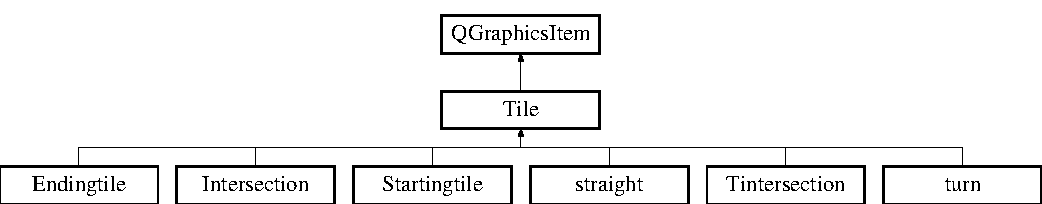
\includegraphics[height=2.718446cm]{class_tile}
\end{center}
\end{figure}
\subsection*{Public Member Functions}
\begin{DoxyCompactItemize}
\item 
\mbox{\hyperlink{class_tile_aeeb5593bb6b75aae2edfcccbc84ab378}{Tile}} ()
\item 
\mbox{\hyperlink{class_tile_a337c665729b9bc64eadcbf95623d5f89}{Tile}} (double x, double y, double ascent)
\item 
\mbox{\Hypertarget{class_tile_aaf4a05ad96a6889c3bb57c1cf08a329f}\label{class_tile_aaf4a05ad96a6889c3bb57c1cf08a329f}} 
bool {\bfseries is\+Clicked} ()
\item 
\mbox{\Hypertarget{class_tile_a533f76209d1ca3901b5898396332b70d}\label{class_tile_a533f76209d1ca3901b5898396332b70d}} 
void {\bfseries set\+Clicked} (bool c)
\item 
virtual Q\+RectF \mbox{\hyperlink{class_tile_a3ffc5a081e722e910f14053fcfb7b00f}{bounding\+Rect}} ()
\item 
virtual void \mbox{\hyperlink{class_tile_ab0a7262b6fab842a7a467fcb2f7592eb}{paint}} (Q\+Painter $\ast$painter, const Q\+Style\+Option\+Graphics\+Item $\ast$option, Q\+Widget $\ast$widget)
\item 
virtual Q\+String \mbox{\hyperlink{class_tile_ad1dbea94d96060491a2dc4c7b92b31ab}{get\+Type}} ()
\item 
double \mbox{\hyperlink{class_tile_a95d921c5d074181603edb6e2e8dd5389}{get\+Ascent}} ()
\item 
\mbox{\Hypertarget{class_tile_af8d69a6c278d2b8636aa23f88e47e2b0}\label{class_tile_af8d69a6c278d2b8636aa23f88e47e2b0}} 
int {\bfseries get\+Direction} ()
\item 
\mbox{\Hypertarget{class_tile_a0cd2136e09f22b4085769cd0a0b1389f}\label{class_tile_a0cd2136e09f22b4085769cd0a0b1389f}} 
void {\bfseries fit\+Into\+Grid} ()
\item 
\mbox{\Hypertarget{class_tile_af2f7be553412c7bc9f0b6dade741a17f}\label{class_tile_af2f7be553412c7bc9f0b6dade741a17f}} 
void {\bfseries fit\+Into\+Scene} ()
\item 
\mbox{\Hypertarget{class_tile_a44a8d80edfae3c7d4f47c61035984b3c}\label{class_tile_a44a8d80edfae3c7d4f47c61035984b3c}} 
void {\bfseries set\+Index} (int i)
\item 
void \mbox{\hyperlink{class_tile_a80d6dd0d052f39c01f8f261dfe53f08b}{set\+Position}} (double x, double y)
\item 
void \mbox{\hyperlink{class_tile_aa7621f21afe1b7405f56eef0c9c5a9fa}{set\+Ascent}} (double Ascent)
\item 
\mbox{\Hypertarget{class_tile_acafc1364871ec146744f443612cab725}\label{class_tile_acafc1364871ec146744f443612cab725}} 
void {\bfseries set\+Direction} (double ndirection)
\item 
\mbox{\Hypertarget{class_tile_ac43fd9fe874ef4ed6155b796a7cec9f8}\label{class_tile_ac43fd9fe874ef4ed6155b796a7cec9f8}} 
void {\bfseries set\+Path} (Q\+Painter\+Path p)
\item 
virtual void \mbox{\hyperlink{class_tile_a15c3d8260c8950d3461e3ba2849cd141}{rotate}} ()
\item 
void \mbox{\hyperlink{class_tile_af1674a1e05675b4771e1b603ca385d42}{mouse\+Double\+Click\+Event}} (Q\+Graphics\+Scene\+Mouse\+Event $\ast$event)
\item 
void \mbox{\hyperlink{class_tile_aecbd71c0de7fe3fd79bb1b8bbca4f265}{mouse\+Press\+Event}} (Q\+Graphics\+Scene\+Mouse\+Event $\ast$event)
\item 
\mbox{\Hypertarget{class_tile_a6be6db876fbc41e789dad725f954b705}\label{class_tile_a6be6db876fbc41e789dad725f954b705}} 
void {\bfseries mouse\+Release\+Event} (Q\+Graphics\+Scene\+Mouse\+Event $\ast$event)
\item 
Q\+Painter\+Path \mbox{\hyperlink{class_tile_a044239c0b2a4a24bf602ddba15ab0a01}{get\+Path}} ()
\item 
Q\+PointF $\ast$ \mbox{\hyperlink{class_tile_a8c2b6c2dfd8b381932454752558b1395}{get\+Position}} ()
\end{DoxyCompactItemize}
\subsection*{Protected Attributes}
\begin{DoxyCompactItemize}
\item 
\mbox{\Hypertarget{class_tile_ab9753327fa5861cc5c9b48c6ba632fca}\label{class_tile_ab9753327fa5861cc5c9b48c6ba632fca}} 
Q\+PointF $\ast$ {\bfseries position}
\item 
\mbox{\Hypertarget{class_tile_aeb69860ce29868082a9278d2f06b3400}\label{class_tile_aeb69860ce29868082a9278d2f06b3400}} 
double {\bfseries ascent}
\item 
\mbox{\Hypertarget{class_tile_ad3415390d272158aaf215f24e3df237d}\label{class_tile_ad3415390d272158aaf215f24e3df237d}} 
Q\+Painter\+Path {\bfseries path}
\item 
\mbox{\Hypertarget{class_tile_a148eb9ba30d682a2237ab8c82aacc8ef}\label{class_tile_a148eb9ba30d682a2237ab8c82aacc8ef}} 
int {\bfseries direction} = 0
\item 
\mbox{\Hypertarget{class_tile_af463934d32c7bc00ce055f5d9b43ad56}\label{class_tile_af463934d32c7bc00ce055f5d9b43ad56}} 
Q\+PointF {\bfseries top\+Left}
\item 
\mbox{\Hypertarget{class_tile_a72d12308d2f629ed6515906d6172cdf5}\label{class_tile_a72d12308d2f629ed6515906d6172cdf5}} 
Q\+PointF {\bfseries top\+Right}
\item 
\mbox{\Hypertarget{class_tile_ad5f0c9de4bf667069e3b15c76e342d3e}\label{class_tile_ad5f0c9de4bf667069e3b15c76e342d3e}} 
Q\+PointF {\bfseries bottom\+Right}
\item 
\mbox{\Hypertarget{class_tile_a8b0e49655a83f4ba963d60ed090691e6}\label{class_tile_a8b0e49655a83f4ba963d60ed090691e6}} 
Q\+PointF {\bfseries bottom\+Left}
\item 
\mbox{\Hypertarget{class_tile_aec5e69248a51b044658dd2a003e688e0}\label{class_tile_aec5e69248a51b044658dd2a003e688e0}} 
Q\+PointF {\bfseries top\+Center}
\item 
\mbox{\Hypertarget{class_tile_a0e9bf5f9db2e052088b725f0842185aa}\label{class_tile_a0e9bf5f9db2e052088b725f0842185aa}} 
Q\+PointF {\bfseries bottom\+Center}
\item 
\mbox{\Hypertarget{class_tile_ac0b6a739c34575c2d1dbe4652b7067ab}\label{class_tile_ac0b6a739c34575c2d1dbe4652b7067ab}} 
Q\+PointF {\bfseries left\+Center}
\item 
\mbox{\Hypertarget{class_tile_a43401a39ad1237b944f91fae0f2c5a2a}\label{class_tile_a43401a39ad1237b944f91fae0f2c5a2a}} 
Q\+PointF {\bfseries right\+Center}
\item 
\mbox{\Hypertarget{class_tile_a4e4c6171035a4d78baa4543eacf675c9}\label{class_tile_a4e4c6171035a4d78baa4543eacf675c9}} 
bool {\bfseries clicked}
\item 
\mbox{\Hypertarget{class_tile_a53485b5047c15f4ac12293cc47dde370}\label{class_tile_a53485b5047c15f4ac12293cc47dde370}} 
bool {\bfseries right\+Button\+Select}
\end{DoxyCompactItemize}


\subsection{Detailed Description}
Realisiert Streckenelemente einer \mbox{\hyperlink{class_map}{Map}} 

\subsection{Constructor \& Destructor Documentation}
\mbox{\Hypertarget{class_tile_aeeb5593bb6b75aae2edfcccbc84ab378}\label{class_tile_aeeb5593bb6b75aae2edfcccbc84ab378}} 
\index{Tile@{Tile}!Tile@{Tile}}
\index{Tile@{Tile}!Tile@{Tile}}
\subsubsection{\texorpdfstring{Tile()}{Tile()}\hspace{0.1cm}{\footnotesize\ttfamily [1/2]}}
{\footnotesize\ttfamily Tile\+::\+Tile (\begin{DoxyParamCaption}{ }\end{DoxyParamCaption})}

Erstellt ein \mbox{\hyperlink{class_tile}{Tile}} im Koordinatenursprung \mbox{\Hypertarget{class_tile_a337c665729b9bc64eadcbf95623d5f89}\label{class_tile_a337c665729b9bc64eadcbf95623d5f89}} 
\index{Tile@{Tile}!Tile@{Tile}}
\index{Tile@{Tile}!Tile@{Tile}}
\subsubsection{\texorpdfstring{Tile()}{Tile()}\hspace{0.1cm}{\footnotesize\ttfamily [2/2]}}
{\footnotesize\ttfamily Tile\+::\+Tile (\begin{DoxyParamCaption}\item[{double}]{x,  }\item[{double}]{y,  }\item[{double}]{ascent }\end{DoxyParamCaption})}

Erstellt ein \mbox{\hyperlink{class_tile}{Tile}} 
\begin{DoxyParams}{Parameters}
{\em x} & x-\/\+Position des \mbox{\hyperlink{class_tile}{Tile}} \\
\hline
{\em y} & y-\/\+Position des \mbox{\hyperlink{class_tile}{Tile}} \\
\hline
{\em ascent} & Steigung des \mbox{\hyperlink{class_tile}{Tile}} \\
\hline
\end{DoxyParams}


\subsection{Member Function Documentation}
\mbox{\Hypertarget{class_tile_a3ffc5a081e722e910f14053fcfb7b00f}\label{class_tile_a3ffc5a081e722e910f14053fcfb7b00f}} 
\index{Tile@{Tile}!bounding\+Rect@{bounding\+Rect}}
\index{bounding\+Rect@{bounding\+Rect}!Tile@{Tile}}
\subsubsection{\texorpdfstring{bounding\+Rect()}{boundingRect()}}
{\footnotesize\ttfamily Q\+RectF Tile\+::bounding\+Rect (\begin{DoxyParamCaption}{ }\end{DoxyParamCaption})\hspace{0.3cm}{\ttfamily [virtual]}}

Erstellt ein Begrenzungsrechteck für das \mbox{\hyperlink{class_tile}{Tile}},Dieses wird sowohl zum zeichnen, als auch für weitere Interaktion benötigt \begin{DoxyReturn}{Returns}
Begrenzungsrechteck für das \mbox{\hyperlink{class_tile}{Tile}} 
\end{DoxyReturn}
\mbox{\Hypertarget{class_tile_a95d921c5d074181603edb6e2e8dd5389}\label{class_tile_a95d921c5d074181603edb6e2e8dd5389}} 
\index{Tile@{Tile}!get\+Ascent@{get\+Ascent}}
\index{get\+Ascent@{get\+Ascent}!Tile@{Tile}}
\subsubsection{\texorpdfstring{get\+Ascent()}{getAscent()}}
{\footnotesize\ttfamily double Tile\+::get\+Ascent (\begin{DoxyParamCaption}{ }\end{DoxyParamCaption})}

Gibt die Steigung des \mbox{\hyperlink{class_tile}{Tile}} zurück \begin{DoxyReturn}{Returns}
Steigung des \mbox{\hyperlink{class_tile}{Tile}} 
\end{DoxyReturn}
\mbox{\Hypertarget{class_tile_a044239c0b2a4a24bf602ddba15ab0a01}\label{class_tile_a044239c0b2a4a24bf602ddba15ab0a01}} 
\index{Tile@{Tile}!get\+Path@{get\+Path}}
\index{get\+Path@{get\+Path}!Tile@{Tile}}
\subsubsection{\texorpdfstring{get\+Path()}{getPath()}}
{\footnotesize\ttfamily Q\+Painter\+Path Tile\+::get\+Path (\begin{DoxyParamCaption}{ }\end{DoxyParamCaption})}

Gibt den Path des \mbox{\hyperlink{class_tile}{Tile}} zurück \begin{DoxyReturn}{Returns}
Path des Tiles 
\end{DoxyReturn}
\mbox{\Hypertarget{class_tile_a8c2b6c2dfd8b381932454752558b1395}\label{class_tile_a8c2b6c2dfd8b381932454752558b1395}} 
\index{Tile@{Tile}!get\+Position@{get\+Position}}
\index{get\+Position@{get\+Position}!Tile@{Tile}}
\subsubsection{\texorpdfstring{get\+Position()}{getPosition()}}
{\footnotesize\ttfamily Q\+PointF $\ast$ Tile\+::get\+Position (\begin{DoxyParamCaption}{ }\end{DoxyParamCaption})}

Gibt die Position des \mbox{\hyperlink{class_tile}{Tile}} zurück \begin{DoxyReturn}{Returns}
Position des \mbox{\hyperlink{class_tile}{Tile}} 
\end{DoxyReturn}
\mbox{\Hypertarget{class_tile_ad1dbea94d96060491a2dc4c7b92b31ab}\label{class_tile_ad1dbea94d96060491a2dc4c7b92b31ab}} 
\index{Tile@{Tile}!get\+Type@{get\+Type}}
\index{get\+Type@{get\+Type}!Tile@{Tile}}
\subsubsection{\texorpdfstring{get\+Type()}{getType()}}
{\footnotesize\ttfamily Q\+String Tile\+::get\+Type (\begin{DoxyParamCaption}{ }\end{DoxyParamCaption})\hspace{0.3cm}{\ttfamily [virtual]}}

Gibt den Typen des \mbox{\hyperlink{class_tile}{Tile}} zurück \begin{DoxyReturn}{Returns}
Typ des \mbox{\hyperlink{class_tile}{Tile}} 
\end{DoxyReturn}


Reimplemented in \mbox{\hyperlink{class_endingtile_a1e3f8d51207bd2fcd295e88b5e037b03}{Endingtile}}, \mbox{\hyperlink{class_startingtile_af9014bd47962800743b2057b520546d7}{Startingtile}}, \mbox{\hyperlink{class_intersection_a8bed77f9049accb2dcc50c3e961f5143}{Intersection}}, \mbox{\hyperlink{classstraight_a50f5861f414dc03aa4e8947945abcd9e}{straight}}, \mbox{\hyperlink{class_tintersection_a363e657adcc349bd47ea4517feaec8df}{Tintersection}}, and \mbox{\hyperlink{classturn_aee2e0c3c195f855186f12868232b18dd}{turn}}.

\mbox{\Hypertarget{class_tile_af1674a1e05675b4771e1b603ca385d42}\label{class_tile_af1674a1e05675b4771e1b603ca385d42}} 
\index{Tile@{Tile}!mouse\+Double\+Click\+Event@{mouse\+Double\+Click\+Event}}
\index{mouse\+Double\+Click\+Event@{mouse\+Double\+Click\+Event}!Tile@{Tile}}
\subsubsection{\texorpdfstring{mouse\+Double\+Click\+Event()}{mouseDoubleClickEvent()}}
{\footnotesize\ttfamily void Tile\+::mouse\+Double\+Click\+Event (\begin{DoxyParamCaption}\item[{Q\+Graphics\+Scene\+Mouse\+Event $\ast$}]{event }\end{DoxyParamCaption})}

Bei Doppelklick wird das \mbox{\hyperlink{class_tile}{Tile}} rotiert \mbox{\Hypertarget{class_tile_aecbd71c0de7fe3fd79bb1b8bbca4f265}\label{class_tile_aecbd71c0de7fe3fd79bb1b8bbca4f265}} 
\index{Tile@{Tile}!mouse\+Press\+Event@{mouse\+Press\+Event}}
\index{mouse\+Press\+Event@{mouse\+Press\+Event}!Tile@{Tile}}
\subsubsection{\texorpdfstring{mouse\+Press\+Event()}{mousePressEvent()}}
{\footnotesize\ttfamily void Tile\+::mouse\+Press\+Event (\begin{DoxyParamCaption}\item[{Q\+Graphics\+Scene\+Mouse\+Event $\ast$}]{event }\end{DoxyParamCaption})}

Wählt das angeklickte \mbox{\hyperlink{class_tile}{Tile}} aus \mbox{\Hypertarget{class_tile_ab0a7262b6fab842a7a467fcb2f7592eb}\label{class_tile_ab0a7262b6fab842a7a467fcb2f7592eb}} 
\index{Tile@{Tile}!paint@{paint}}
\index{paint@{paint}!Tile@{Tile}}
\subsubsection{\texorpdfstring{paint()}{paint()}}
{\footnotesize\ttfamily void Tile\+::paint (\begin{DoxyParamCaption}\item[{Q\+Painter $\ast$}]{painter,  }\item[{const Q\+Style\+Option\+Graphics\+Item $\ast$}]{option,  }\item[{Q\+Widget $\ast$}]{widget }\end{DoxyParamCaption})\hspace{0.3cm}{\ttfamily [virtual]}}

Zeichnet das \mbox{\hyperlink{class_tile}{Tile}} 
\begin{DoxyParams}{Parameters}
{\em painter} & Painter der zum Zeichnen benutzt wird \\
\hline
{\em option} & Optionen für das Zeichnen \\
\hline
{\em widget} & Widget in welches gezeichnet wird \\
\hline
\end{DoxyParams}


Reimplemented in \mbox{\hyperlink{class_endingtile_accfd225f8b68494147466d98f0eb38a3}{Endingtile}}, \mbox{\hyperlink{class_intersection_aa9e14b51410964e0ce66b1762bec252a}{Intersection}}, \mbox{\hyperlink{class_startingtile_a125d0c3c2c814103a172c08180258d17}{Startingtile}}, \mbox{\hyperlink{classstraight_a324505038865a61ebe65542e29e7575a}{straight}}, \mbox{\hyperlink{class_tintersection_a848fe29e044ad8a42d37be377b81f08c}{Tintersection}}, and \mbox{\hyperlink{classturn_a227bb1866470de67a42cc79890b5bf65}{turn}}.

\mbox{\Hypertarget{class_tile_a15c3d8260c8950d3461e3ba2849cd141}\label{class_tile_a15c3d8260c8950d3461e3ba2849cd141}} 
\index{Tile@{Tile}!rotate@{rotate}}
\index{rotate@{rotate}!Tile@{Tile}}
\subsubsection{\texorpdfstring{rotate()}{rotate()}}
{\footnotesize\ttfamily void Tile\+::rotate (\begin{DoxyParamCaption}{ }\end{DoxyParamCaption})\hspace{0.3cm}{\ttfamily [virtual]}}

Rotiert das \mbox{\hyperlink{class_tile}{Tile}} um 90 Grad 

Reimplemented in \mbox{\hyperlink{class_endingtile_a130af5ae1efa2bf53ffe23f89fe06834}{Endingtile}}, \mbox{\hyperlink{class_startingtile_aa2a399114844375bb6900b87f39ad946}{Startingtile}}, \mbox{\hyperlink{classstraight_a2d60ee00c79e1c10f1bde4a46ea26bdb}{straight}}, \mbox{\hyperlink{class_tintersection_abac11aa16f7515f1ca0ef32389255d15}{Tintersection}}, and \mbox{\hyperlink{classturn_a91ab1e69c9ec2d7ded346a2701e1be1d}{turn}}.

\mbox{\Hypertarget{class_tile_aa7621f21afe1b7405f56eef0c9c5a9fa}\label{class_tile_aa7621f21afe1b7405f56eef0c9c5a9fa}} 
\index{Tile@{Tile}!set\+Ascent@{set\+Ascent}}
\index{set\+Ascent@{set\+Ascent}!Tile@{Tile}}
\subsubsection{\texorpdfstring{set\+Ascent()}{setAscent()}}
{\footnotesize\ttfamily void Tile\+::set\+Ascent (\begin{DoxyParamCaption}\item[{double}]{n\+Ascent }\end{DoxyParamCaption})}

Ändert die Steigung des \mbox{\hyperlink{class_tile}{Tile}} 
\begin{DoxyParams}{Parameters}
{\em n\+Ascent} & neue Steigung des \mbox{\hyperlink{class_tile}{Tile}} \\
\hline
\end{DoxyParams}
\mbox{\Hypertarget{class_tile_a80d6dd0d052f39c01f8f261dfe53f08b}\label{class_tile_a80d6dd0d052f39c01f8f261dfe53f08b}} 
\index{Tile@{Tile}!set\+Position@{set\+Position}}
\index{set\+Position@{set\+Position}!Tile@{Tile}}
\subsubsection{\texorpdfstring{set\+Position()}{setPosition()}}
{\footnotesize\ttfamily void Tile\+::set\+Position (\begin{DoxyParamCaption}\item[{double}]{x,  }\item[{double}]{y }\end{DoxyParamCaption})}

Ändert die Position des \mbox{\hyperlink{class_tile}{Tile}} 
\begin{DoxyParams}{Parameters}
{\em x} & neue x-\/\+Koordinate des \mbox{\hyperlink{class_tile}{Tile}} \\
\hline
{\em y} & neue y-\/\+Koordinate des \mbox{\hyperlink{class_tile}{Tile}} \\
\hline
\end{DoxyParams}


The documentation for this class was generated from the following files\+:\begin{DoxyCompactItemize}
\item 
D\+:/swt1718-\/editor/bin/source/tile.\+h\item 
D\+:/swt1718-\/editor/bin/source/tile.\+cpp\end{DoxyCompactItemize}

\hypertarget{class_tintersection}{}\section{Tintersection Class Reference}
\label{class_tintersection}\index{Tintersection@{Tintersection}}
Inheritance diagram for Tintersection\+:\begin{figure}[H]
\begin{center}
\leavevmode
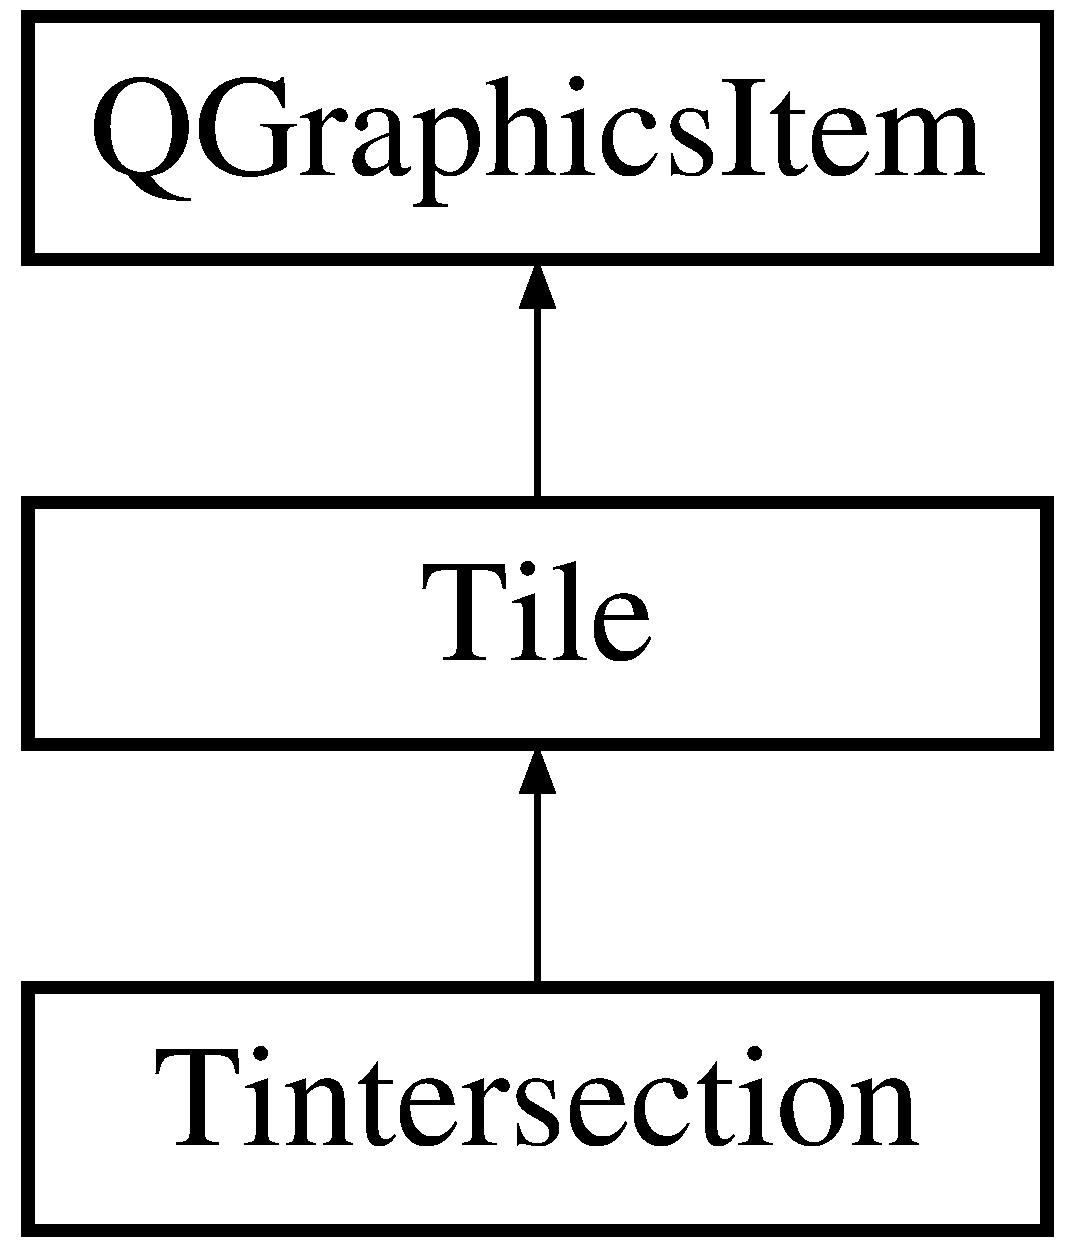
\includegraphics[height=3.000000cm]{class_tintersection}
\end{center}
\end{figure}
\subsection*{Public Member Functions}
\begin{DoxyCompactItemize}
\item 
\mbox{\hyperlink{class_tintersection_a6824eaa4942a78f9e0d5c3306ea870fa}{Tintersection}} (double nx, double ny, double nascent, int ndirection)
\item 
Q\+RectF \mbox{\hyperlink{class_tintersection_a5de6b3193359f459a05430612a409b65}{bounding\+Rect}} () const
\item 
Q\+String \mbox{\hyperlink{class_tintersection_a363e657adcc349bd47ea4517feaec8df}{get\+Type}} ()
\item 
void \mbox{\hyperlink{class_tintersection_a848fe29e044ad8a42d37be377b81f08c}{paint}} (Q\+Painter $\ast$painter, const Q\+Style\+Option\+Graphics\+Item $\ast$option, Q\+Widget $\ast$widget)
\item 
void \mbox{\hyperlink{class_tintersection_abac11aa16f7515f1ca0ef32389255d15}{rotate}} ()
\end{DoxyCompactItemize}
\subsection*{Additional Inherited Members}


\subsection{Constructor \& Destructor Documentation}
\mbox{\Hypertarget{class_tintersection_a6824eaa4942a78f9e0d5c3306ea870fa}\label{class_tintersection_a6824eaa4942a78f9e0d5c3306ea870fa}} 
\index{Tintersection@{Tintersection}!Tintersection@{Tintersection}}
\index{Tintersection@{Tintersection}!Tintersection@{Tintersection}}
\subsubsection{\texorpdfstring{Tintersection()}{Tintersection()}}
{\footnotesize\ttfamily Tintersection\+::\+Tintersection (\begin{DoxyParamCaption}\item[{double}]{nx,  }\item[{double}]{ny,  }\item[{double}]{nascent,  }\item[{int}]{ndirection }\end{DoxyParamCaption})}

Erstellt eine T-\/\+Kreuzung und fügt sie dem \mbox{\hyperlink{class_editor}{Editor}} hinzu. 
\begin{DoxyParams}{Parameters}
{\em x} & x-\/\+Koordinate der T-\/\+Kreuzung \\
\hline
{\em y} & y-\/\+Koordinate der T-\/\+Kreuzung \\
\hline
{\em ascent} & Steigung der T-\/\+Kreuzung \\
\hline
\end{DoxyParams}


\subsection{Member Function Documentation}
\mbox{\Hypertarget{class_tintersection_a5de6b3193359f459a05430612a409b65}\label{class_tintersection_a5de6b3193359f459a05430612a409b65}} 
\index{Tintersection@{Tintersection}!bounding\+Rect@{bounding\+Rect}}
\index{bounding\+Rect@{bounding\+Rect}!Tintersection@{Tintersection}}
\subsubsection{\texorpdfstring{bounding\+Rect()}{boundingRect()}}
{\footnotesize\ttfamily Q\+RectF Tintersection\+::bounding\+Rect (\begin{DoxyParamCaption}{ }\end{DoxyParamCaption}) const}

Erstellt ein Begrenzungsrechteck für das \mbox{\hyperlink{class_tile}{Tile}},Dieses wird sowohl zum zeichnen, als auch für weitere Interaktion benötigt \mbox{\Hypertarget{class_tintersection_a363e657adcc349bd47ea4517feaec8df}\label{class_tintersection_a363e657adcc349bd47ea4517feaec8df}} 
\index{Tintersection@{Tintersection}!get\+Type@{get\+Type}}
\index{get\+Type@{get\+Type}!Tintersection@{Tintersection}}
\subsubsection{\texorpdfstring{get\+Type()}{getType()}}
{\footnotesize\ttfamily Q\+String Tintersection\+::get\+Type (\begin{DoxyParamCaption}{ }\end{DoxyParamCaption})\hspace{0.3cm}{\ttfamily [virtual]}}

Gibt den Typen des \mbox{\hyperlink{class_tile}{Tile}} zurück \begin{DoxyReturn}{Returns}
Typ des \mbox{\hyperlink{class_tile}{Tile}} 
\end{DoxyReturn}


Reimplemented from \mbox{\hyperlink{class_tile_ad1dbea94d96060491a2dc4c7b92b31ab}{Tile}}.

\mbox{\Hypertarget{class_tintersection_a848fe29e044ad8a42d37be377b81f08c}\label{class_tintersection_a848fe29e044ad8a42d37be377b81f08c}} 
\index{Tintersection@{Tintersection}!paint@{paint}}
\index{paint@{paint}!Tintersection@{Tintersection}}
\subsubsection{\texorpdfstring{paint()}{paint()}}
{\footnotesize\ttfamily void Tintersection\+::paint (\begin{DoxyParamCaption}\item[{Q\+Painter $\ast$}]{painter,  }\item[{const Q\+Style\+Option\+Graphics\+Item $\ast$}]{option,  }\item[{Q\+Widget $\ast$}]{widget }\end{DoxyParamCaption})\hspace{0.3cm}{\ttfamily [virtual]}}

Zeichnet das \mbox{\hyperlink{class_tile}{Tile}} 
\begin{DoxyParams}{Parameters}
{\em painter} & Painter der zum Zeichnen benutzt wird \\
\hline
{\em option} & Optionen für das Zeichnen \\
\hline
{\em widget} & Widget in welches gezeichnet wird \\
\hline
\end{DoxyParams}


Reimplemented from \mbox{\hyperlink{class_tile_ab0a7262b6fab842a7a467fcb2f7592eb}{Tile}}.

\mbox{\Hypertarget{class_tintersection_abac11aa16f7515f1ca0ef32389255d15}\label{class_tintersection_abac11aa16f7515f1ca0ef32389255d15}} 
\index{Tintersection@{Tintersection}!rotate@{rotate}}
\index{rotate@{rotate}!Tintersection@{Tintersection}}
\subsubsection{\texorpdfstring{rotate()}{rotate()}}
{\footnotesize\ttfamily void Tintersection\+::rotate (\begin{DoxyParamCaption}{ }\end{DoxyParamCaption})\hspace{0.3cm}{\ttfamily [virtual]}}

Rotiert das \mbox{\hyperlink{class_tile}{Tile}} 

Reimplemented from \mbox{\hyperlink{class_tile_a15c3d8260c8950d3461e3ba2849cd141}{Tile}}.



The documentation for this class was generated from the following files\+:\begin{DoxyCompactItemize}
\item 
D\+:/swt1718-\/editor/bin/source/tintersection.\+h\item 
D\+:/swt1718-\/editor/bin/source/tintersection.\+cpp\end{DoxyCompactItemize}

\hypertarget{classturn}{}\section{turn Class Reference}
\label{classturn}\index{turn@{turn}}
Inheritance diagram for turn\+:\begin{figure}[H]
\begin{center}
\leavevmode
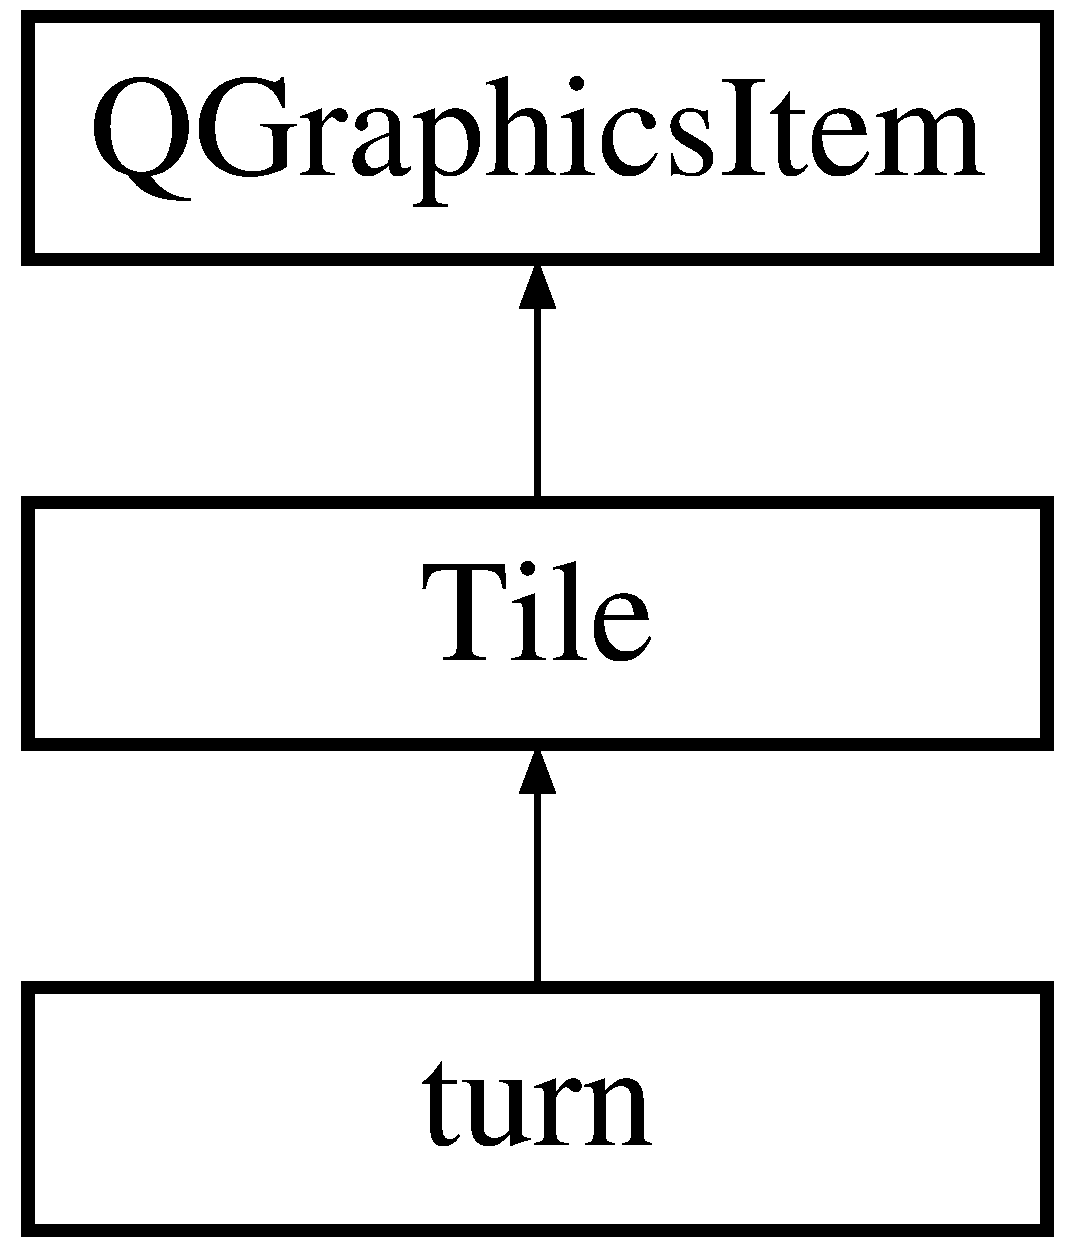
\includegraphics[height=3.000000cm]{classturn}
\end{center}
\end{figure}
\subsection*{Public Member Functions}
\begin{DoxyCompactItemize}
\item 
\mbox{\hyperlink{classturn_aa00a91ae978f5c08e8d8294ed438e785}{turn}} (double nx, double ny, double nascent, int ndirection)
\item 
Q\+RectF \mbox{\hyperlink{classturn_ad04b4ca6ec629c381d38bafbbf0c7052}{bounding\+Rect}} () const
\item 
Q\+String \mbox{\hyperlink{classturn_aee2e0c3c195f855186f12868232b18dd}{get\+Type}} ()
\item 
void \mbox{\hyperlink{classturn_a227bb1866470de67a42cc79890b5bf65}{paint}} (Q\+Painter $\ast$painter, const Q\+Style\+Option\+Graphics\+Item $\ast$option, Q\+Widget $\ast$widget)
\item 
void \mbox{\hyperlink{classturn_a91ab1e69c9ec2d7ded346a2701e1be1d}{rotate}} ()
\end{DoxyCompactItemize}
\subsection*{Additional Inherited Members}


\subsection{Constructor \& Destructor Documentation}
\mbox{\Hypertarget{classturn_aa00a91ae978f5c08e8d8294ed438e785}\label{classturn_aa00a91ae978f5c08e8d8294ed438e785}} 
\index{turn@{turn}!turn@{turn}}
\index{turn@{turn}!turn@{turn}}
\subsubsection{\texorpdfstring{turn()}{turn()}}
{\footnotesize\ttfamily turn\+::turn (\begin{DoxyParamCaption}\item[{double}]{nx,  }\item[{double}]{ny,  }\item[{double}]{nascent,  }\item[{int}]{ndirection }\end{DoxyParamCaption})}

Erstellt eine Kurve 
\begin{DoxyParams}{Parameters}
{\em x} & x-\/\+Position der Kurve \\
\hline
{\em y} & y-\/\+Position der Kurve \\
\hline
{\em ascent} & Steigung der Kurve \\
\hline
\end{DoxyParams}


\subsection{Member Function Documentation}
\mbox{\Hypertarget{classturn_ad04b4ca6ec629c381d38bafbbf0c7052}\label{classturn_ad04b4ca6ec629c381d38bafbbf0c7052}} 
\index{turn@{turn}!bounding\+Rect@{bounding\+Rect}}
\index{bounding\+Rect@{bounding\+Rect}!turn@{turn}}
\subsubsection{\texorpdfstring{bounding\+Rect()}{boundingRect()}}
{\footnotesize\ttfamily Q\+RectF turn\+::bounding\+Rect (\begin{DoxyParamCaption}{ }\end{DoxyParamCaption}) const}

Erstellt ein Begrenzungsrechteck für das \mbox{\hyperlink{class_tile}{Tile}},Dieses wird sowohl zum zeichnen, als auch für weitere Interaktion benötigt \mbox{\Hypertarget{classturn_aee2e0c3c195f855186f12868232b18dd}\label{classturn_aee2e0c3c195f855186f12868232b18dd}} 
\index{turn@{turn}!get\+Type@{get\+Type}}
\index{get\+Type@{get\+Type}!turn@{turn}}
\subsubsection{\texorpdfstring{get\+Type()}{getType()}}
{\footnotesize\ttfamily Q\+String turn\+::get\+Type (\begin{DoxyParamCaption}{ }\end{DoxyParamCaption})\hspace{0.3cm}{\ttfamily [virtual]}}

Gibt den Typen des \mbox{\hyperlink{class_tile}{Tile}} zurück \begin{DoxyReturn}{Returns}
Typ des \mbox{\hyperlink{class_tile}{Tile}} 
\end{DoxyReturn}


Reimplemented from \mbox{\hyperlink{class_tile_ad1dbea94d96060491a2dc4c7b92b31ab}{Tile}}.

\mbox{\Hypertarget{classturn_a227bb1866470de67a42cc79890b5bf65}\label{classturn_a227bb1866470de67a42cc79890b5bf65}} 
\index{turn@{turn}!paint@{paint}}
\index{paint@{paint}!turn@{turn}}
\subsubsection{\texorpdfstring{paint()}{paint()}}
{\footnotesize\ttfamily void turn\+::paint (\begin{DoxyParamCaption}\item[{Q\+Painter $\ast$}]{painter,  }\item[{const Q\+Style\+Option\+Graphics\+Item $\ast$}]{option,  }\item[{Q\+Widget $\ast$}]{widget }\end{DoxyParamCaption})\hspace{0.3cm}{\ttfamily [virtual]}}

Zeichnet das \mbox{\hyperlink{class_tile}{Tile}} 
\begin{DoxyParams}{Parameters}
{\em painter} & Painter der zum Zeichnen benutzt wird \\
\hline
{\em option} & Optionen für das Zeichnen \\
\hline
{\em widget} & Widget in welches gezeichnet wird \\
\hline
\end{DoxyParams}


Reimplemented from \mbox{\hyperlink{class_tile_ab0a7262b6fab842a7a467fcb2f7592eb}{Tile}}.

\mbox{\Hypertarget{classturn_a91ab1e69c9ec2d7ded346a2701e1be1d}\label{classturn_a91ab1e69c9ec2d7ded346a2701e1be1d}} 
\index{turn@{turn}!rotate@{rotate}}
\index{rotate@{rotate}!turn@{turn}}
\subsubsection{\texorpdfstring{rotate()}{rotate()}}
{\footnotesize\ttfamily void turn\+::rotate (\begin{DoxyParamCaption}{ }\end{DoxyParamCaption})\hspace{0.3cm}{\ttfamily [virtual]}}

Rotiert das \mbox{\hyperlink{class_tile}{Tile}} um 90 Grad 

Reimplemented from \mbox{\hyperlink{class_tile_a15c3d8260c8950d3461e3ba2849cd141}{Tile}}.



The documentation for this class was generated from the following files\+:\begin{DoxyCompactItemize}
\item 
D\+:/swt1718-\/editor/bin/source/turn.\+h\item 
D\+:/swt1718-\/editor/bin/source/turn.\+cpp\end{DoxyCompactItemize}

%--- End generated contents ---

% Index
\backmatter
\newpage
\phantomsection
\clearemptydoublepage
\addcontentsline{toc}{chapter}{Index}
\printindex

\end{document}
